% This template is borrowed from the Reed College LaTeX thesis template. Most of the work
% for the document class was done by Sam Noble (SN), as well as this
% template. Later comments etc. by Ben Salzberg (BTS). Additional
% restructuring and APA support by Jess Youngberg (JY).
% Your comments and suggestions are more than welcome; please email
% them to cus@reed.edu
%
% See http://web.reed.edu/cis/help/latex.html for help. There are a
% great bunch of help pages there, with notes on
% getting started, bibtex, etc. Go there and read it if you're not
% already familiar with LaTeX.
%
% Any line that starts with a percent symbol is a comment.
% They won't show up in the document, and are useful for notes
% to yourself and explaining commands.
% Commenting also removes a line from the document;
% very handy for troubleshooting problems. -BTS

% As far as I know, this follows the requirements laid out in
% the 2002-2003 Senior Handbook. Ask a librarian to check the
% document before binding. -SN

%%
%% Preamble
%%
% \documentclass{<something>} must begin each LaTeX document
\documentclass[12pt,twoside]{deuthesis}
% Packages are extensions to the basic LaTeX functions. Whatever you
% want to typeset, there is probably a package out there for it.
% Chemistry (chemtex), screenplays, you name it.
% Check out CTAN to see: http://www.ctan.org/
%%
\usepackage{graphicx,latexsym}
\usepackage{amsmath}
\usepackage{amssymb,amsthm}
\usepackage{longtable,booktabs,setspace}
\usepackage{chemarr} %% Useful for one reaction arrow, useless if you're not a chem major
\usepackage[hyphens]{url}
% Added by CII
\usepackage{hyperref}
\usepackage{lmodern}
\usepackage{float}
\floatplacement{figure}{H}
% End of CII addition
\usepackage{rotating}

% Next line commented out by CII
%%% \usepackage{natbib}
% Comment out the natbib line above and uncomment the following two lines to use the new
% biblatex-chicago style, for Chicago A. Also make some changes at the end where the
% bibliography is included.
%\usepackage{biblatex-chicago}
%\bibliography{thesis}


% Added by CII (Thanks, Hadley!)
% Use ref for internal links
\renewcommand{\hyperref}[2][???]{\autoref{#1}}
\def\chapterautorefname{Chapter}
\def\sectionautorefname{Section}
\def\subsectionautorefname{Subsection}
% End of CII addition

% Added by CII
\usepackage{caption}
\captionsetup{width=5in}
% End of CII addition

% \usepackage{times} % other fonts are available like times, bookman, charter, palatino

% Syntax highlighting #22
  \usepackage{color}
  \usepackage{fancyvrb}
  \newcommand{\VerbBar}{|}
  \newcommand{\VERB}{\Verb[commandchars=\\\{\}]}
  \DefineVerbatimEnvironment{Highlighting}{Verbatim}{commandchars=\\\{\}}
  % Add ',fontsize=\small' for more characters per line
  \usepackage{framed}
  \definecolor{shadecolor}{RGB}{248,248,248}
  \newenvironment{Shaded}{\begin{snugshade}}{\end{snugshade}}
  \newcommand{\AlertTok}[1]{\textcolor[rgb]{0.94,0.16,0.16}{#1}}
  \newcommand{\AnnotationTok}[1]{\textcolor[rgb]{0.56,0.35,0.01}{\textbf{\textit{#1}}}}
  \newcommand{\AttributeTok}[1]{\textcolor[rgb]{0.77,0.63,0.00}{#1}}
  \newcommand{\BaseNTok}[1]{\textcolor[rgb]{0.00,0.00,0.81}{#1}}
  \newcommand{\BuiltInTok}[1]{#1}
  \newcommand{\CharTok}[1]{\textcolor[rgb]{0.31,0.60,0.02}{#1}}
  \newcommand{\CommentTok}[1]{\textcolor[rgb]{0.56,0.35,0.01}{\textit{#1}}}
  \newcommand{\CommentVarTok}[1]{\textcolor[rgb]{0.56,0.35,0.01}{\textbf{\textit{#1}}}}
  \newcommand{\ConstantTok}[1]{\textcolor[rgb]{0.00,0.00,0.00}{#1}}
  \newcommand{\ControlFlowTok}[1]{\textcolor[rgb]{0.13,0.29,0.53}{\textbf{#1}}}
  \newcommand{\DataTypeTok}[1]{\textcolor[rgb]{0.13,0.29,0.53}{#1}}
  \newcommand{\DecValTok}[1]{\textcolor[rgb]{0.00,0.00,0.81}{#1}}
  \newcommand{\DocumentationTok}[1]{\textcolor[rgb]{0.56,0.35,0.01}{\textbf{\textit{#1}}}}
  \newcommand{\ErrorTok}[1]{\textcolor[rgb]{0.64,0.00,0.00}{\textbf{#1}}}
  \newcommand{\ExtensionTok}[1]{#1}
  \newcommand{\FloatTok}[1]{\textcolor[rgb]{0.00,0.00,0.81}{#1}}
  \newcommand{\FunctionTok}[1]{\textcolor[rgb]{0.00,0.00,0.00}{#1}}
  \newcommand{\ImportTok}[1]{#1}
  \newcommand{\InformationTok}[1]{\textcolor[rgb]{0.56,0.35,0.01}{\textbf{\textit{#1}}}}
  \newcommand{\KeywordTok}[1]{\textcolor[rgb]{0.13,0.29,0.53}{\textbf{#1}}}
  \newcommand{\NormalTok}[1]{#1}
  \newcommand{\OperatorTok}[1]{\textcolor[rgb]{0.81,0.36,0.00}{\textbf{#1}}}
  \newcommand{\OtherTok}[1]{\textcolor[rgb]{0.56,0.35,0.01}{#1}}
  \newcommand{\PreprocessorTok}[1]{\textcolor[rgb]{0.56,0.35,0.01}{\textit{#1}}}
  \newcommand{\RegionMarkerTok}[1]{#1}
  \newcommand{\SpecialCharTok}[1]{\textcolor[rgb]{0.00,0.00,0.00}{#1}}
  \newcommand{\SpecialStringTok}[1]{\textcolor[rgb]{0.31,0.60,0.02}{#1}}
  \newcommand{\StringTok}[1]{\textcolor[rgb]{0.31,0.60,0.02}{#1}}
  \newcommand{\VariableTok}[1]{\textcolor[rgb]{0.00,0.00,0.00}{#1}}
  \newcommand{\VerbatimStringTok}[1]{\textcolor[rgb]{0.31,0.60,0.02}{#1}}
  \newcommand{\WarningTok}[1]{\textcolor[rgb]{0.56,0.35,0.01}{\textbf{\textit{#1}}}}

% To pass between YAML and LaTeX the dollar signs are added by CII
\title{MAKİNE ÖĞRENMESİ YAKLAŞIMLARININ KARPAL TÜNEL SENDROMU CİDDİYET SINIFLAMASINDA KULLANILMASI}
%\author{Alper ENGİNAtadeniz SAYARCem GÖRENER} %Tek yazar için
\author{Alper ENGİN \\ Atadeniz SAYAR \\ Cem GÖRENER} %Çok yazar için
% The month and year that you submit your FINAL draft TO THE LIBRARY (May or December)
\date{Mayıs 2022}
\division{İSTATİSTİK BÖLÜMÜ}
\advisor{Dr.~Engin YILDIZTEPE}
\institution{FEN FAKÜLTESİ}
\degree{Bitirme Projesi Raporu}
%If you have two advisors for some reason, you can use the following
% Uncommented out by CII
% End of CII addition

%%% Remember to use the correct department!
\department{İstatistik Bölümü}
% if you're writing a thesis in an interdisciplinary major,
% uncomment the line below and change the text as appropriate.
% check the Senior Handbook if unsure.
%\thedivisionof{The Established Interdisciplinary Committee for}
% if you want the approval page to say "Approved for the Committee",
% uncomment the next line
%\approvedforthe{Committee}

% Added by CII
%%% Copied from knitr
%% maxwidth is the original width if it's less than linewidth
%% otherwise use linewidth (to make sure the graphics do not exceed the margin)
\makeatletter
\def\maxwidth{ %
  \ifdim\Gin@nat@width>\linewidth
    \linewidth
  \else
    \Gin@nat@width
  \fi
}
\makeatother

\renewcommand{\contentsname}{Table of Contents}
% End of CII addition

\setlength{\parskip}{0pt}

% Added by CII

\providecommand{\tightlist}{%
  \setlength{\itemsep}{0pt}\setlength{\parskip}{0pt}}

\Acknowledgements{
Tüm çalışma süresince yönlendiriciliği, katkıları ve yardımları ile yanımızda olan danışmanımız Dr.~Engin YILDIZTEPE 'ye ve böyle bir çalışmayı yapmamız için bize fırsat tanıyan Dokuz Eylül Üniversitesi Fen Fakültesi İstatistik Bölümüne teşekkür ederiz.\\
\strut \\
\strut \\
Alper ENGİN\\
Atadeniz SAYAR\\
Cem GÖRENER\\
}

\Dedication{

}

\Preface{
``MAKİNE ÖĞRENMESİ YAKLAŞIMLARININ KARPAL TÜNEL SENDROMU CİDDİYET SINIFLAMASINDA KULLANILMASI'' başlıklı bitirme projesi raporu tarafımdan okunmuş, kapsamı ve niteliği açısından bir Bitirme Projesi raporu olarak kabul edilmiştir.\\
\strut \\
\strut \\
Dr.~Engin YILDIZTEPE
}

\AbstractTR{
Özet, çalışmanın önemini ve faydasını anlatan bir bölüm degildir. Çalısmayı ana
hatlarıyla anlatacak ve 300 kelimeyi aşmayacak şekilde hazırlanmalıdır. En az üç en
çok beş anahtar kelime ilgili yere yazılmalıdır.

\par

ikinci paragraf buradan başlar\\
\strut \\
\textbf{Anahtar Kelimeler:} anahtar kelime 1, anahtar kelime 2, anahtar kelime 3
}

\Abstract{
The preface pretty much says it all.

\par

Second paragraph of abstract starts here.\\
\strut \\
\textbf{Keywords:} keyword1, keyword2, keyword3
}


	\AtBeginDocument{\renewcommand{\chaptername}{Bölüm}}
 \AtBeginDocument{\renewcommand{\contentsname}{İçerik}}
 \AtBeginDocument{\renewcommand{\listfigurename}{Şekil Listesi}}
 \AtBeginDocument{\renewcommand{\listtablename}{Tablo Listesi}}
 \AtBeginDocument{\renewcommand{\figurename}{Şekil}}
 \AtBeginDocument{\renewcommand{\tablename}{Tablo}}
 \AtBeginDocument{\renewcommand{\appendixname}{Ek}}
% End of CII addition
%%
%% End Preamble
%%
%
\begin{document}

% Everything below added by CII
  \maketitle

\frontmatter % this stuff will be roman-numbered
\pagestyle{empty} % this removes page numbers from the frontmatter
\begin{preface}
	``MAKİNE ÖĞRENMESİ YAKLAŞIMLARININ KARPAL TÜNEL SENDROMU CİDDİYET SINIFLAMASINDA KULLANILMASI'' başlıklı bitirme projesi raporu tarafımdan okunmuş, kapsamı ve niteliği açısından bir Bitirme Projesi raporu olarak kabul edilmiştir.\\
 \strut \\
 \strut \\
 Dr.~Engin YILDIZTEPE
\end{preface}
  \begin{acknowledgements}
    Tüm çalışma süresince yönlendiriciliği, katkıları ve yardımları ile yanımızda olan danışmanımız Dr.~Engin YILDIZTEPE 'ye ve böyle bir çalışmayı yapmamız için bize fırsat tanıyan Dokuz Eylül Üniversitesi Fen Fakültesi İstatistik Bölümüne teşekkür ederiz.\\
    \strut \\
    \strut \\
    Alper ENGİN\\
    Atadeniz SAYAR\\
    Cem GÖRENER\\
  \end{acknowledgements}
\begin{abstractTR}
	Özet, çalışmanın önemini ve faydasını anlatan bir bölüm degildir. Çalısmayı ana
 hatlarıyla anlatacak ve 300 kelimeyi aşmayacak şekilde hazırlanmalıdır. En az üç en
 çok beş anahtar kelime ilgili yere yazılmalıdır.

 \par

 ikinci paragraf buradan başlar\\
 \strut \\
 \textbf{Anahtar Kelimeler:} anahtar kelime 1, anahtar kelime 2, anahtar kelime 3
\end{abstractTR}
\begin{abstract}
	The preface pretty much says it all.

 \par

 Second paragraph of abstract starts here.\\
 \strut \\
 \textbf{Keywords:} keyword1, keyword2, keyword3
\end{abstract}

  \hypersetup{linkcolor=black}
  \setcounter{tocdepth}{2}
  \tableofcontents

  \listoftables

  \listoffigures


% This was added by EY
\newlength{\cslhangindent}
\setlength{\cslhangindent}{1.5em}
\newenvironment{CSLReferences}%
  {}%
  {\par}
\newenvironment{cslreferences}%
  {}%
  {\par}

\mainmatter % here the regular arabic numbering starts
\pagestyle{fancyplain} % turns page numbering back on


\hypertarget{KTSTanim}{%
\chapter{Karpal Tünel Sendromu}\label{KTSTanim}}

Karpal tünel sendromu, medyan sinirin karpal tüneli içerisinde baskıya uğraması sonucu ortaya çıkan semptomların genel adıdır (Werner ve Andary, 2002).\\
Tarihte ilk kez Pajet tarafından, 1854 yılında medyan sinir hasarının bulguları gözlenirken tanımlanmıştır (Pfeffer, Gelberman, Boyes ve Rydevik, 1988).\\
Karpal tünel sendromu (KTS), tanımlanması ve terimleştirilmesi ilk olarak 1947 yılında Brain, Wright ve Wilkinson tarafından yapılmıştır (Love, 1955).
\begin{figure}

{\centering 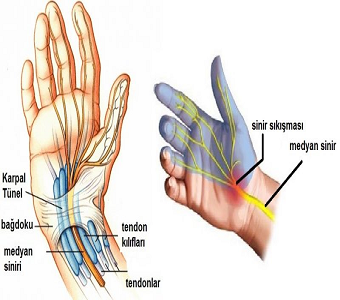
\includegraphics[width=4.72in]{figure/karpal_tunnel} 

}

\caption{Karpal Tünel Anatomisi ve Medyan Sinirin Sıkışması}\label{fig:unnamed-chunk-1}
\end{figure}
\hypertarget{KTSEpidemiyoloji}{%
\section{Epidemiyoloji}\label{KTSEpidemiyoloji}}

KTS prevalansı kadınlarda \%3 ila \%3.4 arasında, erkeklerde ise \%0.6 ila \% 2.7 arasında olarak
belirlenmiştir. İnsidans ise kadınlarda 100.000'de 140, erkeklerde 100.000'de 52 olarak saptanmıştır.
Kadınlarda genellikle menopoz dönemimde sıklıkla görülmüş olsa da hem erkek hem de kadınlarda
gözlenme sıklığı yaş ile doğru orantılıdır. Özellikle 20 ila 50 yaş arasında daha sıktır. KTS'nin \%40 ila \%60 oranında her iki elde de başlayabileceği çeşitli yayınlarda bildirilmiş olup, iki elde de görüldüğü olgularda baskın elin genellikle semptomları daha önce ve daha şiddetli gösterdiği söylenebilir. KTS tek elde görüldüğü durumlarda ise genellikle semptomlar baskın elde görülür (Bagatur, 2006).

\hypertarget{KTSEtiyoloji}{%
\section{Etiyoloji}\label{KTSEtiyoloji}}

Karpal tünel sendromunun en sık nedeni; herhangi bir etiyolojik etkenin saptanamadığı idiopatik KTS'dir. İdiopatik KTS'de ailesel yatkınlık, obezite, VKİ fazla olması, kara şeklinde bilek yapısı gibi
kişisel faktörlerin etken olduğu düşünülmektedir. Günlük yaşamda ki mekanik etkenler de idiopatik KTS
üzerinde etkin rol oynamaktadır. Montaj işinde çalışan işçiler, fabrika çalışanları, klavye ve bilgisayar
kullananlarda olduğu gibi el bilek fleksiyonun aktif olarak yapıldığı belli hareketlerin çok sık
tekrarlanması da KTS ile ilişkili bulunmuştur (Robbins, 1963).

\hypertarget{KTSSemptom}{%
\section{Semptomlar}\label{KTSSemptom}}

Hastalığın şiddetine bağlı olarak semptomlar değişkendir. Erken evrelerde medyan sinirin duyusal
liflerinin tutulumuna bağlı şikayetler görülür. En yaygın semptom el bileğinin merkezinden uzak
dokularda sızlama ve uyuşuklukla beraber yanıcı tarzda ağrıdır. Başparmak tarafından itibaren ilk üç
parmak ve dördüncü parmağın yanal yarısı etkilenir. Daha ileri dönemlerde el ayasında kas
güçsüzlüğü ve körelme meydana gelir . Bu hastalarda elde, özellikle aktivite ile artan beceriksizlik ve objeleri kavramada kuvvetsizlik görülür (Aroori ve Spence, 2008).

\hypertarget{KTSTani_Ciddi}{%
\section{Tanı ve Ciddiyet Değerlendirmesi}\label{KTSTani_Ciddi}}

Karpal tünel sendromunda tanı koymak için hastanın hikayesi, klinik semptomlar, fizik muayene bulguları ve bu bulguları destekleyen çeşitli testler kullanılmaktadır(Ghasemi-Rad ve diğerleri, 2014).
Bu testler elektronörofizyolojik, provokatif testler ve tıbbi görüntülemeye dayanan testlerdir.
Elektronörofizyolojik testler karpal Tünel'e bağlanan elektrotlar ile elektrik sinyallerinin incelenmesi ve sonuçların bilgisayar ile yorumlanmasına dayananan testlerdir.

\begin{figure}

{\centering 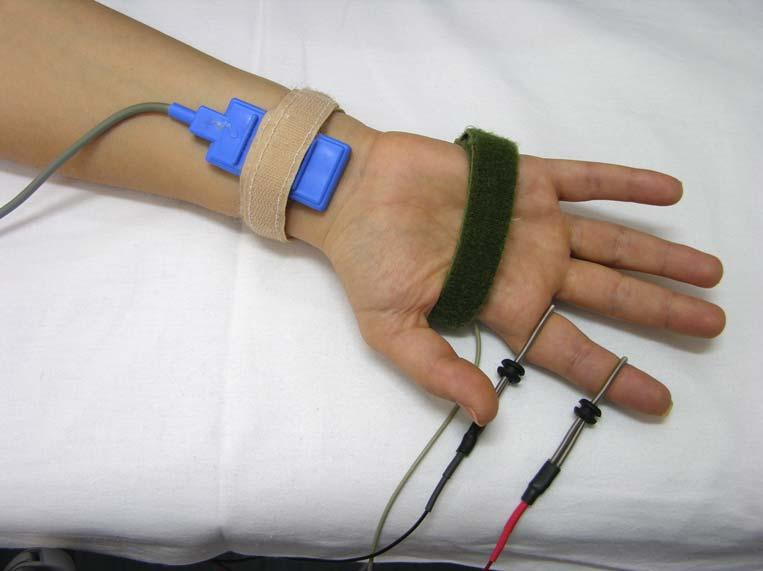
\includegraphics[width=0.49\linewidth,height=0.18\textheight]{figure/noropati_test} 

}

\caption{Elektronörofizyolojik Test (Kumaş, 2005)}\label{fig:unnamed-chunk-2}
\end{figure}
Provokatif testler hastanın bilek ve parmak eklemlerine fiziksel baskı uygulayacak şekilde bir takım
testler uygulanması ve alınan sonuçların değerlendirmesine dayanan deneysel test yöntemleridir.
Tanısal testler genellikle karpal tüneli görüntülemeye dayanan testlerdir.
\begin{itemize}
\item
  Phalen Testi
  \begin{itemize}
  \tightlist
  \item
    60 saniye boyunca parmaklar ayak ucuna bakacak şekilde el dış yüzleri birleştirilir. Meydan sinir bölgesinde karıncalanma oluşur veya artarsa test pozitiftir.
  \end{itemize}
\item
  Ters Phalen testi
  \begin{itemize}
  \tightlist
  \item
    60 saniye boyunca parmaklar yukarı bakacak şekilde el dış yüzleri birleştirilir. Meydan sinir bölgesinde karıncalanma oluşur veya artarsa test pozitiftir.
  \end{itemize}
\item
  Tinel testi
  \begin{itemize}
  \tightlist
  \item
    Uygulayıcı tarafından karpal tünelin üstüne perküsyon yapılır. Medyan sinir bölgesinde karıncalanma ve elektrik şoku hissi oluşursa test pozitiftir (Kurt, 2020).
  \end{itemize}
\item
  Karpal kompresyon testi
  \begin{itemize}
  \tightlist
  \item
    El bileği düz tutulurken medyan sinirin yakınına başparmak ile bastırılır. Medyan sinir bölgesinde karıncalanma oluşur veya artarsa test pozitiftir.
  \end{itemize}
\item
  Gerilmiş median sinir stres (GMSS) testi
  \begin{itemize}
  \tightlist
  \item
    Medyan sinir hareketliliğinin azaldığı durumlarda medyan sinirin gerilerek lokal iskeminin arttırılması mantığına dayanır.
  \end{itemize}
\end{itemize}
\begin{figure}

{\centering 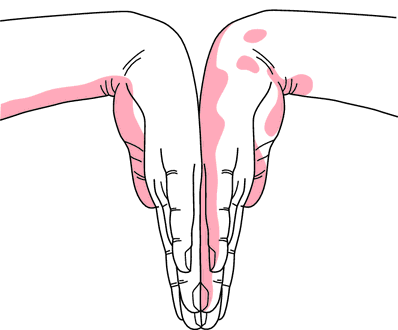
\includegraphics[width=0.49\linewidth,height=0.18\textheight]{figure/phalen} 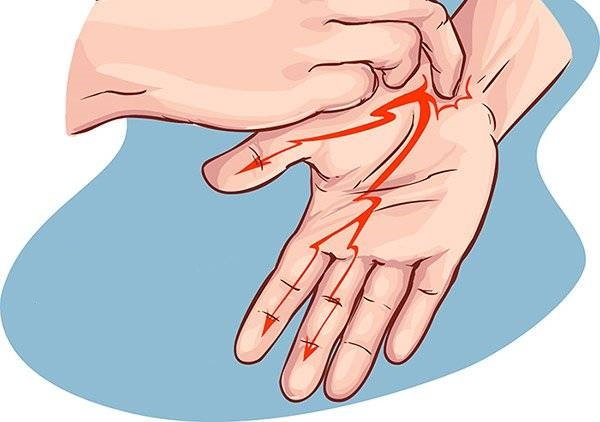
\includegraphics[width=0.49\linewidth,height=0.18\textheight]{figure/tinel} 

}

\caption{Phalen ve Tinel Testi}\label{fig:unnamed-chunk-3}
\end{figure}
\begin{figure}

{\centering 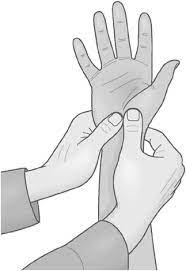
\includegraphics[width=0.49\linewidth,height=0.18\textheight]{figure/karpal_komp} 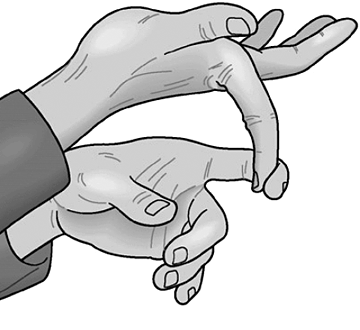
\includegraphics[width=0.49\linewidth,height=0.18\textheight]{figure/gerilmis} 

}

\caption{Karpal kompresyon ve GMSS Testi }\label{fig:unnamed-chunk-4}
\end{figure}
Görüntülemeye dayalı testlerde el bileği ve parmakların hareketi sırasında karpal tünel içerisindeki değişiklikleri ve medyan sinirin hareketlerini yorumlayarak hastaya tanı koymayı kolaylaştırır fakat hastalığın şiddeti hakkında bilgi vermez.
\begin{itemize}
\item
  Ultrasonografi
\item
  Düz radyografi
\item
  Bilgisayarlı tomografi
\item
  Manyetik rezonans görüntüleme
\end{itemize}
\begin{figure}

{\centering 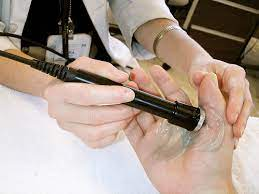
\includegraphics[width=0.49\linewidth,height=0.22\textheight]{figure/ultraradyo} 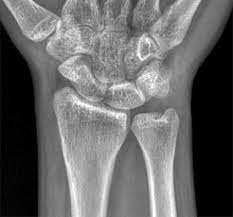
\includegraphics[width=0.49\linewidth,height=0.22\textheight]{figure/radyog} 

}

\caption{Ultrasonografi ve Düz radyografi }\label{fig:unnamed-chunk-5}
\end{figure}
\begin{figure}

{\centering 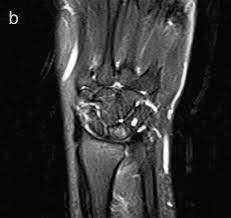
\includegraphics[width=0.49\linewidth,height=0.22\textheight]{figure/bt} 

}

\caption{Bilgisayarlı tomografi }\label{fig:unnamed-chunk-6}
\end{figure}
İdiopatik karpal tünel sendromunda hastalığın tanımlanmasında Boston Karpal Tünel Sendromu
Anketi(BKTSA) kullanılmaktadır (Levine ve diğerleri, 1993). Bu ankete farklı dillere çevrilmiş ve ülkelere göre uyarlanmıştır. Anketin amacı hastanın yanıtlarına göre bir ciddiyet sınıflandırması yapmaktır. Anketin Türkçe versiyonu Sezgin ve ark. (Sezgin ve diğerleri, 2006) tarafından yayımlanmıştır , ancak BKTSA sadece hastaların verdiği yanıtlara dayanarak bir semptom şiddeti belirlemeyi amaçlar.

Teknolojinin hızla gelişmesi ile birlikte hastalara uygulanan testlerin sonuçlarının toplanmasının kolaylaşmasının yanı sıra testlerin sonuçlarına bağlı olarak hastaya tanı koymak ve tanının şiddetini ve derecesini tespit etmek oldukça kolaylaşmıştır.\\
Makine öğrenmesi ve Yapay zeka uygulamalarının yaygınlaşması ile birlikte bu yöntemlerin tıp alanında da kullanımı artmıştır.

Makine öğrenmesi yöntemlerinin KTS tanısında kullanılmaına örnek olarak.
Ardakani ve ark. (Ardakani ve diğerleri, 2020) tarafından hasta olduğu bilinen kişilerden elde edilen bilgisayarlı tomografi görüntüleri, derin öğrenme metodları kullanılarak başka kişilerin hasta olup olmadığını tespit etmek için kullanılmıştır.\\
Bir diğer çalışma ise 2021 yılında Koyama ve ark. (Koyama ve diğerleri, 2021) tarafından geliştirilen bir mobil uygulama sayesinde hastaların ekranın farklı yerlerinde çıkan cisimlere ulaşma sürelerini baz alarak hastalığın evresini tahminlemeyi amaçlamıştır. Bu uygulama hastanın kendi kendine ev ortamında hastalığına ön tanı koyabilmesi açısından yararlı olabilir.\\
Bunların yanı sıra KTS ciddiyet skoru belirlemek için makine öğrenmesi yöntemlerini kullanan çalışmalar da yapılmaktadır.
Güncel bir çalışmada Park ve ark. (Park ve diğerleri, 2021) 1037 hastadan elde edilen verileri farklı makine öğrenmesi yöntemlerinde kullanarak KTS ciddiyet sınıflandırmasını tahmin etmeyi amaçlamışlardır.

\hypertarget{yontem}{%
\chapter{Yöntem}\label{yontem}}

Bu bölümde uygulama kısmında kullanılan sınıflama algoritmalarına değinilmiştir.

\hypertarget{knn}{%
\section{K - En Yakın Komşuluk Algoritamsı (K-NN)}\label{knn}}

K-NN algoritması, Cover ve Hart tarafından önerilen, örnek veri noktasının bulunduğu sınıfın ve en yakın komşunun, k değerine göre belirlendiği bir sınıflandırma yöntemidir (Cover ve Hart, 1967).\\
K-NN algoritması, en temel örnek tabanlı öğrenme algoritmaları arasındadır. Örnek tabanlı öğrenme algoritmalarında, öğrenme işlemi eğitim setinde tutulan verilere dayalı olarak gerçekleştirilmektedir. Yeni karşılaşılan bir örnek, eğitim setinde yer alan örnekler ile arasındaki benzerliğe göre sınıflandırılmaktadır (Mitchell ve Learning, 1997). K-NN algoritmasında, eğitim setinde yer alan örnekler n boyutlu sayısal nitelikler ile belirtilir. Her örnek n boyutlu uzayda bir noktayı temsil edecek biçimde tüm eğitim örnekleri n boyutlu bir örnek uzayında tutulur. Bilinmeyen bir örnek ile karşılaşıldığında, eğitim setinden ilgili örneğe en yakın k tane örnek belirlenerek yeni örneğin sınıf etiketi, k en yakın komşusunun sınıf etiketlerinin çoğunluk oylamasına göre atanır (Mining, 2006).

\hypertarget{k-nn-parametleri}{%
\subsection{K-NN Parametleri}\label{k-nn-parametleri}}

K-NN algoritmasında performansı etkileyen 3 adet hiper parametre mevcuttur. Bunlar; Uzaklık ölçütü, komşu sayısı(k) ve ağırlıklandırma yöntemidir.

\hypertarget{uzaklux131k-uxf6luxe7uxfctuxfc}{%
\subsubsection{Uzaklık Ölçütü}\label{uzaklux131k-uxf6luxe7uxfctuxfc}}

En bilinen ve yaygın olarak kullanılan 3 uzaklık;
\begin{itemize}
\tightlist
\item
  Minkowski Uzaklığı\\
\item
  Öklid Uzaklığı\\
\item
  Manhattan Uzaklığı
\end{itemize}
\hypertarget{komux15fu-sayux131sux131-k}{%
\subsubsection{Komşu Sayısı (k)}\label{komux15fu-sayux131sux131-k}}

En yakın komşuluk algoritmasında komşu sayısına (k) göre sınıflama yapıldığından algoritma için en önemli parametresi olduğu söylenebilir. k = 5 olarak belirlendiğinde yeni gözlem kendisine en yakın 5 değer baz alınarak sınıflandırılır.

\hypertarget{aux11fux131rlux131klandux131rma}{%
\subsubsection{Ağırlıklandırma}\label{aux11fux131rlux131klandux131rma}}

Komşular için ağırlık değerleri atanması ile sınıflandırılmakta olan örneğe daha yakın olan komşu örneklerin, çoğunluk oylamasına daha fazla katkı koyması amaçlanır. En çok kullanılan ağırlık değeri atama yöntemleri, her bir komşunun ağırlığının, d, komşular arası uzaklık olmak üzere, 1/d ya da \(1/d^2\) şeklinde alınmasıdır (Doad ve Bartere, 2013).

\hypertarget{random_forest}{%
\section{Rassal Ormanlar}\label{random_forest}}

Rassal ormanlar sınıflandırıcısı, her biri farklı girdi vektörlerinden oluşan ve her ağacın yalnızca bir sınıfa oy verdiği karar ağaçlarının kombinasyonudur (Leo Breiman, 1999). Rassal ormanlar sınıflandırması ağaç derinliğini büyütmek için her dalda rastgele değişkenleri içerir.

Karar ağaçlarını modellemek, bir budama metodu ve nitelik seçme ölçütü seçmeyi gerektirir. Karar ağacının tüme varımı için kullanınlan bir sürü nitelik seçme yaklaşımı vardır ve çoğu yaklaşımlar niteliğe direkt olarak kalite ölçümü belirler. Karar ağacının tümü varmında ki en sık kullanılan nitelik seçme ölçümleri Information gain ratio kriteri ve Gini indexidir (L. Breiman, Friedman, Olshen ve Stone, t.y.).

Verilen herhangi bir eğitim verisi için gini index o verinin hangi sınıfa ait olduğu olasılığını hesaplar.

\[\begin{aligned}
\sum \sum_{j \neq i}(f(C_{i}, T) /|T|)(f(C_{j}, T) /|T|)
\end{aligned}\]
Bu denklemde \(f(C_{i}, T) /|T|)\) seçilen gözlemin \(C_{i}\) sınıfa ait olma olasılığıdır.

Her seferinde bir ağaç, değişkenlerin bir kombinasyonunu kullanarak yeni eğitim verisi üzerinde en büyük derinliğe kadar büyür. Son derinliğine ulaşmış bu ağaçlar budanmamıştır. Bu durum, (Quinlan, 2014) veya diğer karar ağacı methodlarına göre rassal ormanlanların en büyük avantajıdır. Bazı durumlarda maliyet ve karmaşıklığı minimum yapabilmek için rassal ormanlar içerisindeki karar ağaçlarına budama yapılır. Budama parametresi olan `ccp\_alpha' değerinden daha küçük olan en büyük maliyet ve karmaşıklık değerini bulunana kadar karar ağacı budanır.

Sonuç olarak, rastgele ağaçlar methodu, kullanıcının herhangi bir değer belirleyebildiği, N kadar büyüyecek karar ağaçları içerir. Yeni veri setini sınıflandırmak için, seçilen maksimum değişken sayısına göre veri setinde ki rastgele olarak paylaştırılmış her gözlem, N kadar karar ağacının her biri tarafından sınıflandırılır. Bu durum için ormanlar en fazla oya sahip sınıfı seçer.\\

\begin{figure}

{\centering 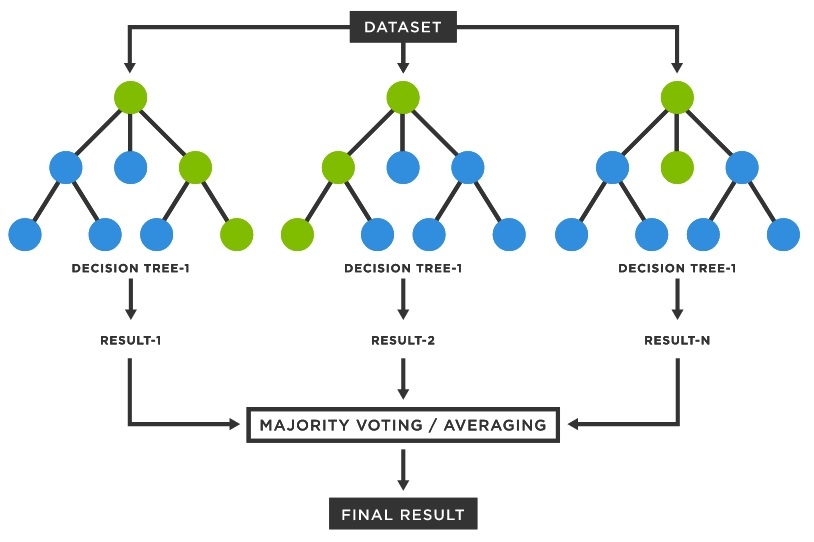
\includegraphics[width=1\linewidth,height=0.48\textheight]{figure/rf_example} 

}

\caption{Rassal Ormanlar Model Örneği (TIBCO, t.y.)}\label{fig:unnamed-chunk-7}
\end{figure}
\hypertarget{xgboost}{%
\section{XGBoost}\label{xgboost}}

Bu bölümde XGboost algoritmasına ve XGBoost algoritmasının daha iyi anlaşabilmesi için XGBoost'un altyapısını oluşturan gradyan arttırma algoritmasına değinilmiştir.

\hypertarget{gradyan-arttux131rux131mux131}{%
\subsection{Gradyan Arttırımı}\label{gradyan-arttux131rux131mux131}}

Gradyan artırma fikri, Leo Breiman'ın , artırmanın uygun bir maliyet fonksiyonu üzerinde bir optimizasyon algoritması olarak yorumlanabileceği gözleminden kaynaklanmıştır (Leo Breiman, 1997). Açık regresyon gradyan artırma algoritmaları daha sonra Jerome H. Friedman (Friedman, 2001), tarafından Llew Mason, Jonathan Baxter, Peter Bartlett ve Marcus Frean'ın daha genel fonksiyonel gradyan artırma perspektifiyle eş zamanlı olarak geliştirildi (Mason, Baxter, Bartlett ve Frean, 1999).

Gradyan artırma, genellikle karar ağaçları gibi zayıf tahmin modelleri topluluğu şeklinde bir tahmin modeli üreten, regresyon, sınıflandırma ve diğer görevler için bir makine öğrenimi tekniğidir. Bir karar ağacı zayıf öğrenen ise, ortaya çıkan algoritmaya genellikle rastgele ormandan daha iyi performans gösteren gradyan destekli ağaçlar denir (Hastie, Tibshirani ve Friedman, 2009). Modeli, diğer artırma yöntemlerinin yaptığı gibi aşamalı bir şekilde oluşturur ve keyfi bir türevlenebilir kayıp fonksiyonun optimizasyonuna izin vererek bunları genelleştirir.\\
Gradyan Arttırımı Algoritması ;
\begin{itemize}
\item
  Adım 1 : \(\{(x_i,y_i)\}_{i=1}^n\) şeklinde veri ve türevlenebilir bir kayıp fonksiyonu \(L(y_i,F(x))\) tanımlanır.
\item
  Adım 2 : \(F_0(x) = \min\limits_{\gamma}\,\sum_{i=1}^{n}L(y_i,\gamma)\) \(\gamma\) = Tahmin Değeri olacak şekilde başlangıç değeri (\(F_0(x)\)) minumum olacak şekilde türevlenip 0'a eşitlenir ve \(F_0(x)\)'in minumum değeri elde edilir.
\item
  Adım 3 :
  \begin{itemize}
  \item
    Adım 3.1 : m=1 \(\to\) M'e kadar bir önceki tahmin değerine göre hatalar hesaplanır. (M burada sınıflandırma veya regresyon ağacı sayısıdır)
    \[r_{im} = -\left[\frac{\partial L(y_i,F(x_i)}{\partial F(x_i)}\right]_{F(x)=F_{m-1}(x)}\:\,i=1 \to n\]
  \item
    Adım 3.2 : \(r_{im}\) değerlerine göre regresyon veya sınıflandırma ağacı eğitilir ve \(R_{jm}\) terminal bölgeleri oluşturulur.
  \item
    Adım 3.3 : Her bir yaprak için çıktı değeri hesaplanır.
    \[\gamma_{jm} = \min\limits_{\gamma}\,\sum_{x_i\in R_{ij}}L(y_i,F_{m-1}(x_i)+\gamma)\]
    Yine aynı şekilde kayıp fonksiyonunun türevi alınır ve değerler toplanıp sınıfa eşitlenir. Çıkan sayı yaprağın değeridir.
  \item
    Adım 3.4 : Her gözlem için tahmin oluşturulur.
    \[F_m(x) = F_{m-1}(x) + \nu\sum_{j=1}^{J_m}\gamma_{jm}I(x\in R_{jm})\]
    Formül incelendiğinde yeni ağacın tahmin değerinin önceki ağacın tahmin değeri + (öğrenme düzeyi \(\times\) yeni ağacın değeri) olduğu görülmektedir.
  \end{itemize}
\end{itemize}

\begin{figure}

{\centering 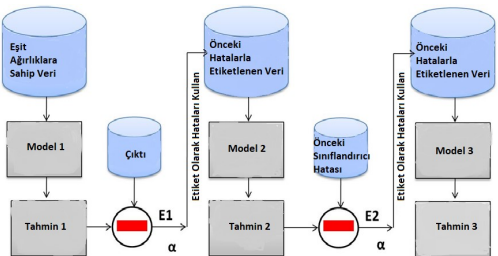
\includegraphics[width=1\linewidth,height=0.4\textheight]{figure/gb-dixit} 

}

\caption{Gradyan Arttırma Çalışma Mantığı (Dikker, 2017)}\label{fig:unnamed-chunk-8}
\end{figure}
\hypertarget{xgboost-aux15fux131rux131-gradyan-arttux131rux131mux131}{%
\subsection{XGBoost (Aşırı Gradyan Arttırımı)}\label{xgboost-aux15fux131rux131-gradyan-arttux131rux131mux131}}

XGBoost, temeli gradyan arttırımı ve karar ağacı algoritmalarına dayanan bir makine gözetimli öğrenme tekniğidir.
XGBoost algoritmasının orijinal hali Friedman tarafından 2002 yılında geliştirilmiştir (Dikker, 2017). Sonrasında Washington Üniversitesi'nde iki araştırmacı olan TianqiChen ve Carlos Guestrin tarafından SIGKDD (Bilgi İşlem Makinalarının Bilgi Keşfi ve Veri Madenciliği Özel İlgi Grubu Derneği) 2016 konferansında makale olarak sunulmuştur ve makine öğrenme dünyasında çok popüler olmuştur (Chen ve Guestrin, 2016).

XGBoost, yüksek tahmin etme gücüne sahip olup, diğer algoritmalardan 10 kat daha hızlıdır. Ayrıca XGBoost, genel performansı iyileştiren ve aşırı uyum ya da aşırı öğrenmeyi azaltan bir dizi düzetlme işlemleri içermektedir (Yangın, 2019).

Gradyan arttırımı, güçlü bir sınıflandırıcı oluşturmak için, bir dizi zayıf sınıflandırıcıyı arttırma ile birleştiren topluluk yöntemidir. Güçlü öğrenici, temel bir öğrenici ile başlayarak yinelemeli olarak eğitilmektedir. Hem gradyan arttırımı hem de XGBoost aynı prensibi izlemektedir. Aralarındaki temel farklar uygulama detaylarında yatmaktadır. XGBoost, farklı düzeltme teknikleri kullanarak, ağaçların karmaşıklığını kontrol ederek daha iyi bir performans elde etmeyi başarmaktadır (Salam Patrous, 2018).
\begin{itemize}
\item
  Adım 1 : \(\{(x_i,y_i)\}_{i=1}^n\) şeklinde veri ve türevlenebilir bir kayıp fonksiyonu \(L(y_i,F(x))\) tanımlanır. XGBoost algoritması kayıp fonksiyonu olarak \[L(y_i,P_i) = -[y_{i}log(P_i)+(1-y_i)log(1-P_i)]\] fonksiyonunu kullanır burada \(P_i\) tahmin değerine eşittir.
\item
  Adım 2 : \(F_0(x) = \min\limits_{\gamma}\,\sum_{i=1}^{n}L(y_i,\gamma)\), \(\gamma\) = Tahmin Değeri olacak şekilde başlangıç değeri (\(F_0(x)\)) minumum olacak şekilde türevlenip 0'a eşitlenir ve \(F_0(x)\)'in minumum değeri elde edilir.
\item
  Adım 3 : Her bir yaprak için optimal çıktı değerini elde etmek amacı ile aşağıdaki denklemden yararlanılır.
  \begin{equation}
    \label{eq1}
    L(y,P_i+0_{value}) \approx L(y,P_i) + gO_{value} + \frac{1}{2}hO_{value}^2
  \end{equation}
  \[
  L(y,P_i) = L(y_i,log(Odds)_i) = -y_{i}log(Odds) + log\left(1 + e^{log(Odds)}\right)
  \]
  \[
    g = \left[\frac{d}{dlog(Odds)}L(y_i,log(Odds)_i)\right] = -y_i + \frac{e^{log(Odds)_i}}{1 + e^{log(Odds)_i}} = -(y_i - P_i)
  \]
  \[
    h = \left[\frac{d^2}{dlog(Odds)^2}L(y_i,log(Odds)_i)\right] = \frac{e^{log(Odds)_i}}{(1 + e^{log(Odds)_i})^2} = P_i\times (1-P_i)
  \]
  \begin{itemize}
  \tightlist
  \item
    Adım 3.1 : Denlem \ref{eq1}'den yararlanıldığı takdirde aşağıdaki denklem elde edilmektedir.
    \begin{equation}
      (g_1 + g_2 + \ldots + g_n)O_{value} + \frac{1}{2}(h_1 + h_2 + \ldots + h_n + \lambda)O_{value}^2
      \label{eq2}
      \end{equation}
  \item
    Adım 3.2 : Çıktı değerini elde edebilmek için Denklem \ref{eq2}'de elde edilen denklemin \(O_{value}\)'ya göre türevi alınarak 0'a eşitlenir.
    \[
      \frac{d}{dO_{value}} (g_1 + g_2 + \ldots + g_n)O_{value} + \frac{1}{2}(h_1 + h_2 + \ldots + h_n + \lambda)O_{value}^2 = 0
      \]
    \begin{equation}
      O_{value} = \frac{-(g_1 + g_2 + \ldots + g_n)}{(h_1 + h_2 + \ldots + h_n + \lambda)}
      \label{eq3}
      \end{equation}
  \item
    Adım 3.3 : Elde edilen Denklem \ref{eq3} yardımı ile benzerlik skoru hesaplanabilir. Bu nokta Benzerlik skoru yardımı ile karar noktasına karar verilir. Benzerlik skoru ne kadar düşükse o karar noktasının veri setini daha keskin bir biçimde ayrıştırdığı düşünülür.
    \begin{equation}
      \label{eq4}
      \textrm{Benzerlik Skoru} = \frac{(g_1 + g_2 + \ldots + g_n)^2}{(h_1 + h_2 + \ldots + h_n + \lambda)}
      \end{equation}
  \end{itemize}
\item
  Adım 4 : Sırası ile Denklem \ref{eq4} ve \ref{eq3}, M adet ağaç için hesaplandıktan sonra her ağacın çıktı sonucu eta (öğrenme düzeyi) ile çarpılıp kümülatif olarak toplanır. Son olarak elde edilen ağaçların kümülatif toplamı başta hesaplanan ilk değer ile toplanıp gözlem için tahmin verisi oluşturulur.
\end{itemize}
\begin{figure}

{\centering 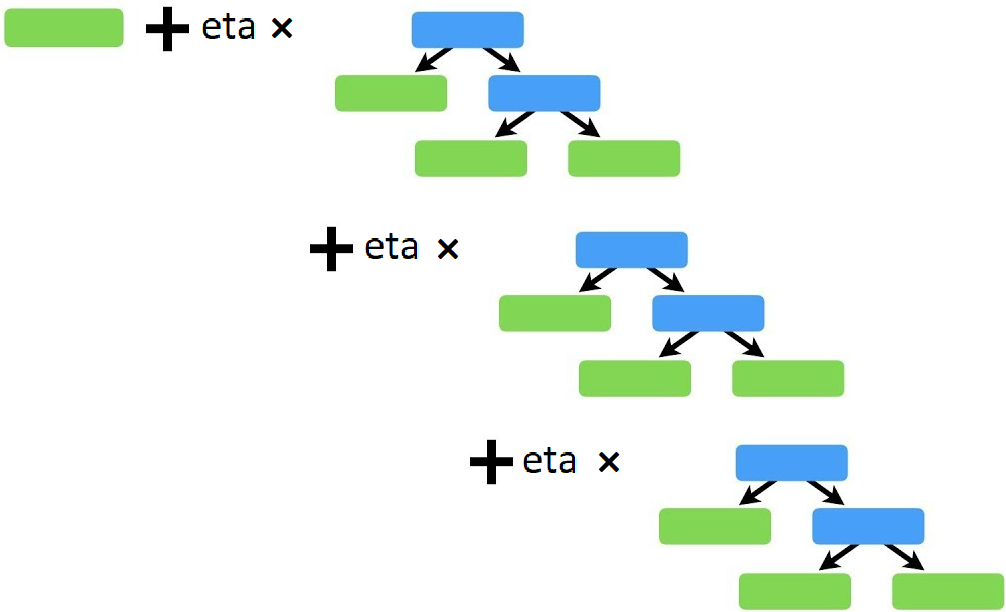
\includegraphics[width=0.8\linewidth,height=0.3\textheight]{figure/xgb} 

}

\caption{XGBoost Çalışma Mantığı}\label{fig:unnamed-chunk-9}
\end{figure}
\hypertarget{nn}{%
\section{Yapay Sinir Ağları}\label{nn}}

Yapay Sinir ağları insan beyninin en temel özelliği olan öğrenme fonksiyonunu gerçekleştiren bilgisayar sistemleridir. Öğrenme işlemini örnekler yardımı ile gerçekleştirirler. Bu ağlar birbirine bağlı yapay sinir hücrelerinden oluşur. Yapay sinir ağları biyolojik sinir sisteminden etkilenerek geliştirilmiştir. Biyolojik sinir hücreleri birbirleri ile sinapsisler vasıtası ile iletişim kurarlar. Bir sinir hücresi işlediği bilgileri Axon'ları yolu ile diğer hücrelere gönderirler (Öztemel, 2003).\\

\begin{figure}

{\centering 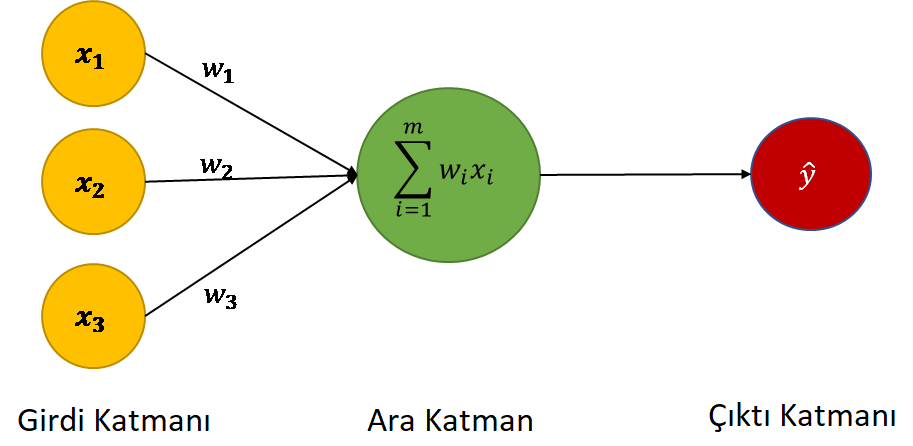
\includegraphics[width=0.8\linewidth,height=0.3\textheight]{figure/basic_neuron} 

}

\caption{Basit Bir Yapay Nöron Örneği (Sahu, 2021)}\label{fig:unnamed-chunk-10}
\end{figure}
Benzer şekilde yapay sinir hücreleri dışarıdan gelen bilgileri bir toplama fonksiyonu ile toplar ve aktivasyon fonksiyonundan geçirerek çıktıyı üretip ağın bağlantılarının üzerinden diğer hücrelere gönderir. Temel bir ağ 3 katmandan meydana gelir;
\begin{itemize}
\item
  Girdi Katmanı
\item
  Ara Katmanlar
\item
  Çıktı Katmanı
\end{itemize}
Her ara katmanın sonunda olabileceği gibi yalnızca çıktı katmanının sonunda da aktivasyon fonksiyonu olabilir. Literatürde en yaygın kullanılan 4 adet aktivasyon fonksiyonu mevcuttur;
\begin{itemize}
\item
  ReLU
\item
  Sigmoid (Lojistik)
\item
  Step
\item
  tanh
\end{itemize}
\begin{figure}

{\centering 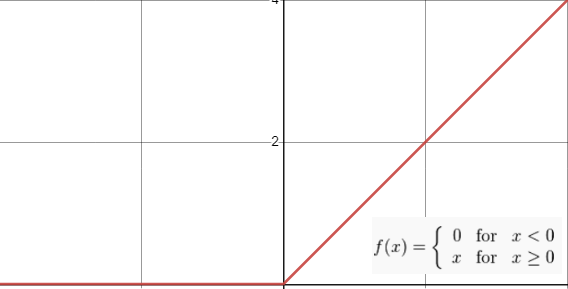
\includegraphics[width=0.49\linewidth,height=0.18\textheight]{figure/relu} 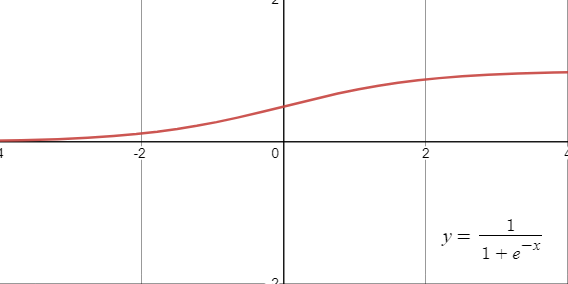
\includegraphics[width=0.49\linewidth,height=0.18\textheight]{figure/sigmoid} 

}

\caption{ReLU ve Sigmoid Fonksiyonu}\label{fig:unnamed-chunk-11}
\end{figure}
\begin{figure}

{\centering 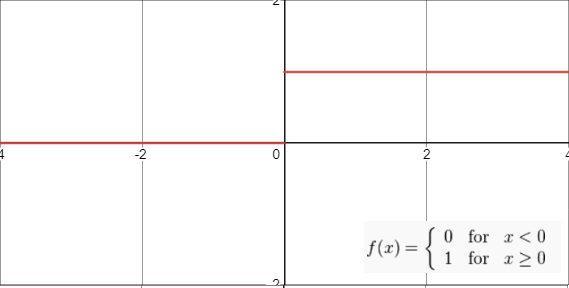
\includegraphics[width=0.49\linewidth,height=0.18\textheight]{figure/step} 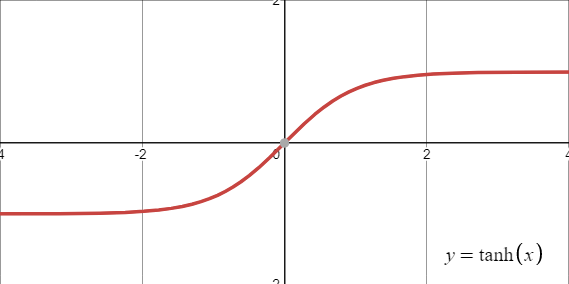
\includegraphics[width=0.49\linewidth,height=0.18\textheight]{figure/tanh} 

}

\caption{Step ve Tanh Fonksiyonu }\label{fig:unnamed-chunk-12}
\end{figure}
\begin{figure}

{\centering 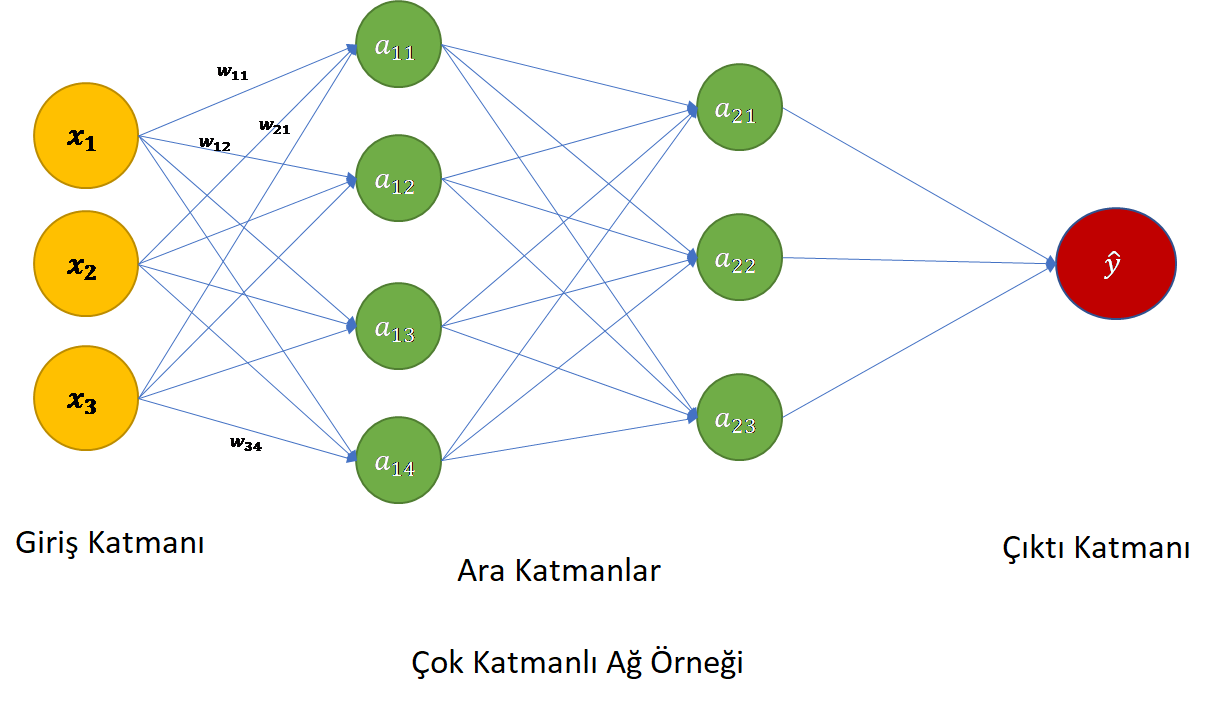
\includegraphics[width=1\linewidth,height=0.3\textheight]{figure/cok_katmanli} 

}

\caption{Çok Katmanlı Yapay Sinir Ağı Örneği (Sahu, 2021)}\label{fig:unnamed-chunk-13}
\end{figure}
~
~

Başlangıçta girdi katmanından alınan verilerin ağırlıkları (weights) rastgele olarak atanır ve ağ çalıştırılır. Çıktı katmanından sonra elde edilen sonuç orijinal verinin bağımlı değişkeni ile en yakın değeri üretene kadar sinir ağı geri yayılım yöntemi ile ağırlıkları optimize etmeye çalışır. Maliyet fonksiyonun türevleri alınarak ağırlıkları optimize etmeyi amaçlayan geri yayılım algoritması orijinal verinin bağımlı değişkeni ile tahmin değeri arasında en düşük hata değerini bulduğu zaman ağın yeni ağırlıklarını son bulduğu ağırlıklar olarak tayin eder.
\begin{figure}

{\centering 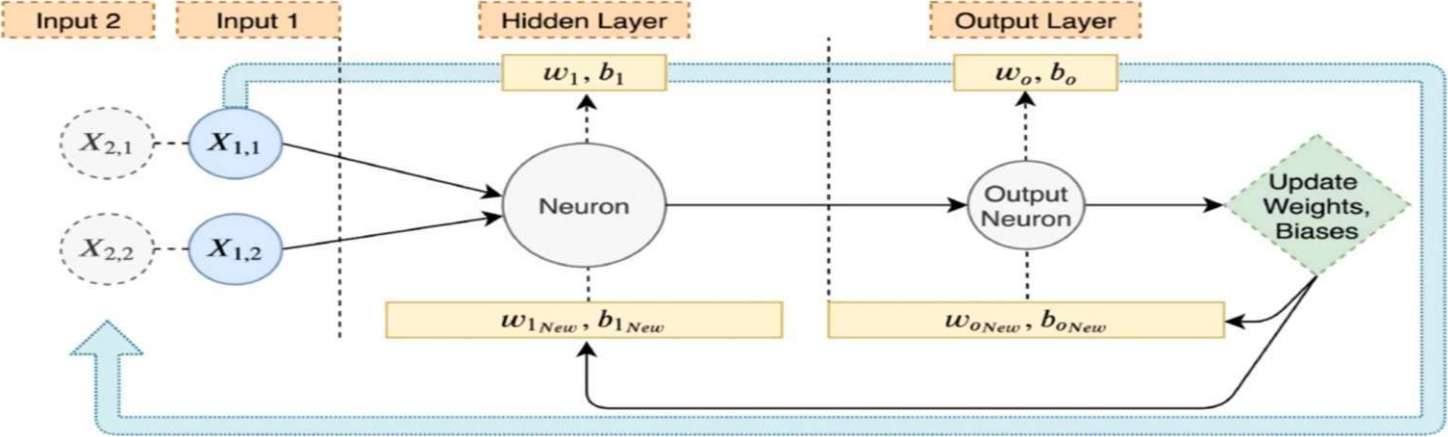
\includegraphics[width=0.85\linewidth,height=0.3\textheight]{figure/geri_yayilim} 

}

\caption{Geri Yaylım Örneği}\label{fig:unnamed-chunk-14}
\end{figure}
Ağın ağırlıkları belirlendikten sonra her bir ağırlığın ne anlama geldiği bilinmemektedir. Bu nedenle yapay sinir ağlarına ``kara kutu'' yakıştırması yapılmaktadır. Ağın performansını etkileyen bağlıca faktörler kullanılan aktivasyon fonksiyonu, öğrenme stratejisi ve öğrenme kuralıdır (Öztemel, 2003).

\hypertarget{uygulama}{%
\chapter{Uygulama}\label{uygulama}}

Bu bölümde yapılan uygulama sunulmuştur.\\
\hspace*{0.333em}

Uygulamada kullanılan veriler 2021 yılında Güney Kore'de yapılan bir araştırmadan alınmıştır (Park ve diğerleri, 2021). Uzmanlar tarafından yapılan tetkikler ile her bir hasta için (her bir el için) ciddiyet sınıflandırılması mild, moderate, severe olarak belirlenmiştir. Çalışmada 1037 elden alınan verilerin 405 (39.05\%) adedi erkek hastalardan, 632 (60.95\%) adedi kadın hastalardan elde edilmiştir. Uzmanlar tarafından 1037 adet elin, 507 (48.9\%) adedi mild, 276 (26.6\%) adedi moderate ve 254 (24.5\%) adedi severe olarak sınıflandırılmıştır.

Araştırmada uzman hekimler tarafından hastalara yöneltilen sorular ile şikayetleri olan ellerine ilişkin aşağıdaki değişkenler için veri toplanmıştır;
\begin{itemize}
\item
  Hands (Eller)
\item
  Age (Yaş)
\item
  Sex (Cinsiyet)
\item
  BMI (Body-mass index, Vücut kitle indeksi)
\item
  Side (Right side involvement, Sağ Elde Bulgu)
\item
  Diabetes (Diyabet Hastalığı Durumu)
\item
  Duration (Duration in months, Dayanma süresi (Aylık))
\item
  NRS (Numeric rating scale of pain, Hissedilen acının numerik karşılığı)
\item
  NP (Noctural Pain, Gece Ağrıları)
\item
  Weakness (Tenar weakness and/or atrophy, Avuç İçi Zayıflık ve/veya Körelme)
\item
  CSA (Cyclosporine dosage in \(mm^2\), Siklosporin dozu (\(mm^2\)))
\item
  PB (fexor retinaculum in mm, Fleksör retinakulum (mm))
\end{itemize}
\begin{longtable}[]{@{}lr@{}}
\caption{\label{tab:overall} Sayısal Değişkenlerin Tanımlayıcı İstatistikleri}\tabularnewline
\toprule
& Overall \\
\midrule
\endfirsthead
\toprule
& Overall \\
\midrule
\endhead
Age,years (mean \(\pm\) SD) & 58 \(\pm\) 10.8 \\
BMI, kg/m\(^2\) (mean \(\pm\) SD) & 24.8 \(\pm\) 3.4 \\
Duration, months (mean \(\pm\) SD) & 8.3 \(\pm\) 9.6 \\
NRS (mean \(\pm\) SD) & 4.4 \(\pm\) 1.8 \\
CSA, mm\(^2\) (mean \(\pm\) SD) & 15.2 \(\pm\) 4.3 \\
PB, mm (mean \(\pm\) SD) & 2.5 \(\pm\) 1.8 \\
\bottomrule
\end{longtable}
\begin{longtable}[]{@{}lrrrr@{}}
\caption{\label{tab:sayisal} Değişkenlerin Bağımlı Değişkene Göre Tanımlayıcı İstatistikleri \footnotesize (P-Value Değerleri Tek Yönlü Varyans Analiz Testi ile Elde Edilmiştir.)}\tabularnewline
\toprule
& Mild & Moderate & Severe & P Value \\
\midrule
\endfirsthead
\toprule
& Mild & Moderate & Severe & P Value \\
\midrule
\endhead
Age,years (mean \(\pm\) SD) & 57.3 \(\pm\) 10.6 & 59.2 \(\pm\) 10.8 & 57.8 \(\pm\) 11.2 & 0.069 \\
BMI, kg/m\(^2\) (mean \(\pm\) SD) & 24.2 \(\pm\) 3.4 & 24.7 \(\pm\) 3 & 25.8 \(\pm\) 3.7 & 0 \\
Duration, months (mean \(\pm\) SD) & 4.3 \(\pm\) 5 & 8.5 \(\pm\) 8.2 & 15.9 \(\pm\) 12.8 & 0 \\
NRS (mean \(\pm\) SD) & 3.3 \(\pm\) 1.3 & 4.9 \(\pm\) 1.5 & 6.1 \(\pm\) 1.5 & 0 \\
CSA, mm\(^2\) (mean \(\pm\) SD) & 13.2 \(\pm\) 3 & 15.4 \(\pm\) 3.2 & 18.9 \(\pm\) 5 & 0 \\
PB, mm (mean \(\pm\) SD) & 2.1 \(\pm\) 0.8 & 2.6 \(\pm\) 2.4 & 3.1 \(\pm\) 2.3 & 0 \\
\bottomrule
\end{longtable}
\hfill\break
\hfill\break
~
\begin{longtable}[]{@{}lrrrr@{}}
\caption{\label{tab:catvar} Katagorik Değişkenlerin Bağımlı Değişkence Frekans Dağılımı \footnotesize (P-Value Değerleri Ki-Kare Bağımsızlık Testi ile Elde Edilmiştir.)}\tabularnewline
\toprule
& Mild & Moderate & Severe & P value \\
\midrule
\endfirsthead
\toprule
& Mild & Moderate & Severe & P value \\
\midrule
\endhead
Eller, n (\%) & 507 (48.9) & 276 (26.6) & 254 (24.5) & - \\
Cinsiyet (Kadın), n (\%) & 308 (60.7) & 153 (55.4) & 171 (67.3) & 0.02 \\
Sağ Elde Bulgu, n (\%) & 243 (47.9) & 149 (54) & 119 (46.9) & 0.181 \\
Diyabet, n (\%) & 47 (9.3) & 45 (16.3) & 54 (21.3) & 0 \\
Gece Ağrıları, n (\%) & 102 (20.1) & 142 (51.4) & 212 (83.5) & 0 \\
Avuç İçi Zayıflık ve/veya Körelme, n (\%) & 1 (0.2) & 24 (8.7) & 169 (66.5) & 0 \\
\bottomrule
\end{longtable}
Kullanılan verilere ait tanımlayıcı istatistikler Tablo \ref{tab:overall}, Tablo \ref{tab:sayisal} ve Tablo \ref{tab:catvar} de verilmiştir. Varsayım kontrollerinin ardından sayısal değişkenlerin ciddiyet sınıflarına göre farklılık gösterip göstermediği tek yönlü varyans analizi ile araştırılmıştır (\(\alpha = 0.05\)). Tablo \ref{tab:sayisal}'de yer alan P-Value değerleri incelendiğinde ciddiyet sınıflamasının yaşa göre anlamlı bir değişim göstermediği diğer tüm değişkenler için anlamlı bir fark olduğu görülmüştür.

Tablo \ref{tab:catvar}'de yer alan P-Value değerleri incelendiğinde ciddiyet sınıflamasının KTS'nin sağ veya sol elde görülmesine göre anlamlı bir değişim göstermediği diğer tüm değişkenler için anlamlı bir fark olduğu görülmüştür.

~
~

Bu çalışmada, KTS ciddiyet sınıflandırması için K-En Yakın Komşuluk, Rassal Ormanlar, Yapay Sinir Ağları ve XGBoost yöntemleri kullanılmıştır.\\
İlk olarak orijinal verilerdeki 3 sınıf (Mild, Moderate, Severe) için sınıflandırma hedeflenmiştir.\\
Bölüm \ref{multiclass}'de bu problem için farklı modeller ile elde edilen sonuçlara yer verilmiştir.\\
Uygulamanın ikinci bölümünde hedef değişken iki sınıfa indirgenmiş ve bu probleme ait sonuçlar bölüm \ref{binary}'de paylaşılmıştır.\\
Uygulamada Python programlama dili ve Scikit-Learn, Pandas, Numpy, Matplotlib,XGBoost kütüphanelerinden yararlanılmıştır.\\
Bu bölümde modellerin performanslarını değerlendirmek üzere kesinlik, duyarlılık, F1-skoru, doğruluk oranı, dengelenmiş doğruluk oranı hesaplanmıştır.

\hypertarget{multiclass}{%
\section{Çok Sınıflı(Multiclass) Sınıflama Problemi}\label{multiclass}}

Bu bölümde KTS ciddiyet sınıflandırması için hedef değişkenin 3 farklı ciddiyet düzeyine sahip olduğu durumda farklı sınıflama algoritmaları ile ciddiyet düzeyinin tahminlenmesi amaçlanmıştır.

\hypertarget{mult_knn}{%
\subsection{K-En Yakın Komşuluk Modeli}\label{mult_knn}}

Bu bölümde veri seti üzerinde K - En yakın komşuluk modeli kullanılmış ve çıktıları değerlendirilmiştir.

\hypertarget{hiper-parametre-seuxe7imi}{%
\subsubsection{Hiper Parametre Seçimi}\label{hiper-parametre-seuxe7imi}}

Daha önce belirlenen parametre uzayını ve Scikit-Learn kütüphanesinde bulunan GridSearchCV algoritması ile en yüksek doğruluk oranı yakalanana kadar çalışması sağlanmıştır.
\begin{figure}

{\centering 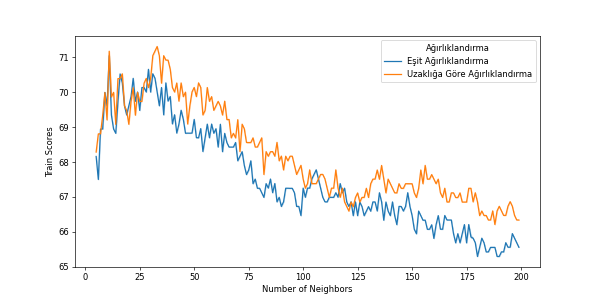
\includegraphics[width=1.1\linewidth,height=0.55\textheight]{figure/KNN_Grid_Graph} 

}

\caption{Üç Sınıflı K-NN Eğitim Verisi Doğruluk Skorları}\label{fig:unnamed-chunk-21}
\end{figure}
K-En yakın komşuluk modeli için en yüksek doğruluk oranı aşağıdaki parametreler ile bulunmuştur;
\begin{itemize}
\tightlist
\item
  `algorithm':`auto'
\item
  `n\_neighbors':33
\item
  `weights':`distance'
\end{itemize}
\newpage

\hypertarget{en-iyi-parametreli-model}{%
\subsubsection{En İyi Parametreli Model}\label{en-iyi-parametreli-model}}

Bulunan parametrelerle kurulan modelin sınıflandırma metrikleri aşağıdaki gibidir.
\begin{verbatim}
              precision    recall  f1-score   support

        Mild       0.76      0.92      0.83       137
    Moderate       0.51      0.42      0.46        65
      Severe       0.89      0.68      0.77        72

    accuracy                           0.74       274
   macro avg       0.72      0.67      0.69       274
weighted avg       0.73      0.74      0.73       274
\end{verbatim}
\begin{verbatim}
Balanced Accuracy Score : 0.6718827333790838
\end{verbatim}
\begin{figure}

{\centering 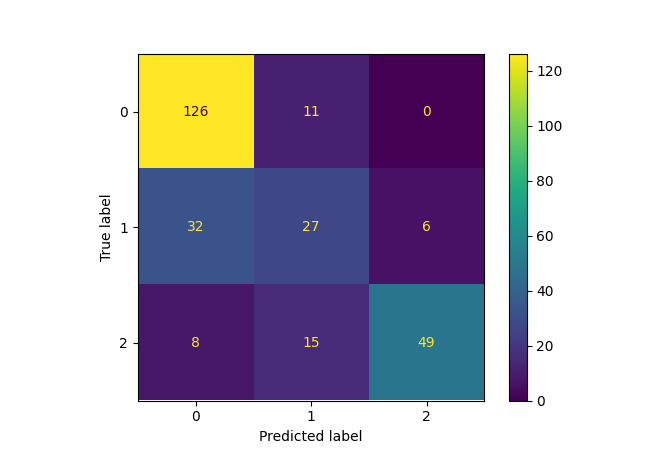
\includegraphics[width=1.05\linewidth,height=0.6\textheight]{figure/knn_conf} 

}

\caption{Üç Sınıflı K-NN Modeli Karmaşıklık Matrisi}\label{fig:unnamed-chunk-26}
\end{figure}
\begin{figure}

{\centering 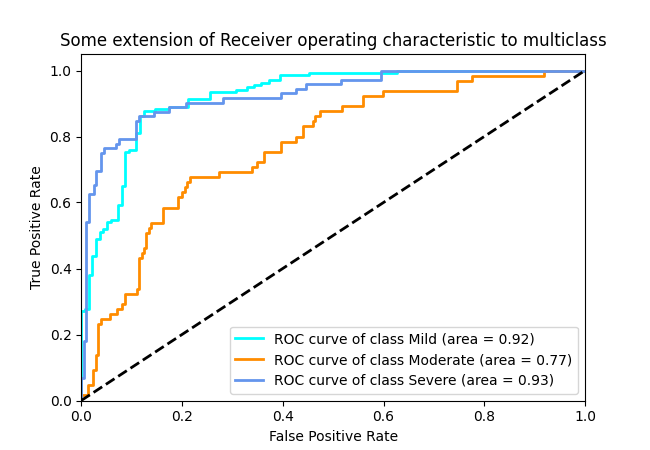
\includegraphics[width=1.05\linewidth,height=0.6\textheight]{figure/roc_curve_KNeighborsClassifier} 

}

\caption{Üç Sınıflı K-NN Modeli ROC Eğrisi ve AUC Değerleri}\label{fig:unnamed-chunk-27}
\end{figure}
\hypertarget{mult_rf}{%
\subsection{Rassal Ormanlar Modeli}\label{mult_rf}}

Bu bölümde veri seti üzerinde rassal ormanlar modeli kullanılmış ve çıktıları değerlendirilmiştir.

\hypertarget{hiper-parametre-seuxe7imi-1}{%
\subsubsection{Hiper Parametre Seçimi}\label{hiper-parametre-seuxe7imi-1}}

Daha önce belirlenen parametre uzayını ve Scikit-Learn kütüphanesinde bulunan GridSearchCV algoritması ile en yüksek doğruluk oranı yakalanana kadar çalışması sağlanmıştır.
\begin{figure}

{\centering 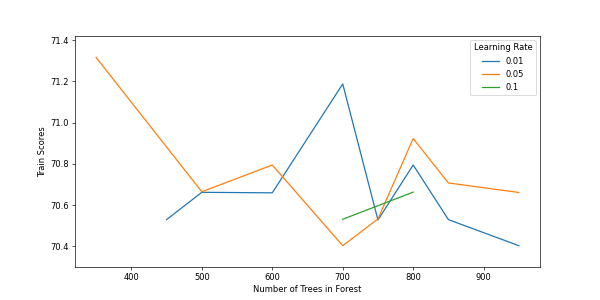
\includegraphics[width=1.1\linewidth,height=0.5\textheight]{figure/RF_Grid_Graph} 

}

\caption{Üç Sınıflı Rassal Ormanlar Modeli Eğitim Verisi Doğruluk Skorları}\label{fig:unnamed-chunk-29}
\end{figure}
Rassal ormanlar modeli için en yüksek doğruluk oranı aşağıdaki parametreler ile bulunmuştur;
\begin{itemize}
\tightlist
\item
  `ccp\_alpha':0.05
\item
  `criterion':`gini'
\item
  `weights':`distance'
\item
  `max\_features':`auto'
\item
  `max\_samples':10
\item
  `n\_estimators':350
\end{itemize}
\newpage

\hypertarget{en-iyi-parametreli-model-1}{%
\subsubsection{En İyi Parametreli Model}\label{en-iyi-parametreli-model-1}}

Bulunan parametrelerle kurulan modelin sınıflandırma metrikleri aşağıdaki gibidir.
\begin{verbatim}
              precision    recall  f1-score   support

        Mild       0.73      0.99      0.84       137
    Moderate       0.58      0.34      0.43        65
      Severe       0.94      0.68      0.79        72

    accuracy                           0.75       274
   macro avg       0.75      0.67      0.69       274
weighted avg       0.75      0.75      0.73       274
\end{verbatim}
\begin{verbatim}
Balanced Accuracy Score : 0.6681395179570361
\end{verbatim}
\begin{figure}

{\centering 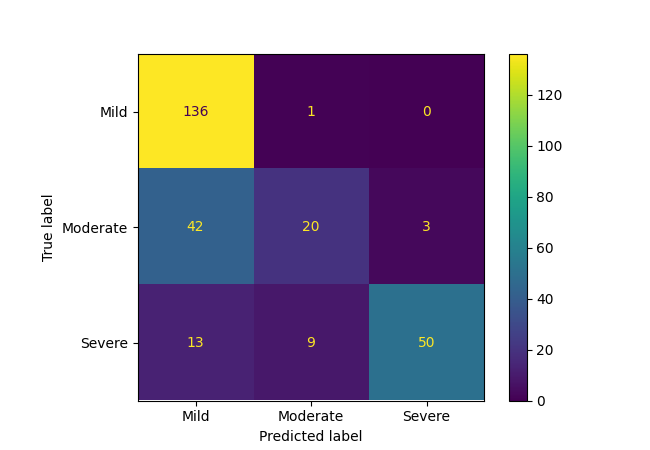
\includegraphics[width=1.05\linewidth,height=0.6\textheight]{figure/rfc_conf} 

}

\caption{Üç Sınıflı Rassal Ormanlar Modeli Karmaşıklık Matrisi}\label{fig:unnamed-chunk-34}
\end{figure}
\begin{figure}

{\centering 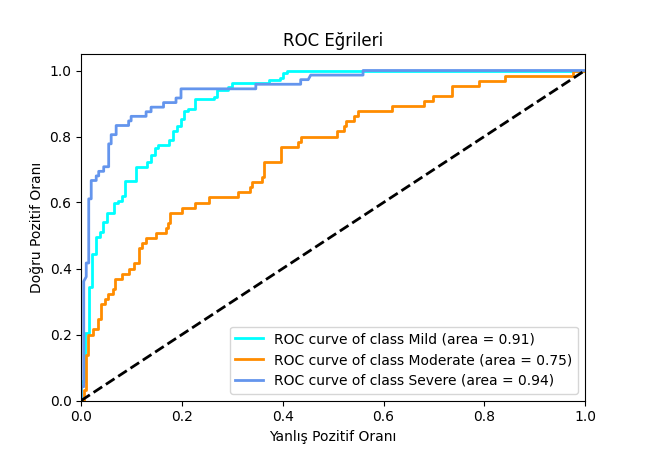
\includegraphics[width=1.05\linewidth,height=0.6\textheight]{figure/roc_curve_RandomForestClassifier} 

}

\caption{Üç Sınıflı Rassal Ormanlar Modeli ROC Eğrisi ve AUC Değerleri}\label{fig:unnamed-chunk-35}
\end{figure}
\hypertarget{mult_xgb}{%
\subsection{eXtreme Gradient Boosting (XGBoost)}\label{mult_xgb}}

Bu bölümde veri seti üzerinde XGBoost modeli kullanılmış ve çıktıları değerlendirilmiştir.

\hypertarget{hiper-parametre-seuxe7imi-2}{%
\subsubsection{Hiper Parametre Seçimi}\label{hiper-parametre-seuxe7imi-2}}

Daha önce belirlenen parametre uzayını ve Scikit-Learn kütüphanesinde bulunan GridSearchCV algoritması ile en yüksek doğruluk oranı yakalanana kadar çalışması sağlanmıştır.
\begin{figure}

{\centering 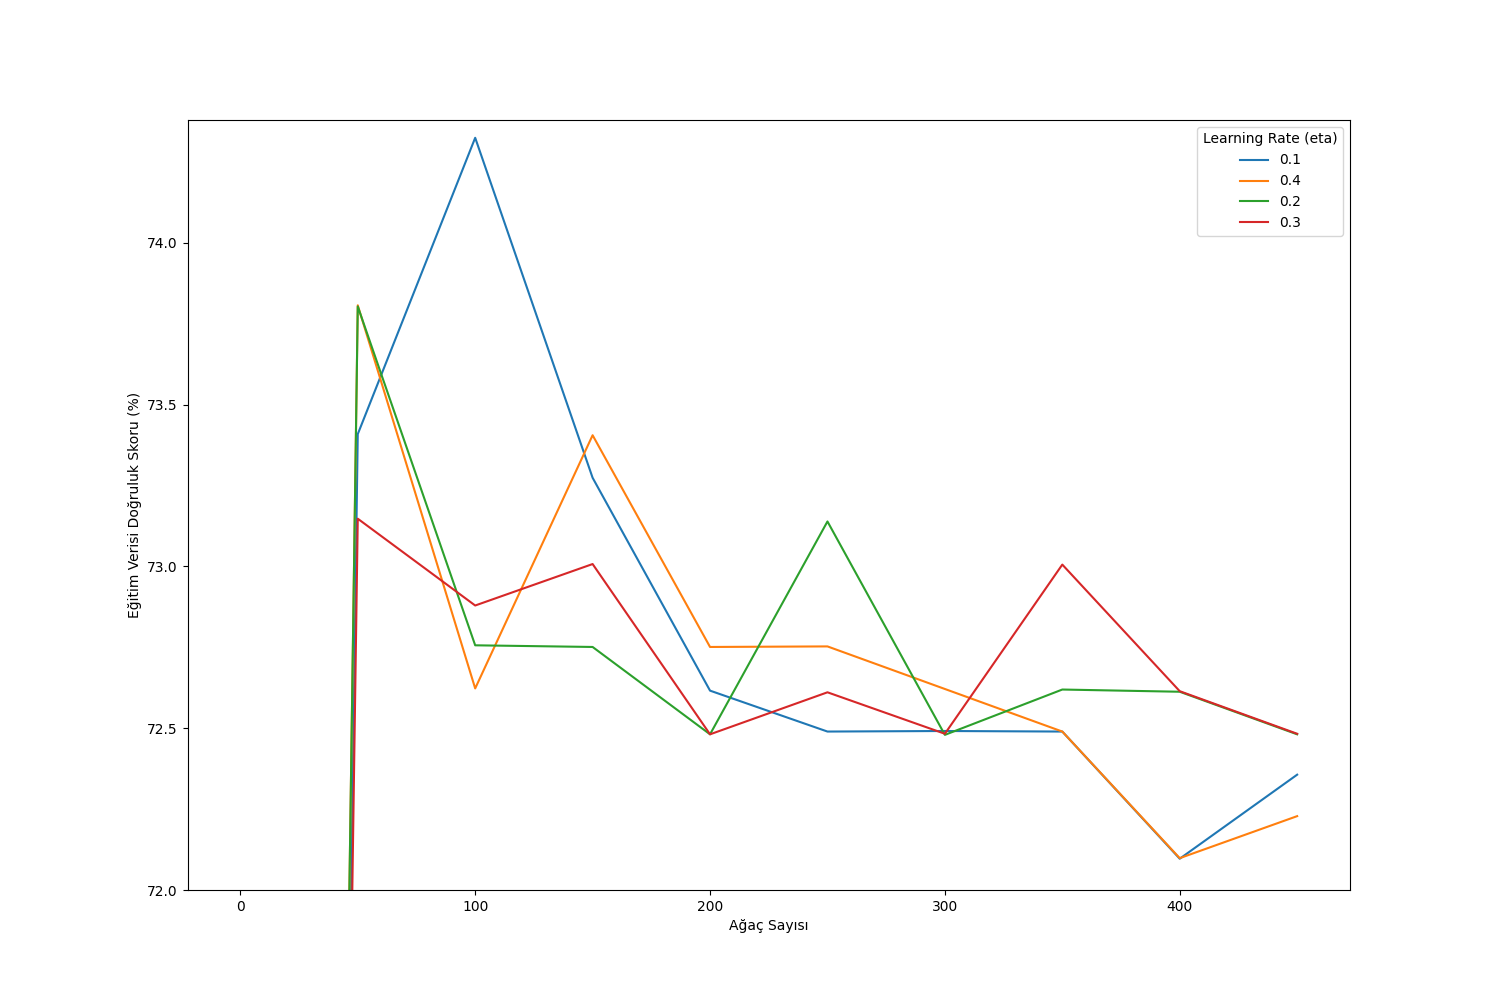
\includegraphics[width=1.1\linewidth,height=0.5\textheight]{figure/XGB_Grid_Graph} 

}

\caption{Üç Sınıflı XGBoost Modeli Eğitim Verisi Doğruluk Skorları}\label{fig:unnamed-chunk-37}
\end{figure}
XGBoost modeli için en yüksek doğruluk oranı aşağıdaki parametreler ile bulunmuştur;
\begin{itemize}
\tightlist
\item
  `eta':0.1
\item
  `max\_depth':3
\item
  `min\_child\_weight':10
\item
  `n\_estimators':100
\item
  `objective':`multi:softprob'
\item
  `sumsample':0.5
\end{itemize}
\newpage

Bulunan parametrelerle kurulan modelin sınıflandırma metrikleri aşağıdaki gibidir.
\begin{verbatim}
              precision    recall  f1-score   support

        Mild       0.80      0.89      0.84       137
    Moderate       0.60      0.57      0.58        65
      Severe       0.90      0.74      0.81        72

    accuracy                           0.77       274
   macro avg       0.76      0.73      0.74       274
weighted avg       0.78      0.77      0.77       274
\end{verbatim}
\begin{verbatim}
Balanced Accuracy Score : 0.7319509430823299
\end{verbatim}
\begin{figure}

{\centering 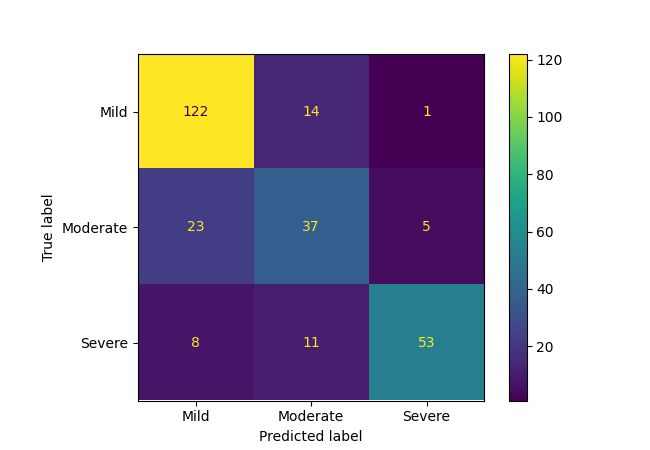
\includegraphics[width=1.05\linewidth,height=0.6\textheight]{figure/xgb_conf} 

}

\caption{Üç Sınıflı XGBoost Modeli Karmaşıklık Matrisi}\label{fig:unnamed-chunk-42}
\end{figure}
\begin{figure}

{\centering 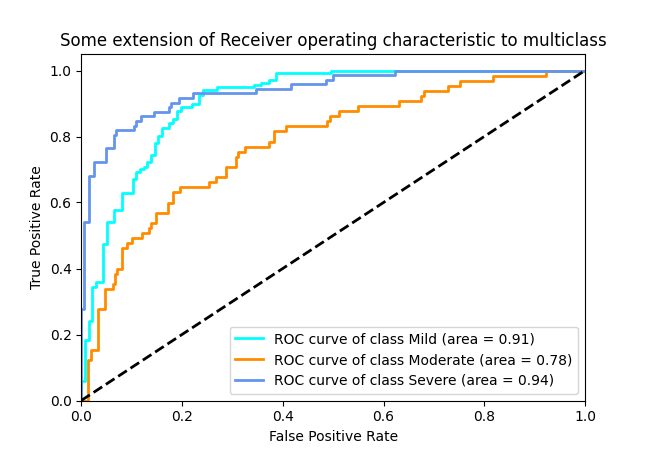
\includegraphics[width=1.05\linewidth,height=0.6\textheight]{figure/roc_curve_XGBClassifier} 

}

\caption{Üç Sınıflı XGBoost Modeli ROC Eğrisi ve AUC Değerleri}\label{fig:unnamed-chunk-43}
\end{figure}
\hypertarget{mult_nn}{%
\subsection{Yapay Sinir Ağları (Neural Networks)}\label{mult_nn}}

Bu bölümde veri seti üzerinde yapay sinir ağları modeli kullanılmış ve çıktıları değerlendirilmiştir.

\hypertarget{hiper-parametre-seuxe7imi-3}{%
\subsubsection{Hiper Parametre Seçimi}\label{hiper-parametre-seuxe7imi-3}}

Daha önce belirlenen parametre uzayını ve Scikit-Learn kütüphanesinde bulunan GridSearchCV algoritması ile en yüksek doğruluk oranı yakalanana kadar çalışması sağlanmıştır.
\begin{figure}

{\centering 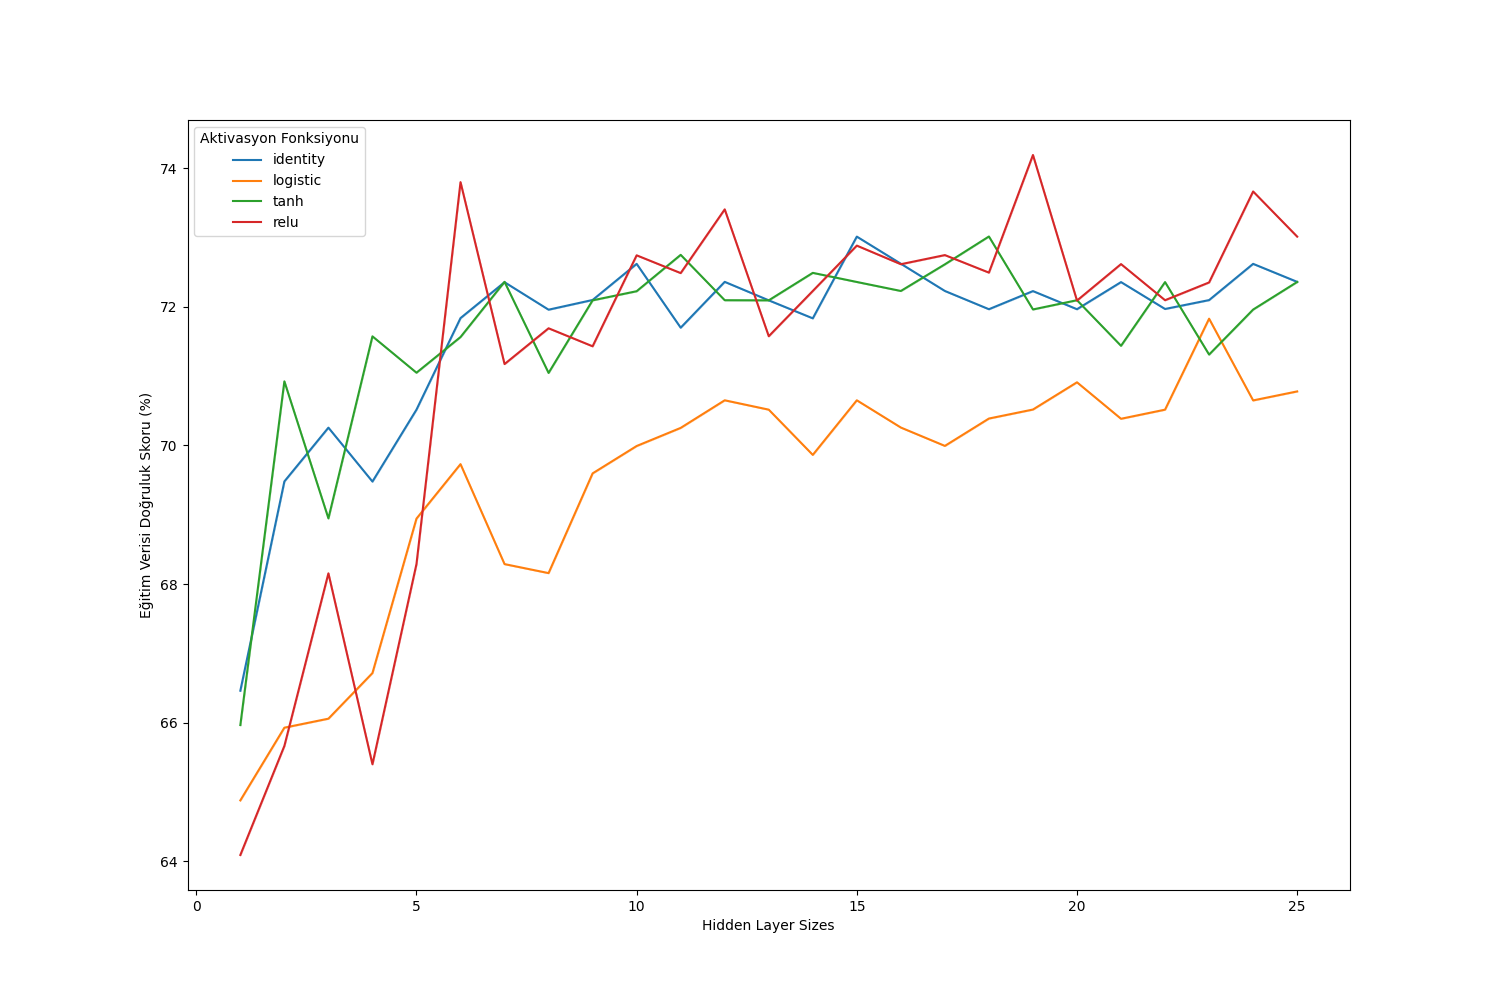
\includegraphics[width=1.1\linewidth,height=0.5\textheight]{figure/NN_Grid_Graph} 

}

\caption{Üç Sınıflı Yapay Sinir Ağları Modeli Eğitim Verisi Doğruluk Skorları}\label{fig:unnamed-chunk-45}
\end{figure}
Yapay sinir ağları modeli için en yüksek doğruluk oranı aşağıdaki parametreler ile bulunmuştur;
\begin{itemize}
\tightlist
\item
  `activation':`relu'
\item
  'hidden\_layer\_sizes:19
\item
  `learning\_rate':`adaptive'
\end{itemize}
\newpage

Bulunan parametrelerle kurulan modelin sınıflandırma metrikleri aşağıdaki gibidir.
\begin{verbatim}
              precision    recall  f1-score   support

        Mild       0.83      0.87      0.85       137
    Moderate       0.51      0.58      0.55        65
      Severe       0.89      0.71      0.79        72

    accuracy                           0.76       274
   macro avg       0.75      0.72      0.73       274
weighted avg       0.77      0.76      0.76       274
\end{verbatim}
\begin{verbatim}
Balanced Accuracy Score : 0.7205206188782832
\end{verbatim}
\begin{figure}

{\centering 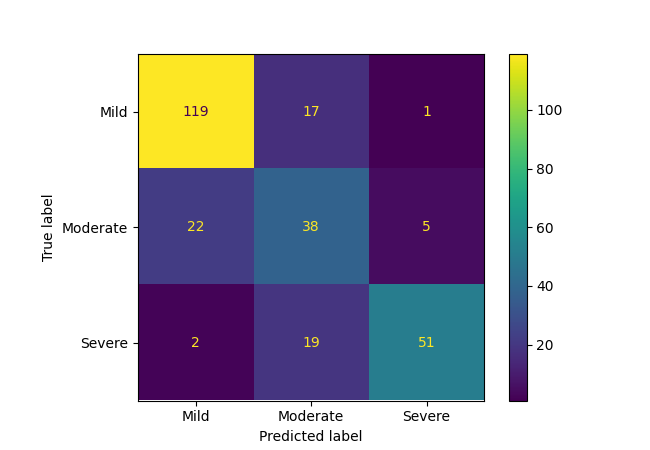
\includegraphics[width=1.05\linewidth,height=0.6\textheight]{figure/nn_conf} 

}

\caption{Üç Sınıflı Yapay Sinir Ağları Modeli Karmaşıklık Matrisi}\label{fig:unnamed-chunk-50}
\end{figure}
\begin{figure}

{\centering 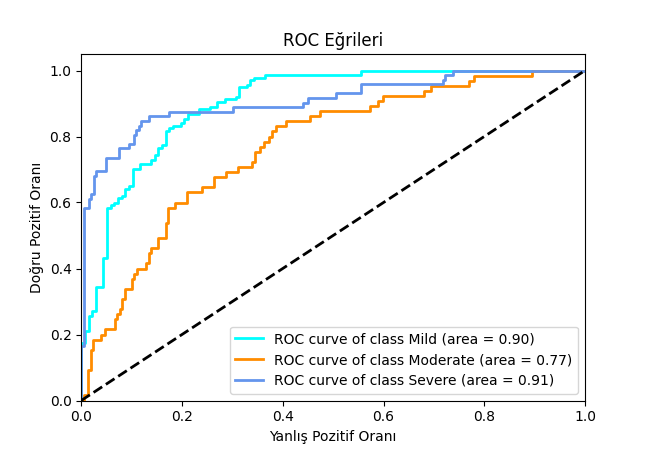
\includegraphics[width=1.05\linewidth,height=0.6\textheight]{figure/roc_curve_MLPClassifier} 

}

\caption{Üç Sınıflı Yapay Sinir Ağları Modeli ROC Eğrisi ve AUC Değerleri}\label{fig:unnamed-chunk-51}
\end{figure}
\hypertarget{uxe7ok-sux131nux131flux131-sux131nux131flama-probleminin-modellerinin-deux11ferlendirdirilmesi}{%
\subsection{Çok Sınıflı Sınıflama Probleminin Modellerinin Değerlendirdirilmesi}\label{uxe7ok-sux131nux131flux131-sux131nux131flama-probleminin-modellerinin-deux11ferlendirdirilmesi}}

Bölüm \ref{mult_knn}, \ref{mult_rf}, \ref{mult_xgb} ve \ref{mult_nn}`den elde edilen sonuçlar incelenmiş olup, üç sınıflı problem için \%77 doğru sınıflama oranı ile en iyi model XGBoost olarak bulunmuştur.\\
Bölüm \ref{mult_xgb}'de bulunan performans metrikleri yakından incelendiğinde, duyarlılık metriği 'Moderate' ve `Severe' sınıfları için `Mild' sınıfına kıyasla daha düşük kalmıştır.\\
Duyarlılık metriğindeki düşüklüğün sebep olabileceği yanlış sınıflandırmaların önüne geçebilmek amacı ile bölüm \ref{binary}'de problem iki sınıflı probleme indirgenecek ve modeller tekrar çalıştırılacaktır.

\hypertarget{binary}{%
\section{İki Sınıflı Sınıflama}\label{binary}}

Bu bölümde KTS ciddiyet sınıflandırması için hedef değişkenin 3 farklı ciddiyet düzeyine sahip olduğu veri seti `Moderate' ve `Severe' ciddiyet düzeyleri birleştirilerek problemin 2 farklı ciddiyet düzeyine indirgenip farklı sınıflama algoritmaları ile ciddiyet düzeyinin tahminlenmesi amaçlanmıştır.

\hypertarget{bin_knn}{%
\subsection{K-En Yakın Komşuluk Modeli}\label{bin_knn}}

Bu bölümde veri seti üzerinde K - En yakın komşuluk modeli kullanılmış ve çıktıları değerlendirilmiştir.

\hypertarget{hiper-parametre-seuxe7imi-4}{%
\subsubsection{Hiper Parametre Seçimi}\label{hiper-parametre-seuxe7imi-4}}

Daha önce belirlenen parametre uzayını ve Scikit-Learn kütüphanesinde bulunan GridSearchCV algoritması ile en yüksek doğruluk oranı yakalanana kadar çalışması sağlanmıştır.
\begin{figure}

{\centering 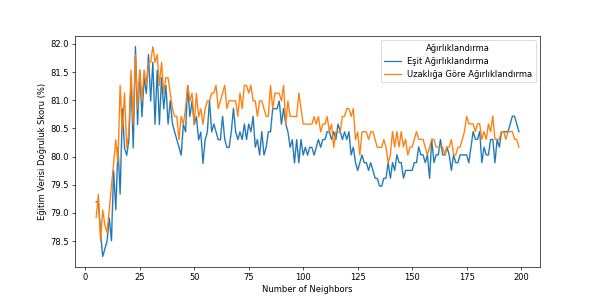
\includegraphics[width=1.1\linewidth,height=0.55\textheight]{figure/KNN_bin_Grid_Graph} 

}

\caption{İki Sınıflı K-NN Modeli Eğitim Verisi Doğruluk Skorları}\label{fig:unnamed-chunk-54}
\end{figure}
\newpage

K-En yakın komşuluk modeli için en yüksek doğruluk oranı aşağıdaki parametreler ile bulunmuştur;
\begin{itemize}
\tightlist
\item
  `algorithm':`auto'\\
\item
  `n\_neighbors':23\\
\item
  `weights':`uniform'
\end{itemize}
\hypertarget{en-iyi-parametreli-model-2}{%
\subsubsection{En İyi Parametreli Model}\label{en-iyi-parametreli-model-2}}

Bulunan parametrelerle kurulan modelin sınıflandırma metrikleri aşağıdaki gibidir.
\begin{verbatim}
              precision    recall  f1-score   support

        Mild       0.77      0.88      0.82       153
     Mod+Sev       0.87      0.75      0.80       159

    accuracy                           0.81       312
   macro avg       0.82      0.82      0.81       312
weighted avg       0.82      0.81      0.81       312
\end{verbatim}
\begin{verbatim}
Balanced Accuracy Score : 0.8153903070662227
\end{verbatim}
\begin{figure}

{\centering 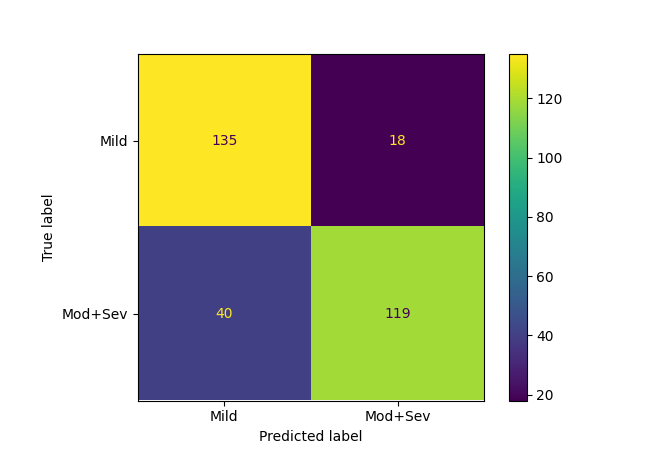
\includegraphics[width=1.05\linewidth,height=0.6\textheight]{figure/knn_bin_conf} 

}

\caption{İki Sınıflı K-NN Modeli Karmaşıklık Matrisi}\label{fig:unnamed-chunk-59}
\end{figure}
\begin{figure}

{\centering 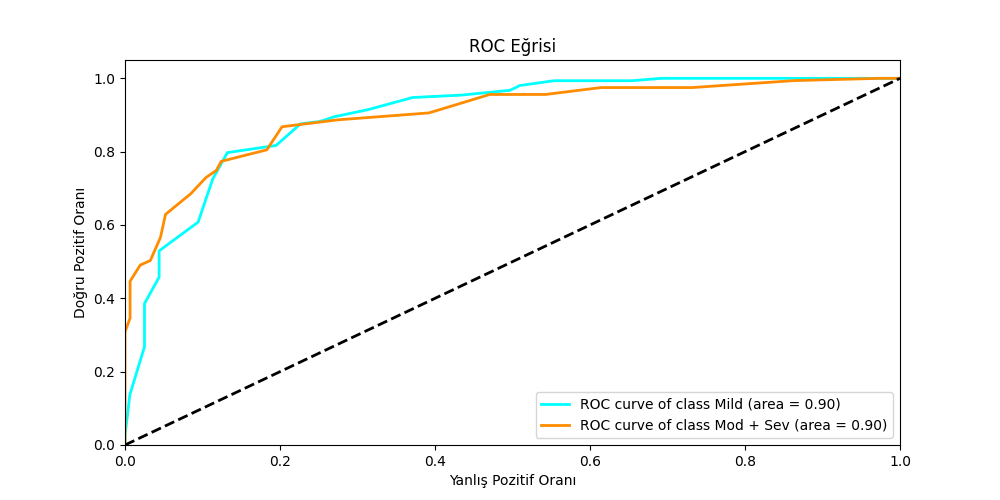
\includegraphics[width=1.05\linewidth,height=0.6\textheight]{figure/KNeighborsClassifier_binary_roc} 

}

\caption{İki Sınıflı K-NN Modeli ROC Eğrisi ve AUC Değerleri}\label{fig:unnamed-chunk-60}
\end{figure}
\hypertarget{bin_rf}{%
\subsection{Rassal Ormanlar Modeli}\label{bin_rf}}

Bu bölümde veri seti üzerinde rassal ormanlar modeli kullanılmış ve çıktıları değerlendirilmiştir.

\hypertarget{hiper-parametre-seuxe7imi-5}{%
\subsubsection{Hiper Parametre Seçimi}\label{hiper-parametre-seuxe7imi-5}}

Daha önce belirlenen parametre uzayını ve Scikit-Learn kütüphanesinde bulunan GridSearchCV algoritması ile en yüksek doğruluk oranı yakalanana kadar çalışması sağlanmıştır.
\begin{figure}

{\centering 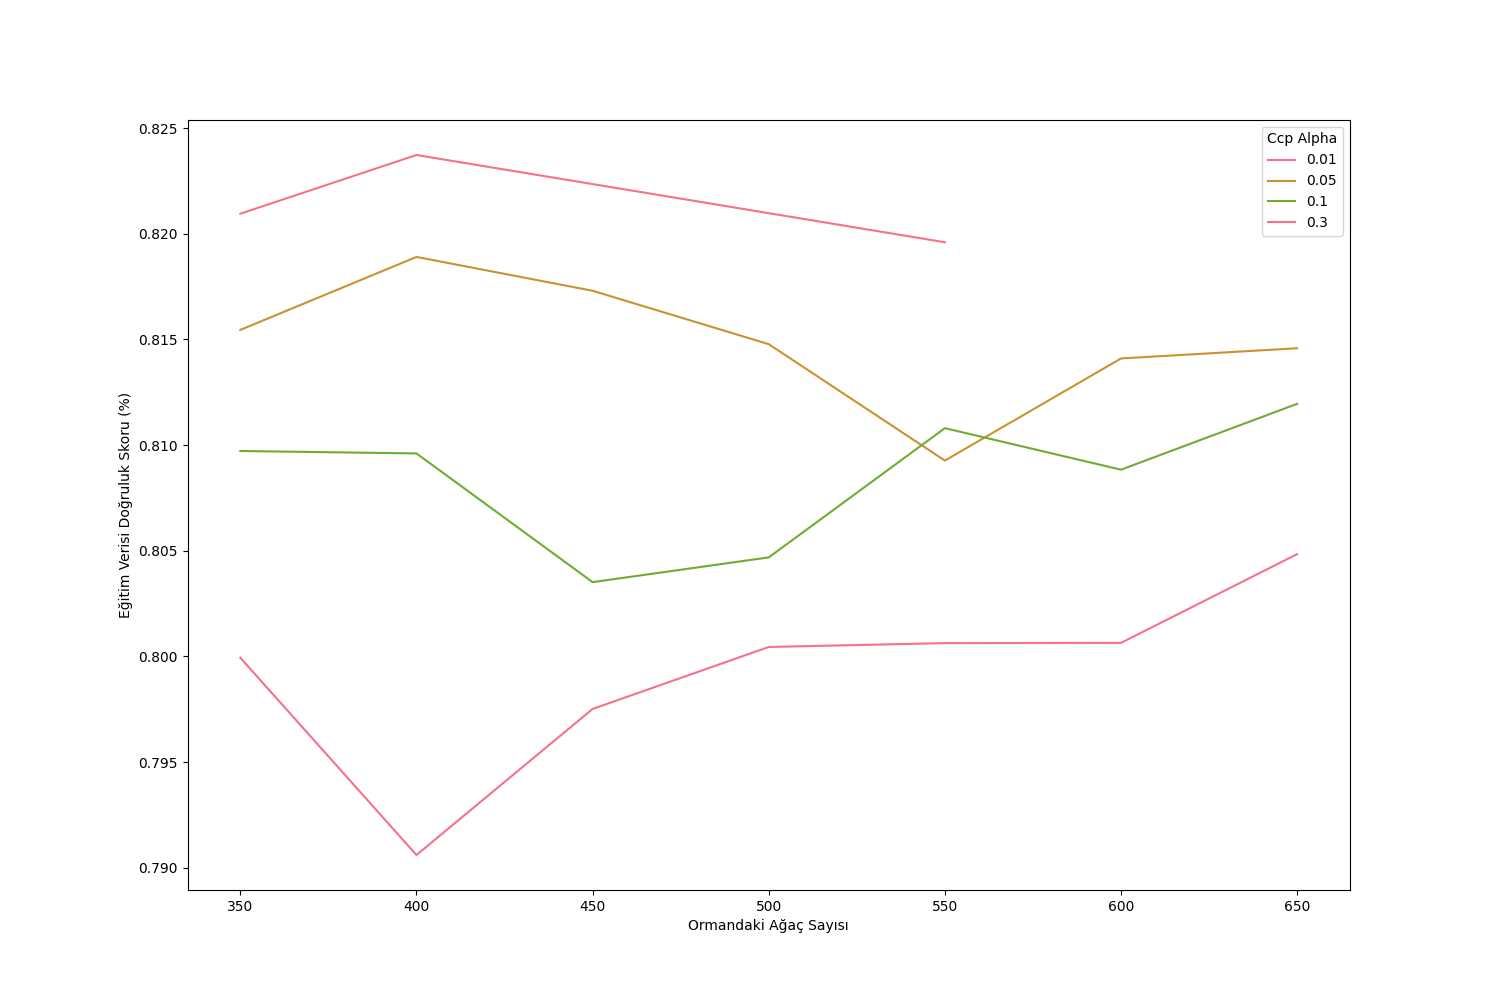
\includegraphics[width=1.1\linewidth,height=0.55\textheight]{figure/RF_bin_Grid_Graph} 

}

\caption{İki Sınıflı Rassal Ormanlar Modeli Eğitim Verisi Doğruluk Skorları}\label{fig:unnamed-chunk-62}
\end{figure}
Rassal ormanlar modeli için en yüksek doğruluk oranı aşağıdaki parametreler ile bulunmuştur;
\begin{itemize}
\tightlist
\item
  `ccp\_alpha': 0.01\\
\item
  `max\_features': `auto'\\
\item
  `max\_samples': 10\\
\item
  `n\_estimators': 400\\
  \newpage  
\end{itemize}
\hypertarget{en-iyi-parametreli-model-3}{%
\subsubsection{En İyi Parametreli Model}\label{en-iyi-parametreli-model-3}}

Bulunan parametrelerle kurulan modelin sınıflandırma metrikleri aşağıdaki gibidir.
\begin{verbatim}
              precision    recall  f1-score   support

        Mild       0.78      0.87      0.82       153
     Mod+Sev       0.86      0.77      0.81       159

    accuracy                           0.82       312
   macro avg       0.82      0.82      0.82       312
weighted avg       0.82      0.82      0.82       312
\end{verbatim}
\begin{verbatim}
Balanced Accuracy Score : 0.8182883216179554
\end{verbatim}
\begin{figure}

{\centering 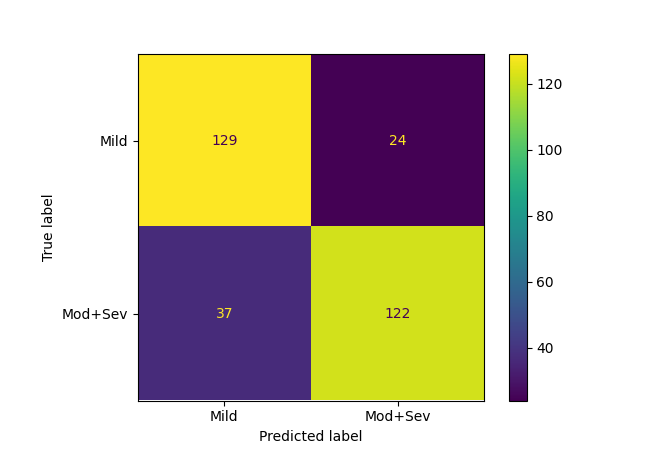
\includegraphics[width=1.05\linewidth,height=0.6\textheight]{figure/rf_bin_conf} 

}

\caption{İki Sınıflı Rassal Ormanlar Modeli Karmaşıklık Matrisi}\label{fig:unnamed-chunk-67}
\end{figure}
\begin{figure}

{\centering 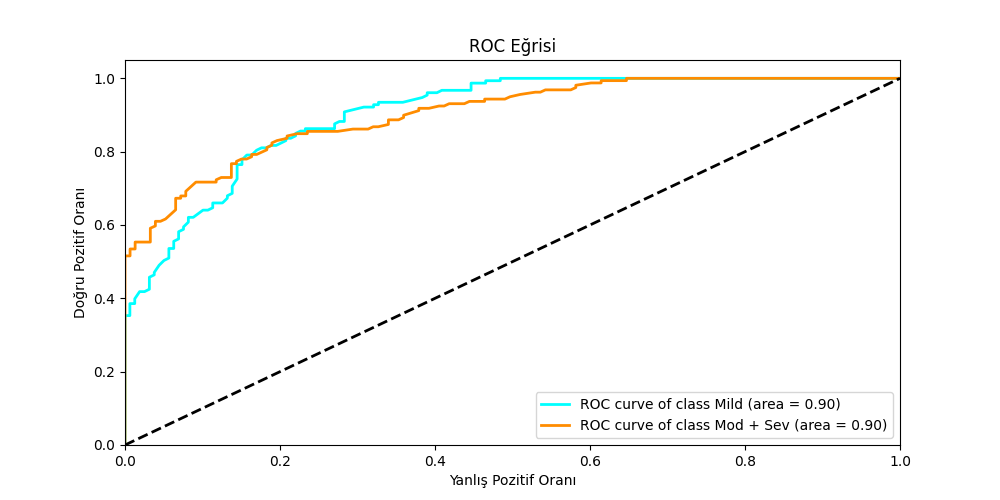
\includegraphics[width=1.05\linewidth,height=0.6\textheight]{figure/RandomForestClassifier_binary_roc} 

}

\caption{İki Sınıflı Rassal Ormanlar Modeli ROC Eğrisi ve AUC Değerleri}\label{fig:unnamed-chunk-68}
\end{figure}
\hypertarget{bin_xgb}{%
\subsection{XGBoost}\label{bin_xgb}}

Bu bölümde veri seti üzerinde xgboost modeli kullanılmış ve çıktıları değerlendirilmiştir.

\hypertarget{hiper-parametre-seuxe7imi-6}{%
\subsubsection{Hiper Parametre Seçimi}\label{hiper-parametre-seuxe7imi-6}}

Daha önce belirlenen parametre uzayını ve Scikit-Learn kütüphanesinde bulunan GridSearchCV algoritması ile en yüksek doğruluk oranı yakalanana kadar çalışması sağlanmıştır.
\begin{figure}

{\centering 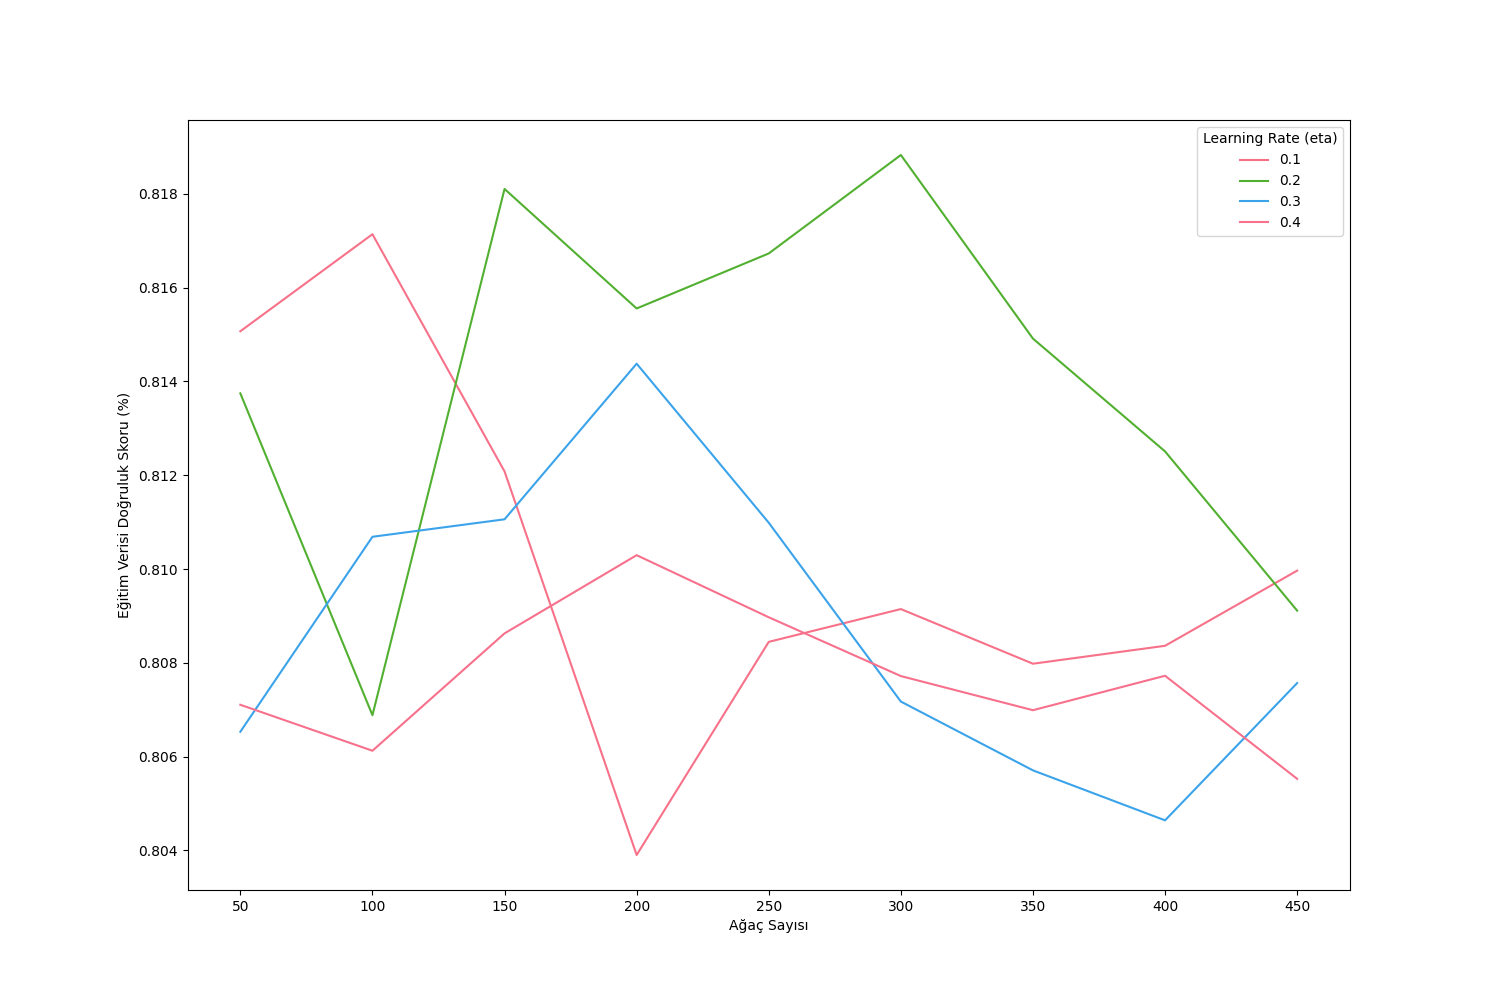
\includegraphics[width=1.1\linewidth,height=0.55\textheight]{figure/XGB_bin_Grid_Graph} 

}

\caption{İki Sınıflı XGBoost Modeli Eğitim Verisi Doğruluk Skorları}\label{fig:unnamed-chunk-70}
\end{figure}
XGBoost modeli için en yüksek doğruluk oranı aşağıdaki parametreler ile bulunmuştur;
\begin{itemize}
\tightlist
\item
  `eta': 0.2\\
\item
  `max\_depth': 10\\
\item
  `min\_child\_weight': 10\\
\item
  `n\_estimators': 400\\
  \newpage  
\end{itemize}
\hypertarget{en-iyi-parametreli-model-4}{%
\subsubsection{En İyi Parametreli Model}\label{en-iyi-parametreli-model-4}}

Bulunan parametrelerle kurulan modelin sınıflandırma metrikleri aşağıdaki gibidir.
\begin{verbatim}
              precision    recall  f1-score   support

        Mild       0.82      0.82      0.82       153
     Mod+Sev       0.82      0.83      0.83       159

    accuracy                           0.82       312
   macro avg       0.82      0.82      0.82       312
weighted avg       0.82      0.82      0.82       312
\end{verbatim}
\begin{verbatim}
Balanced Accuracy Score : 0.8235910716487853
\end{verbatim}
\begin{figure}

{\centering 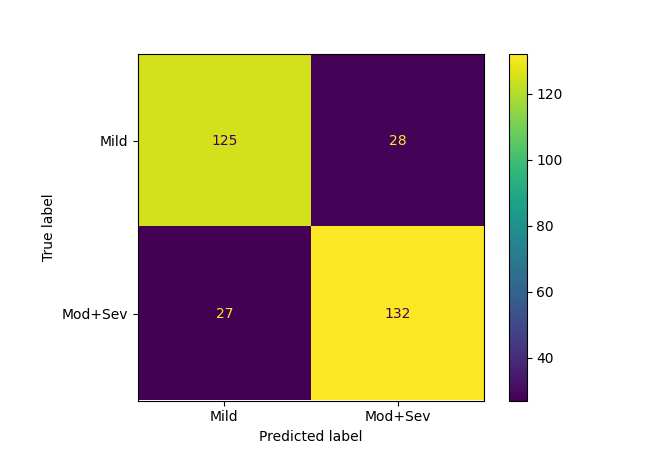
\includegraphics[width=1.05\linewidth,height=0.6\textheight]{figure/XGB_bin_conf} 

}

\caption{İki Sınıflı XGBoost Modeli Karmaşıklık Matrisi}\label{fig:unnamed-chunk-75}
\end{figure}
\begin{figure}

{\centering 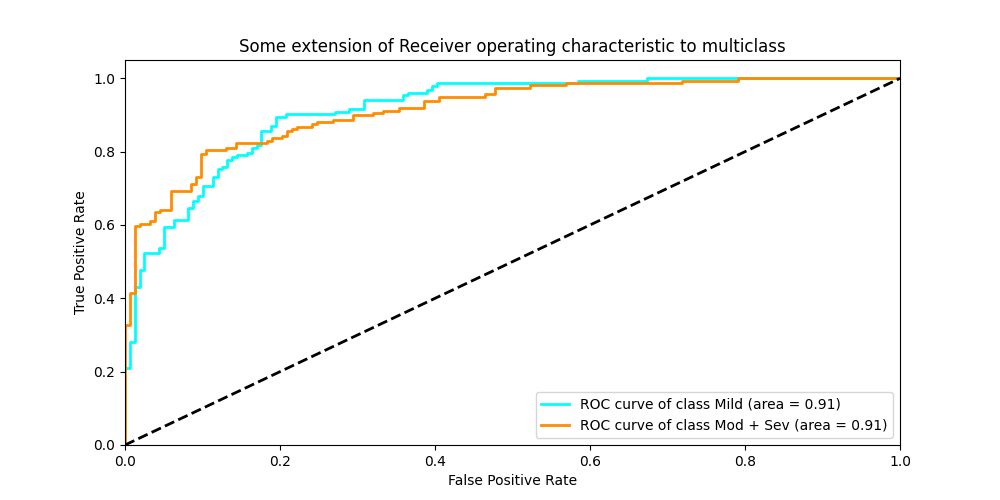
\includegraphics[width=1.05\linewidth,height=0.6\textheight]{figure/XGBClassifier_binary_roc} 

}

\caption{İki Sınıflı XGBoost Modeli ROC Eğrisi ve AUC Değerleri}\label{fig:unnamed-chunk-76}
\end{figure}
\hypertarget{bin_nn}{%
\subsection{Neural Network (Yapay Sinir Ağları) Modeli}\label{bin_nn}}

Bu bölümde veri seti üzerinde yapay sinir ağları modeli kullanılmış ve çıktıları değerlendirilmiştir.

\hypertarget{hiper-parametre-seuxe7imi-7}{%
\subsubsection{Hiper Parametre Seçimi}\label{hiper-parametre-seuxe7imi-7}}

Daha önce belirlenen parametre uzayını ve Scikit-Learn kütüphanesinde bulunan GridSearchCV algoritması ile en yüksek doğruluk oranı yakalanana kadar çalışması sağlanmıştır.
\begin{figure}

{\centering 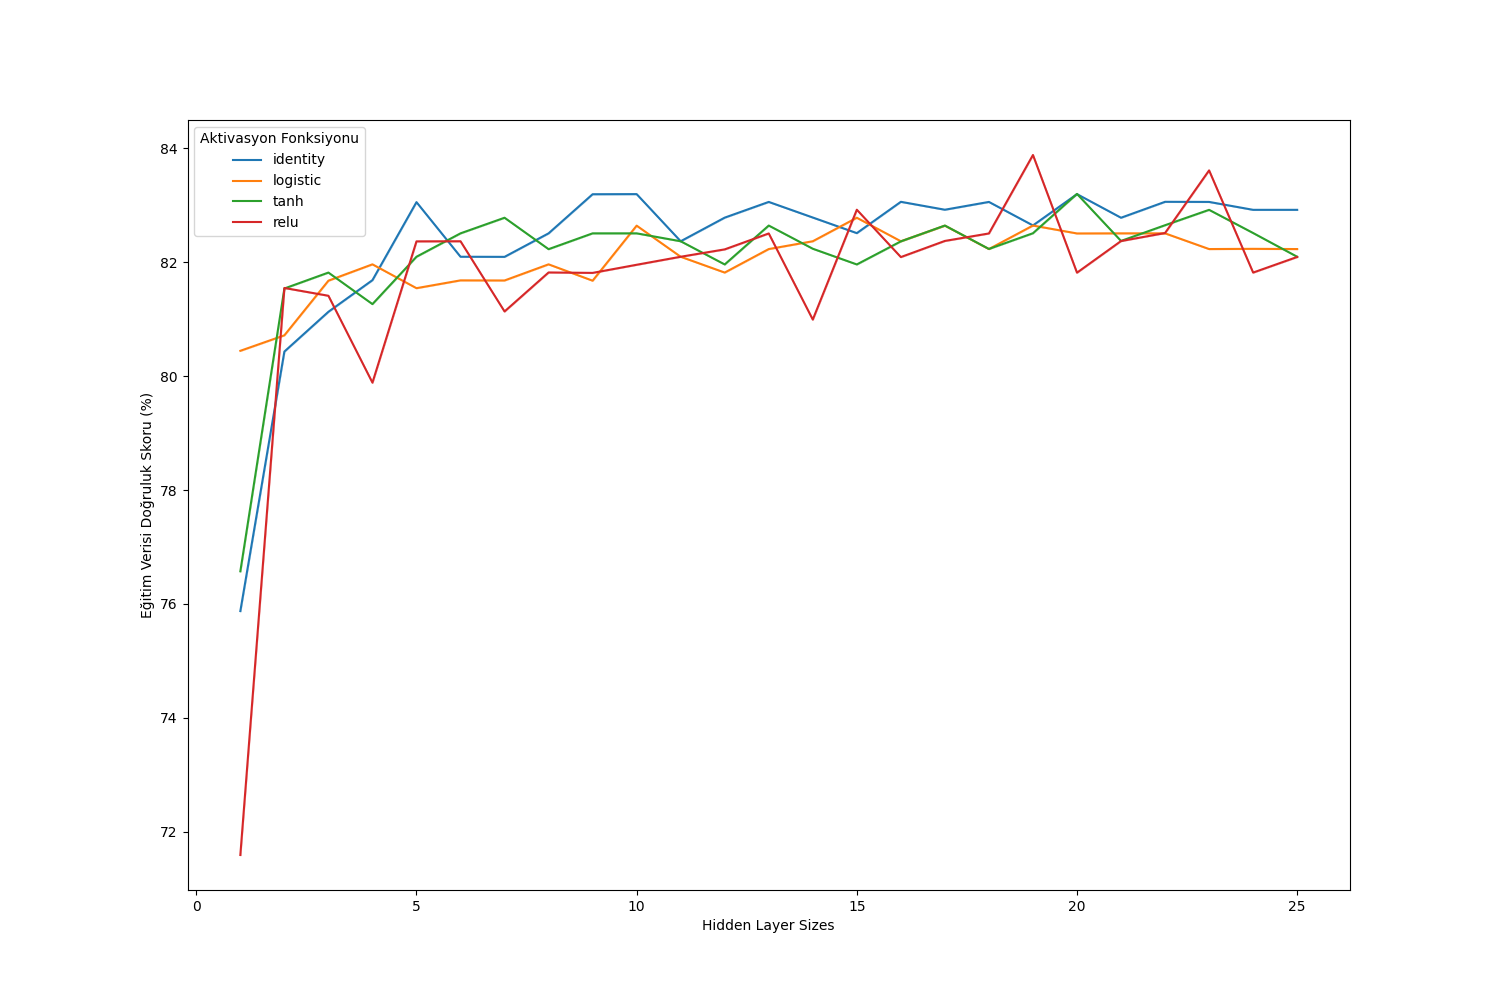
\includegraphics[width=1.1\linewidth,height=0.55\textheight]{figure/NN_bin_Grid_Graph} 

}

\caption{İki Sınıflı Yapay Sinir Ağları Modeli Eğitim Verisi Doğruluk Skorları}\label{fig:unnamed-chunk-78}
\end{figure}
Yapay sinir ağları modeli için en yüksek doğruluk oranı aşağıdaki parametreler ile bulunmuştur;
\begin{itemize}
\tightlist
\item
  `activation': `relu'\\
\item
  `hidden\_layer\_sizes': 19\\
\item
  `learning\_rate': `adaptive'\\
  \newpage  
\end{itemize}
\hypertarget{en-iyi-parametreli-model-5}{%
\subsubsection{En İyi Parametreli Model}\label{en-iyi-parametreli-model-5}}

Bulunan parametrelerle kurulan modelin sınıflandırma metrikleri aşağıdaki gibidir.
\begin{verbatim}
              precision    recall  f1-score   support

        Mild       0.78      0.85      0.82       153
     Mod+Sev       0.84      0.77      0.81       159

    accuracy                           0.81       312
   macro avg       0.81      0.81      0.81       312
weighted avg       0.81      0.81      0.81       312
\end{verbatim}
\begin{verbatim}
Balanced Accuracy Score : 0.8116290541373783
\end{verbatim}
\begin{figure}

{\centering 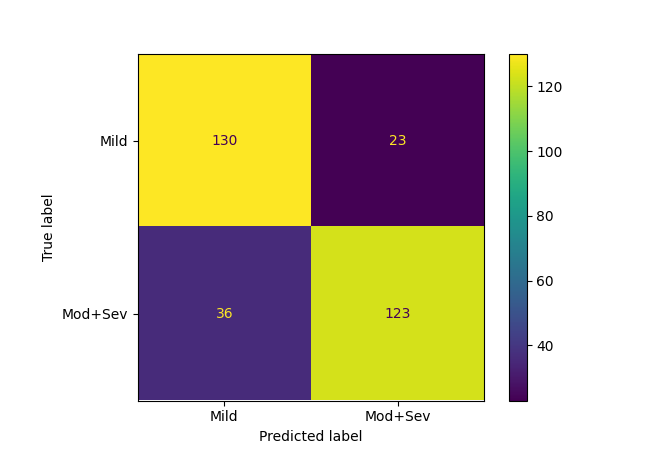
\includegraphics[width=1.05\linewidth,height=0.6\textheight]{figure/nn_bin_conf} 

}

\caption{İki Sınıflı Yapay Sinir Ağları Modeli Karmaşıklık Matrisi}\label{fig:unnamed-chunk-83}
\end{figure}
\begin{figure}

{\centering 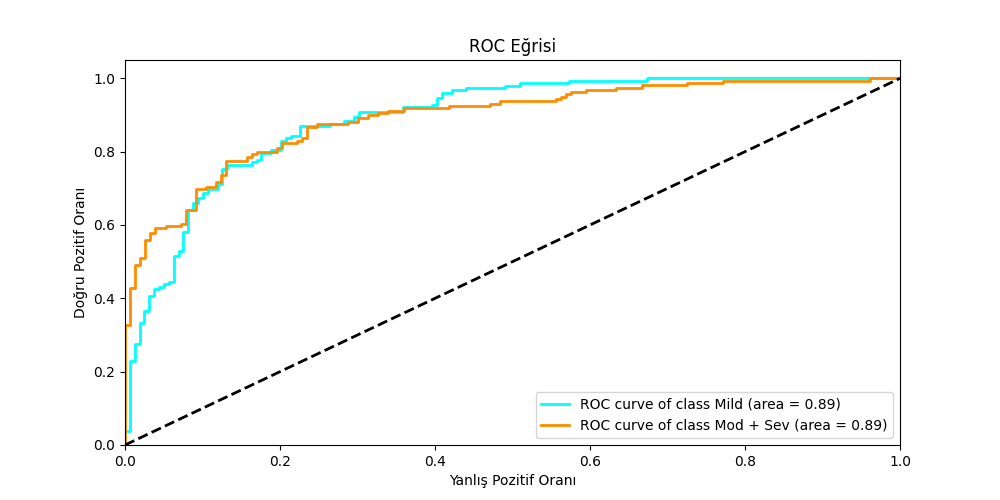
\includegraphics[width=1.05\linewidth,height=0.6\textheight]{figure/MLPClassifier_binary_roc} 

}

\caption{İki Sınıflı Yapay Sinir Ağları Modeli ROC Eğrisi ve AUC Değerleri}\label{fig:unnamed-chunk-84}
\end{figure}
\hypertarget{iki-sux131nux131flux131-sux131nux131flama-probleminin-modellerinin-deux11ferlendirdirilmesi}{%
\subsection{İki Sınıflı Sınıflama Probleminin Modellerinin Değerlendirdirilmesi}\label{iki-sux131nux131flux131-sux131nux131flama-probleminin-modellerinin-deux11ferlendirdirilmesi}}

Bölüm \ref{bin_knn}, \ref{bin_rf}, \ref{bin_xgb} ve \ref{bin_nn}`den elde edilen sonuçlar incelenmiş olup, iki sınıflı problem için \%82 doğru sınıflama oranları ile XGBoost ve Rassal Ormanlar modelleri en iyi modeller olarak bulunmuştur.\\
Bölüm \ref{bin_rf} ve \ref{bin_xgb}'de bulunan performans metrikleri yakından incelendiğinde, XGBoost modeli kesinlik, duyarlılık ve f1-skor metrikleri bakımından Rassal Ormanlar modelinden daha iyi sonuç vermiştir.\\
Ciddiyet sınıflandırma probleminin 'Mild' ve `Moderate + Severe' olacak şekilde 2 sınıfa indirgendiği durumda XGBoost modeli diğer modellerden daha iyi sonuç vermektedir.

\hypertarget{sonuuxe7}{%
\chapter*{Sonuç}\label{sonuuxe7}}
\addcontentsline{toc}{chapter}{Sonuç}

If we don't want Conclusion to have a chapter number next to it, we can add the \texttt{\{-\}} attribute.

\textbf{More info}

And here's some other random info: the first paragraph after a chapter title or section head \emph{shouldn't be} indented, because indents are to tell the reader that you're starting a new paragraph. Since that's obvious after a chapter or section title, proper typesetting doesn't add an indent there.

\hypertarget{kaynaklar}{%
\chapter*{Kaynaklar}\label{kaynaklar}}
\addcontentsline{toc}{chapter}{Kaynaklar}

\markboth{Kaynaklar}{Kaynaklar}

\hypertarget{refs}{}
\begin{CSLReferences}{1}{0}
\leavevmode\vadjust pre{\hypertarget{ref-ardakani2020diagnosis}{}}%
Ardakani, A. A., Afshar, A., Bhatt, S., Bureau, N. J., Tahmasebi, A., Acharya, U. R. ve Mohammadi, A. (2020). Diagnosis of carpal tunnel syndrome: A comparative study of shear wave elastography, morphometry and artificial intelligence techniques. \emph{Pattern Recognition Letters}, \emph{133}, 77-85.

\leavevmode\vadjust pre{\hypertarget{ref-aroori77carpal}{}}%
Aroori, S. ve Spence, R. (2008). Carpal Tunnel Syndrome. \emph{The Ulster Medical Society}, \emph{77}, 1-17.

\leavevmode\vadjust pre{\hypertarget{ref-avi2022}{}}%
Arora, A. (2022, Mart). 8 unique machine learning interview questions on backpropagation. \emph{Analytics Arora}. \url{https://analyticsarora.com/8-unique-machine-learning-interview-questions-on-backpropagation/} adresinden erişildi.

\leavevmode\vadjust pre{\hypertarget{ref-kts_bagatur}{}}%
Bagatur, A. E. (2006). Karpal Tünel Sendromu. \emph{Türkiye Klinikleri J Surg Med Sci.}, \emph{2}(17), 52-63.

\leavevmode\vadjust pre{\hypertarget{ref-breiman1997arcing}{}}%
Breiman, Leo. (1997). \emph{Arcing the edge}. Technical Report 486, Statistics Department, University of California.

\leavevmode\vadjust pre{\hypertarget{ref-breiman1991}{}}%
Breiman, Leo. (1999). 1 RANDOM FORESTS--RANDOM FEATURES.

\leavevmode\vadjust pre{\hypertarget{ref-breimanclassification}{}}%
Breiman, L., Friedman, J., Olshen, R. ve Stone, C. (t.y.). \emph{Classification and Regression Trees. 1984 Monterey, CA Wadsworth \& Brooks}. \emph{Cole Advanced Books \& Software Google Scholar}.

\leavevmode\vadjust pre{\hypertarget{ref-chen2016xgboost}{}}%
Chen, T. ve Guestrin, C. (2016). Xgboost: A scalable tree boosting system. \emph{Proceedings of the 22nd acm sigkdd international conference on knowledge discovery and data mining} içinde (ss. 785-794).

\leavevmode\vadjust pre{\hypertarget{ref-knn-info}{}}%
Cover, T. ve Hart, P. (1967). Nearest neighbor pattern classification. \emph{IEEE Transactions on Information Theory}, \emph{13}(1), 21-27. doi:\href{https://doi.org/10.1109/TIT.1967.1053964}{10.1109/TIT.1967.1053964}

\leavevmode\vadjust pre{\hypertarget{ref-dikker2017master}{}}%
Dikker, J. (2017). Master thesis Boosted tree learning for balanced item recommendation in online retail.

\leavevmode\vadjust pre{\hypertarget{ref-doad2013review}{}}%
Doad, P. ve Bartere, M. (2013). A Review: Study of Various Clustering Techniques. \emph{International Journal of Engineering Research \& Technology}, \emph{2}(11), 3141-3145.

\leavevmode\vadjust pre{\hypertarget{ref-greedy}{}}%
Friedman, J. H. (2001). Greedy function approximation: A gradient boosting machine. \emph{The Annals of Statistics}, \emph{29}(5).

\leavevmode\vadjust pre{\hypertarget{ref-ghasemi2014handy}{}}%
Ghasemi-Rad, M., Nosair, E., Vegh, A., Mohammadi, A., Akkad, A., Lesha, E., \ldots{} others. (2014). A handy review of carpal tunnel syndrome: From anatomy to diagnosis and treatment. \emph{World journal of radiology}, \emph{6}(6), 284.

\leavevmode\vadjust pre{\hypertarget{ref-hastie_tibshirani_friedman_2009}{}}%
Hastie, T., Tibshirani, R. ve Friedman, J. (2009). \emph{The elements of Statistical Learning, second edition: Data Mining, Inference, and prediction}. Springer.

\leavevmode\vadjust pre{\hypertarget{ref-koyama2021screening}{}}%
Koyama, T., Sato, S., Toriumi, M., Watanabe, T., Nimura, A., Okawa, A., \ldots{} Fujita, K. (2021). A Screening Method Using Anomaly Detection on a Smartphone for Patients With Carpal Tunnel Syndrome: Diagnostic Case-Control Study. \emph{JMIR mHealth and uHealth}, \emph{9}(3), e26320.

\leavevmode\vadjust pre{\hypertarget{ref-kumacs2005idiyopatik}{}}%
Kumaş, F. F. (2005).{I}diyopatik karpal t{"u}nel sendromu tedavisinde terap{"o}tik ultrason, steroid enjeksiyonu ve splint kullan{ı}m{ı}n{ı}n etkinli{ğ}inin randimize kontroll{"u} ara{ş}t{ı}r{ı}lmas{ı}.

\leavevmode\vadjust pre{\hypertarget{ref-kurt2020karpal}{}}%
Kurt, A. (2020). \emph{Karpal t{"u}nel sendrom hastalar{ı}nda bilateral ince motor beceri, skapular diskinezi, hareket korkusu ve fonksiyonun sa{ğ}l{ı}kl{ı}larla kar{ş}{ı}la{ş}t{ı}r{ı}lmas{ı}}. (Yayımlanmamış mathesis). Sa{ğ}l{ı}k Bilimleri Enstit{"u}s{"u}.

\leavevmode\vadjust pre{\hypertarget{ref-levine1993self}{}}%
Levine, D. W., Simmons, B. P., Koris, M. J., Daltroy, L. H., Hohl, G. G., Fossel, A. H. ve Katz, J. N. (1993). A self-administered questionnaire for the assessment of severity of symptoms and functional status in carpal tunnel syndrome. \emph{The Journal of bone and joint surgery. American volume}, \emph{75}(11), 1585-1592.

\leavevmode\vadjust pre{\hypertarget{ref-1995love}{}}%
Love, J. (1955). Median neuritis or carpal tunnel syndrome; diagnosis and treatment. \emph{North Carolina medical journal}, \emph{16}(10), 463-469.

\leavevmode\vadjust pre{\hypertarget{ref-mason1999boosting}{}}%
Mason, L., Baxter, J., Bartlett, P. ve Frean, M. (1999). Boosting algorithms as gradient descent. \emph{Advances in neural information processing systems}, \emph{12}.

\leavevmode\vadjust pre{\hypertarget{ref-mining2006data}{}}%
Mining, W. I. D. (2006). Data mining: Concepts and techniques. \emph{Morgan Kaufinann}, \emph{10}, 559-569.

\leavevmode\vadjust pre{\hypertarget{ref-mlmcgraw}{}}%
Mitchell, T. M. ve Learning, M. (1997). McGraw-Hill. \emph{New York}, 154-200.

\leavevmode\vadjust pre{\hypertarget{ref-oztemel2003yapay}{}}%
Öztemel, E. (2003). Yapay sinir ağlari. \emph{PapatyaYayincilik, Istanbul}.

\leavevmode\vadjust pre{\hypertarget{ref-park2021machine}{}}%
Park, D., Kim, B. H., Lee, S.-E., Kim, D. Y., Kim, M., Kwon, H. D., \ldots{} Lee, J. W. (2021). Machine learning-based approach for disease severity classification of carpal tunnel syndrome. \emph{Scientific Reports}, \emph{11}(1), 1-10.

\leavevmode\vadjust pre{\hypertarget{ref-history1988}{}}%
Pfeffer, G., Gelberman, R., Boyes, J. ve Rydevik, B. (1988). The history of carpal tunnnel syndrome. \emph{The Journal of Hand Surgery: British \& European Volume}, \emph{13}(1), 28-34.

\leavevmode\vadjust pre{\hypertarget{ref-quinlan2014c4}{}}%
Quinlan, J. R. (2014). \emph{C4. 5: programs for machine learning}. Elsevier.

\leavevmode\vadjust pre{\hypertarget{ref-robbins1963anatomical}{}}%
Robbins, H. (1963). Anatomical study of the median nerve in the carpal tunnel and etiologies of the carpal-tunnel syndrome. \emph{JBJS}, \emph{45}(5), 953-966.

\leavevmode\vadjust pre{\hypertarget{ref-sahu_2021}{}}%
Sahu, V. (2021, Haziran). Power of a single neuron. \emph{Medium}. Towards Data Science. \url{https://towardsdatascience.com/power-of-a-single-neuron-perceptron-c418ba445095} adresinden erişildi.

\leavevmode\vadjust pre{\hypertarget{ref-salam2018evaluating}{}}%
Salam Patrous, Z. (2018). Evaluating XGBoost for user classification by using behavioral features extracted from smartphone sensors.

\leavevmode\vadjust pre{\hypertarget{ref-sezgi2006assessment}{}}%
Sezgin, M., İncel, N. A., Sevim, S., Çamdeviren, H., As, İ. ve Erdoğan, C. (2006). Assessment of symptom severity and functional status in patients with carpal tunnel syndrome: reliability and validity of the Turkish version of the Boston Questionnaire. \emph{Disability and rehabilitation}, \emph{28}(20), 1281-1286.

\leavevmode\vadjust pre{\hypertarget{ref-tibco}{}}%
TIBCO. (t.y.). What is a random forest? \emph{TIBCO Software}. \url{https://www.tibco.com/reference-center/what-is-a-random-forest} adresinden erişildi.

\leavevmode\vadjust pre{\hypertarget{ref-werner2002carpal}{}}%
Werner, R. A. ve Andary, M. (2002). Carpal tunnel syndrome: pathophysiology and clinical neurophysiology. \emph{Clinical Neurophysiology}, \emph{113}(9), 1373-1381.

\leavevmode\vadjust pre{\hypertarget{ref-yangin2019xgboost}{}}%
Yangın, G. (2019). \emph{Xgboost ve karar ağaçları tabanlı algoritmaların diyabet veri setleri üzerine uygulaması}. (Yayımlanmamış doktora tezi). Yüksek Lisans Tezi, Mimar Sinan Güzel Sanatlar Üniversitesi Fen Bilimleri.

\end{CSLReferences}
\setlength{\parindent}{-0.20in}
\setlength{\leftskip}{0.20in}
\setlength{\parskip}{8pt}

\appendix

\hypertarget{gerekli-paketlerin-yuxfcklenmesi-ve-verilerin-okunmasux131-ve-veri-uxf6niux15fleme}{%
\chapter{Gerekli Paketlerin Yüklenmesi ve Verilerin Okunması ve Veri Önişleme}\label{gerekli-paketlerin-yuxfcklenmesi-ve-verilerin-okunmasux131-ve-veri-uxf6niux15fleme}}

\scriptsize
\begin{Shaded}
\begin{Highlighting}[]
\CommentTok{\# R için gerekli paketlerin kurulması}
\ControlFlowTok{if}\NormalTok{(}\SpecialCharTok{!}\FunctionTok{require}\NormalTok{(reticulate)) }\FunctionTok{install.packages}\NormalTok{(}\StringTok{"reticulate"}\NormalTok{, }\AttributeTok{repos =} \StringTok{"http://cran.rstudio.com"}\NormalTok{)}
\ControlFlowTok{if}\NormalTok{(}\SpecialCharTok{!}\FunctionTok{require}\NormalTok{(tidyverse)) }\FunctionTok{install.packages}\NormalTok{(}\StringTok{"tidyverse"}\NormalTok{, }\AttributeTok{repos =} \StringTok{"http://cran.rstudio.com"}\NormalTok{)}
\ControlFlowTok{if}\NormalTok{(}\SpecialCharTok{!}\FunctionTok{require}\NormalTok{(caret)) }\FunctionTok{install.packages}\NormalTok{(}\StringTok{"caret"}\NormalTok{,}\AttributeTok{repos =} \StringTok{"http://cran.rstudio.com"}\NormalTok{)}
\ControlFlowTok{if}\NormalTok{(}\SpecialCharTok{!}\FunctionTok{require}\NormalTok{(caretEnsemble))  }\FunctionTok{install.packages}\NormalTok{(}\StringTok{"caretEnsemble"}\NormalTok{,}\AttributeTok{repos =} \StringTok{"http://cran.rstudio.com"}\NormalTok{)}
\ControlFlowTok{if}\NormalTok{(}\SpecialCharTok{!}\FunctionTok{require}\NormalTok{(doParallel))  }\FunctionTok{install.packages}\NormalTok{(}\StringTok{"doParallel"}\NormalTok{,}\AttributeTok{repos =} \StringTok{"http://cran.rstudio.com"}\NormalTok{)}
\ControlFlowTok{if}\NormalTok{(}\SpecialCharTok{!}\FunctionTok{require}\NormalTok{(data.table))  }\FunctionTok{install.packages}\NormalTok{(}\StringTok{"data.table"}\NormalTok{,}\AttributeTok{repos =} \StringTok{"http://cran.rstudio.com"}\NormalTok{)}
\ControlFlowTok{if}\NormalTok{(}\SpecialCharTok{!}\FunctionTok{require}\NormalTok{(dplyr))  }\FunctionTok{install.packages}\NormalTok{(}\StringTok{"dplyr"}\NormalTok{,}\AttributeTok{repos =} \StringTok{"http://cran.rstudio.com"}\NormalTok{)}
\ControlFlowTok{if}\NormalTok{(}\SpecialCharTok{!}\FunctionTok{require}\NormalTok{(e1071))  }\FunctionTok{install.packages}\NormalTok{(}\StringTok{"e1071"}\NormalTok{,}\AttributeTok{repos =} \StringTok{"http://cran.rstudio.com"}\NormalTok{)}
\CommentTok{\#if(!require(gbm))  install.packages("gbm",repos = "http://cran.rstudio.com")}
\ControlFlowTok{if}\NormalTok{(}\SpecialCharTok{!}\FunctionTok{require}\NormalTok{(kernlab))  }\FunctionTok{install.packages}\NormalTok{(}\StringTok{"kernlab"}\NormalTok{,}\AttributeTok{repos =} \StringTok{"http://cran.rstudio.com"}\NormalTok{)}
\CommentTok{\#if(!require(randomForest))  install.packages("randomForest",repos = "http://cran.rstudio.com")}
\ControlFlowTok{if}\NormalTok{(}\SpecialCharTok{!}\FunctionTok{require}\NormalTok{(tidyverse))  }\FunctionTok{install.packages}\NormalTok{(}\StringTok{"tidyverse"}\NormalTok{,}\AttributeTok{repos =} \StringTok{"http://cran.rstudio.com"}\NormalTok{)}
\CommentTok{\#if(!require(xgboost))  install.packages("xgboost",repos = "http://cran.rstudio.com")}
\ControlFlowTok{if}\NormalTok{(}\SpecialCharTok{!}\FunctionTok{require}\NormalTok{(smotefamily))  }\FunctionTok{install.packages}\NormalTok{(}\StringTok{"smotefamily"}\NormalTok{,}\AttributeTok{repos =} \StringTok{"http://cran.rstudio.com"}\NormalTok{)}
\end{Highlighting}
\end{Shaded}
\begin{Shaded}
\begin{Highlighting}[]
\CommentTok{\# Python için gerekli paketlerin ve veri setinin yüklenmesi}
\ImportTok{import}\NormalTok{ warnings}
\NormalTok{warnings.filterwarnings(}\StringTok{"ignore"}\NormalTok{, category}\OperatorTok{=}\PreprocessorTok{FutureWarning}\NormalTok{)}
\ImportTok{from}\NormalTok{ warnings }\ImportTok{import}\NormalTok{ simplefilter}
\NormalTok{simplefilter(action}\OperatorTok{=}\StringTok{\textquotesingle{}ignore\textquotesingle{}}\NormalTok{, category}\OperatorTok{=}\PreprocessorTok{FutureWarning}\NormalTok{)}
\ImportTok{import}\NormalTok{ numpy }\ImportTok{as}\NormalTok{ np, pandas }\ImportTok{as}\NormalTok{ pd, matplotlib.pyplot }\ImportTok{as}\NormalTok{ plt}
\ImportTok{import}\NormalTok{ seaborn }\ImportTok{as}\NormalTok{ sns}
\ImportTok{from}\NormalTok{ sklearn.feature\_selection }\ImportTok{import}\NormalTok{ VarianceThreshold}
\ImportTok{from}\NormalTok{ scipy.stats }\ImportTok{import}\NormalTok{ f\_oneway, chi2\_contingency}
\NormalTok{CTS }\OperatorTok{=}\NormalTok{ pd.read\_csv(}\StringTok{"data/CTS.csv"}\NormalTok{,sep}\OperatorTok{=}\StringTok{","}\NormalTok{)}
\NormalTok{dataGroup }\OperatorTok{=}\NormalTok{ CTS[[}\StringTok{"Severity"}\NormalTok{,}\StringTok{"Age"}\NormalTok{,}\StringTok{"BMI"}\NormalTok{,}\StringTok{"CSA"}\NormalTok{,}\StringTok{"PB"}\NormalTok{,}\StringTok{"Duration"}\NormalTok{,}\StringTok{"NRS"}\NormalTok{]]}
\NormalTok{dataOverall }\OperatorTok{=}\NormalTok{ CTS[[}\StringTok{"Age"}\NormalTok{,}\StringTok{"BMI"}\NormalTok{,}\StringTok{"CSA"}\NormalTok{,}\StringTok{"PB"}\NormalTok{,}\StringTok{"Duration"}\NormalTok{,}\StringTok{"NRS"}\NormalTok{]]}
\NormalTok{meanoval, stdoval }\OperatorTok{=} \BuiltInTok{round}\NormalTok{(dataOverall.mean(),}\DecValTok{1}\NormalTok{), }\BuiltInTok{round}\NormalTok{(dataOverall.std(ddof}\OperatorTok{=}\DecValTok{1}\NormalTok{),}\DecValTok{1}\NormalTok{)}
\NormalTok{means }\OperatorTok{=} \BuiltInTok{round}\NormalTok{(dataGroup.groupby(}\StringTok{"Severity"}\NormalTok{).mean(),}\DecValTok{1}\NormalTok{)}
\NormalTok{stds }\OperatorTok{=} \BuiltInTok{round}\NormalTok{(dataGroup.groupby(}\StringTok{"Severity"}\NormalTok{).std(ddof}\OperatorTok{=}\DecValTok{1}\NormalTok{),}\DecValTok{1}\NormalTok{)}
\CommentTok{\#\#}
\NormalTok{mild }\OperatorTok{=}\NormalTok{ CTS[CTS.Severity }\OperatorTok{==} \StringTok{"mild"}\NormalTok{]}
\NormalTok{moderate }\OperatorTok{=}\NormalTok{ CTS[CTS.Severity }\OperatorTok{==} \StringTok{"moderate"}\NormalTok{]}
\NormalTok{severe }\OperatorTok{=}\NormalTok{ CTS[CTS.Severity }\OperatorTok{==} \StringTok{"severe"}\NormalTok{]}
\NormalTok{numVar }\OperatorTok{=}\NormalTok{ [}\StringTok{"Age"}\NormalTok{,}\StringTok{"BMI"}\NormalTok{,}\StringTok{"CSA"}\NormalTok{,}\StringTok{"PB"}\NormalTok{,}\StringTok{"Duration"}\NormalTok{,}\StringTok{"NRS"}\NormalTok{]}
\NormalTok{catVar }\OperatorTok{=}\NormalTok{ [}\StringTok{"Sex"}\NormalTok{,}\StringTok{"Side"}\NormalTok{,}\StringTok{"Diabetes"}\NormalTok{,}\StringTok{"NP"}\NormalTok{,}\StringTok{"Weakness"}\NormalTok{]}
\NormalTok{p\_values }\OperatorTok{=}\NormalTok{ []}
\NormalTok{p\_vals2 }\OperatorTok{=}\NormalTok{ []}
\ControlFlowTok{for}\NormalTok{ i }\KeywordTok{in}\NormalTok{ numVar:}
\NormalTok{    \_,p\_val }\OperatorTok{=}\NormalTok{ f\_oneway(mild[i],moderate[i],severe[i])}
\NormalTok{    p\_values.append(}\BuiltInTok{round}\NormalTok{(p\_val,}\DecValTok{3}\NormalTok{))}
\ControlFlowTok{for}\NormalTok{ i }\KeywordTok{in}\NormalTok{ catVar:}
\NormalTok{    var\_0 }\OperatorTok{=}\NormalTok{ np.array([}\BuiltInTok{sum}\NormalTok{(mild[i] }\OperatorTok{==} \DecValTok{0}\NormalTok{),}\BuiltInTok{sum}\NormalTok{(moderate[i] }\OperatorTok{==} \DecValTok{0}\NormalTok{),}\BuiltInTok{sum}\NormalTok{(severe[i] }\OperatorTok{==} \DecValTok{0}\NormalTok{)])}
\NormalTok{    var\_1 }\OperatorTok{=}\NormalTok{ np.array([}\BuiltInTok{sum}\NormalTok{(mild[i] }\OperatorTok{==} \DecValTok{1}\NormalTok{),}\BuiltInTok{sum}\NormalTok{(moderate[i] }\OperatorTok{==} \DecValTok{1}\NormalTok{),}\BuiltInTok{sum}\NormalTok{(severe[i] }\OperatorTok{==} \DecValTok{1}\NormalTok{)])}
\NormalTok{    p\_vals2.append(}\BuiltInTok{round}\NormalTok{(chi2\_contingency(np.array([var\_1,var\_0]),correction}\OperatorTok{=}\VariableTok{False}\NormalTok{)[}\DecValTok{1}\NormalTok{],}\DecValTok{3}\NormalTok{))}
\NormalTok{CTS\_kor }\OperatorTok{=}\NormalTok{ CTS.drop([}\StringTok{"Severity"}\NormalTok{,}\StringTok{"Mild"}\NormalTok{,}\StringTok{"Mod"}\NormalTok{,}\StringTok{"Sev"}\NormalTok{],axis}\OperatorTok{=}\DecValTok{1}\NormalTok{)}
\NormalTok{zeroVar }\OperatorTok{=}\NormalTok{ CTS\_kor.shape[}\DecValTok{1}\NormalTok{]}\OperatorTok{{-}}\NormalTok{((VarianceThreshold(threshold}\OperatorTok{=}\DecValTok{0}\NormalTok{).fit(CTS\_kor)).get\_support()).}\BuiltInTok{sum}\NormalTok{()    }
\CommentTok{\#\#\#\#\#\#}
\NormalTok{catDF }\OperatorTok{=}\NormalTok{ CTS.groupby(}\StringTok{"Severity"}\NormalTok{).}\BuiltInTok{sum}\NormalTok{()[[}\StringTok{"Sex"}\NormalTok{,}\StringTok{"Side"}\NormalTok{,}\StringTok{"Diabetes"}\NormalTok{,}\StringTok{"NP"}\NormalTok{,}\StringTok{"Weakness"}\NormalTok{]]}
\NormalTok{sex, rside, diab, np, weak }\OperatorTok{=}\NormalTok{ catDF[}\StringTok{"Sex"}\NormalTok{],catDF[}\StringTok{"Side"}\NormalTok{],catDF[}\StringTok{"Diabetes"}\NormalTok{],catDF[}\StringTok{"NP"}\NormalTok{],catDF[}\StringTok{"Weakness"}\NormalTok{]}
\NormalTok{hands }\OperatorTok{=}\NormalTok{ CTS.groupby(}\StringTok{"Severity"}\NormalTok{).count()[}\StringTok{"NP"}\NormalTok{]}
\NormalTok{handsx }\OperatorTok{=}\NormalTok{ hands}\OperatorTok{*}\DecValTok{100}
\end{Highlighting}
\end{Shaded}
\begin{Shaded}
\begin{Highlighting}[]
\CommentTok{\# R için veri setinin tanıtılması ve Rastgele olarak ayrılması}
\NormalTok{  means }\OtherTok{\textless{}{-}} \FunctionTok{as.data.frame}\NormalTok{(py}\SpecialCharTok{$}\NormalTok{means)}
\NormalTok{  stds }\OtherTok{\textless{}{-}} \FunctionTok{as.data.frame}\NormalTok{(py}\SpecialCharTok{$}\NormalTok{stds)}
\NormalTok{  meanOval }\OtherTok{\textless{}{-}} \FunctionTok{as.data.frame}\NormalTok{(}\FunctionTok{t}\NormalTok{(py}\SpecialCharTok{$}\NormalTok{meanoval))}
\NormalTok{  stdOval }\OtherTok{\textless{}{-}} \FunctionTok{as.data.frame}\NormalTok{(}\FunctionTok{t}\NormalTok{(py}\SpecialCharTok{$}\NormalTok{stdoval))}
\NormalTok{  CTS }\OtherTok{\textless{}{-}} \FunctionTok{as.data.frame}\NormalTok{(}\FunctionTok{read\_csv}\NormalTok{(}\StringTok{"data/CTS.csv"}\NormalTok{))}
\NormalTok{  seed}\OtherTok{\textless{}{-}}\DecValTok{0923}
  \FunctionTok{set.seed}\NormalTok{(seed)}
\NormalTok{  ind}\OtherTok{\textless{}{-}}\FunctionTok{sample}\NormalTok{(}\DecValTok{2}\NormalTok{,}\FunctionTok{nrow}\NormalTok{(CTS),}\AttributeTok{replace =}\NormalTok{ T,}\AttributeTok{prob =} \FunctionTok{c}\NormalTok{(}\FloatTok{0.7}\NormalTok{,}\FloatTok{0.3}\NormalTok{))}
\NormalTok{  traindata\_top }\OtherTok{\textless{}{-}}\NormalTok{ CTS[ind}\SpecialCharTok{==}\DecValTok{1}\NormalTok{,]}
\NormalTok{  testdata\_top }\OtherTok{\textless{}{-}}\NormalTok{ CTS[ind}\SpecialCharTok{==}\DecValTok{2}\NormalTok{,]}
\CommentTok{\# BURADAN SORNASI R VERİ ÖNİŞLEME}
\NormalTok{  CTS}\SpecialCharTok{$}\NormalTok{Severity}\OtherTok{\textless{}{-}}\FunctionTok{as.factor}\NormalTok{(CTS}\SpecialCharTok{$}\NormalTok{Severity)}
\NormalTok{  CTS}\SpecialCharTok{$}\NormalTok{Mild}\OtherTok{\textless{}{-}}\FunctionTok{as.factor}\NormalTok{(CTS}\SpecialCharTok{$}\NormalTok{Mild)}
\NormalTok{  CTS}\SpecialCharTok{$}\NormalTok{Mod}\OtherTok{\textless{}{-}}\FunctionTok{as.factor}\NormalTok{(CTS}\SpecialCharTok{$}\NormalTok{Mod)}
\NormalTok{  CTS}\SpecialCharTok{$}\NormalTok{Sev}\OtherTok{\textless{}{-}}\FunctionTok{as.factor}\NormalTok{(CTS}\SpecialCharTok{$}\NormalTok{Sev)}
\NormalTok{  CTS}\SpecialCharTok{$}\NormalTok{Sex }\OtherTok{\textless{}{-}}\FunctionTok{as.factor}\NormalTok{(CTS}\SpecialCharTok{$}\NormalTok{Sex)}
\NormalTok{  CTS}\SpecialCharTok{$}\NormalTok{Side }\OtherTok{\textless{}{-}}\FunctionTok{as.factor}\NormalTok{(CTS}\SpecialCharTok{$}\NormalTok{Side)}
\NormalTok{  CTS}\SpecialCharTok{$}\NormalTok{Diabetes }\OtherTok{\textless{}{-}}\FunctionTok{as.factor}\NormalTok{(CTS}\SpecialCharTok{$}\NormalTok{Diabetes)}
\NormalTok{  CTS}\SpecialCharTok{$}\NormalTok{NP }\OtherTok{\textless{}{-}} \FunctionTok{as.factor}\NormalTok{(CTS}\SpecialCharTok{$}\NormalTok{NP)}
\NormalTok{  CTS}\SpecialCharTok{$}\NormalTok{Weakness }\OtherTok{\textless{}{-}} \FunctionTok{as.factor}\NormalTok{(CTS}\SpecialCharTok{$}\NormalTok{Weakness)}
\NormalTok{  predata}\OtherTok{\textless{}{-}}\NormalTok{CTS}
\NormalTok{  st\_model}\OtherTok{\textless{}{-}}\FunctionTok{preProcess}\NormalTok{(predata[,}\DecValTok{5}\SpecialCharTok{:}\DecValTok{10}\NormalTok{], }\AttributeTok{method=}\FunctionTok{c}\NormalTok{(}\StringTok{"center"}\NormalTok{,}\StringTok{"scale"}\NormalTok{))}
\NormalTok{  data}\OtherTok{\textless{}{-}}\FunctionTok{predict}\NormalTok{(st\_model, predata)}
\NormalTok{  data}\OtherTok{=}\FunctionTok{as.data.frame}\NormalTok{(data)}
\NormalTok{  ohe\_feats }\OtherTok{=} \FunctionTok{c}\NormalTok{(}\StringTok{\textquotesingle{}Sex\textquotesingle{}}\NormalTok{,}\StringTok{\textquotesingle{}Side\textquotesingle{}}\NormalTok{,}\StringTok{\textquotesingle{}Diabetes\textquotesingle{}}\NormalTok{,}\StringTok{\textquotesingle{}NP\textquotesingle{}}\NormalTok{,}\StringTok{\textquotesingle{}Weakness\textquotesingle{}}\NormalTok{)}
\NormalTok{  dummies }\OtherTok{=} \FunctionTok{dummyVars}\NormalTok{(}\SpecialCharTok{\textasciitilde{}}\NormalTok{ Sex}\SpecialCharTok{+}\NormalTok{Side}\SpecialCharTok{+}\NormalTok{Diabetes}\SpecialCharTok{+}\NormalTok{NP}\SpecialCharTok{+}\NormalTok{Weakness, }\AttributeTok{data =}\NormalTok{ data)}
\NormalTok{  df\_ohe }\OtherTok{\textless{}{-}} \FunctionTok{as.data.frame}\NormalTok{(}\FunctionTok{predict}\NormalTok{(dummies, }\AttributeTok{newdata =}\NormalTok{ data))}
\NormalTok{  df\_combined }\OtherTok{\textless{}{-}} \FunctionTok{cbind}\NormalTok{(data[,}\SpecialCharTok{{-}}\FunctionTok{c}\NormalTok{(}\FunctionTok{which}\NormalTok{(}\FunctionTok{colnames}\NormalTok{(data) }\SpecialCharTok{\%in\%}\NormalTok{ ohe\_feats))],df\_ohe)}
\NormalTok{  dat }\OtherTok{=} \FunctionTok{as.data.table}\NormalTok{(df\_combined)}
\NormalTok{  traindata}\OtherTok{\textless{}{-}}\NormalTok{dat[ind}\SpecialCharTok{==}\DecValTok{1}\NormalTok{,]}
\NormalTok{  testdata}\OtherTok{\textless{}{-}}\NormalTok{dat[ind}\SpecialCharTok{==}\DecValTok{2}\NormalTok{,]}
\NormalTok{  trainmc}\OtherTok{\textless{}{-}}\NormalTok{traindata}
\NormalTok{  testmc}\OtherTok{\textless{}{-}}\NormalTok{testdata}
\NormalTok{  trainmc}\SpecialCharTok{$}\NormalTok{Mild}\OtherTok{=}\ConstantTok{NULL}
\NormalTok{  trainmc}\SpecialCharTok{$}\NormalTok{Mod}\OtherTok{=}\ConstantTok{NULL}
\NormalTok{  trainmc}\SpecialCharTok{$}\NormalTok{Sev}\OtherTok{=}\ConstantTok{NULL}
\NormalTok{  testmc}\SpecialCharTok{$}\NormalTok{Mild}\OtherTok{=}\ConstantTok{NULL}
\NormalTok{  testmc}\SpecialCharTok{$}\NormalTok{Mod}\OtherTok{=}\ConstantTok{NULL}
\NormalTok{  testmc}\SpecialCharTok{$}\NormalTok{Sev}\OtherTok{=}\ConstantTok{NULL}
\NormalTok{  hco }\OtherTok{\textless{}{-}} \FunctionTok{nrow}\NormalTok{(CTS)}
\NormalTok{  hco }\OtherTok{\textless{}{-}}\NormalTok{ hco }\SpecialCharTok{*} \DecValTok{100}
\end{Highlighting}
\end{Shaded}
\begin{Shaded}
\begin{Highlighting}[]
\CommentTok{\# Python için Veri Önişleme }
\ImportTok{from}\NormalTok{ sklearn.preprocessing }\ImportTok{import}\NormalTok{ LabelEncoder}
\ImportTok{from}\NormalTok{ sklearn.preprocessing }\ImportTok{import}\NormalTok{ StandardScaler}
\NormalTok{LE }\OperatorTok{=}\NormalTok{ LabelEncoder().fit([}\StringTok{"mild"}\NormalTok{,}\StringTok{"moderate"}\NormalTok{,}\StringTok{"severe"}\NormalTok{])}
\NormalTok{traindata\_P }\OperatorTok{=}\NormalTok{ pd.DataFrame(r.traindata\_top)}
\NormalTok{traindata\_P.drop([}\StringTok{"Mild"}\NormalTok{,}\StringTok{"Mod"}\NormalTok{,}\StringTok{"Sev"}\NormalTok{],axis}\OperatorTok{=}\DecValTok{1}\NormalTok{,inplace}\OperatorTok{=}\VariableTok{True}\NormalTok{)}
\NormalTok{testdata\_P }\OperatorTok{=}\NormalTok{ pd.DataFrame(r.testdata\_top)}
\NormalTok{testdata\_P.drop([}\StringTok{"Mild"}\NormalTok{,}\StringTok{"Mod"}\NormalTok{,}\StringTok{"Sev"}\NormalTok{],axis}\OperatorTok{=}\DecValTok{1}\NormalTok{,inplace}\OperatorTok{=}\VariableTok{True}\NormalTok{)}
\NormalTok{X\_train, X\_test, y\_train, y\_test }\OperatorTok{=}\NormalTok{ traindata\_P.drop([}\StringTok{"Severity"}\NormalTok{],axis}\OperatorTok{=}\DecValTok{1}\NormalTok{),testdata\_P.drop([}\StringTok{"Severity"}\NormalTok{],}
\NormalTok{axis}\OperatorTok{=}\DecValTok{1}\NormalTok{),pd.DataFrame(LE.transform(traindata\_P.Severity)),}
\NormalTok{pd.DataFrame(LE.transform(testdata\_P.Severity))}
\NormalTok{Stand }\OperatorTok{=}\NormalTok{ StandardScaler().fit(r.CTS[[}\StringTok{"Age"}\NormalTok{,}\StringTok{"BMI"}\NormalTok{,}\StringTok{"CSA"}\NormalTok{,}\StringTok{"PB"}\NormalTok{,}\StringTok{"Duration"}\NormalTok{,}\StringTok{"NRS"}\NormalTok{]])}
\NormalTok{X\_train[[}\StringTok{"Age"}\NormalTok{,}\StringTok{"BMI"}\NormalTok{,}\StringTok{"CSA"}\NormalTok{,}\StringTok{"PB"}\NormalTok{,}\StringTok{"Duration"}\NormalTok{,}\StringTok{"NRS"}\NormalTok{]]}\OperatorTok{=}\NormalTok{pd.DataFrame(Stand.transform(X\_train[[}\StringTok{"Age"}\NormalTok{,}\StringTok{"BMI"}\NormalTok{,}
\StringTok{"CSA"}\NormalTok{,}\StringTok{"PB"}\NormalTok{,}\StringTok{"Duration"}\NormalTok{,}\StringTok{"NRS"}\NormalTok{]]),columns}\OperatorTok{=}\NormalTok{[}\StringTok{"Age"}\NormalTok{,}\StringTok{"BMI"}\NormalTok{,}\StringTok{"CSA"}\NormalTok{,}\StringTok{"PB"}\NormalTok{,}\StringTok{"Duration"}\NormalTok{,}\StringTok{"NRS"}\NormalTok{])}
\NormalTok{y\_train }\OperatorTok{=}\NormalTok{ y\_train.to\_numpy().ravel()}
\NormalTok{X\_test[[}\StringTok{"Age"}\NormalTok{,}\StringTok{"BMI"}\NormalTok{,}\StringTok{"CSA"}\NormalTok{,}\StringTok{"PB"}\NormalTok{,}\StringTok{"Duration"}\NormalTok{,}\StringTok{"NRS"}\NormalTok{]] }\OperatorTok{=}\NormalTok{ pd.DataFrame(Stand.transform(X\_test[[}\StringTok{"Age"}\NormalTok{,}\StringTok{"BMI"}\NormalTok{,}
\StringTok{"CSA"}\NormalTok{,}\StringTok{"PB"}\NormalTok{,}\StringTok{"Duration"}\NormalTok{,}\StringTok{"NRS"}\NormalTok{]]),columns}\OperatorTok{=}\NormalTok{[}\StringTok{"Age"}\NormalTok{,}\StringTok{"BMI"}\NormalTok{,}\StringTok{"CSA"}\NormalTok{,}\StringTok{"PB"}\NormalTok{,}\StringTok{"Duration"}\NormalTok{,}\StringTok{"NRS"}\NormalTok{])}
\NormalTok{y\_test }\OperatorTok{=}\NormalTok{ y\_test.to\_numpy().ravel()}
\end{Highlighting}
\end{Shaded}
\normalsize

\hypertarget{sux131nux131flandux131rma-uxfcuxe7-sux131nux131f}{%
\chapter{Sınıflandırma (Üç Sınıf)}\label{sux131nux131flandux131rma-uxfcuxe7-sux131nux131f}}

\hypertarget{roc-curve-ve-onevsrest}{%
\section{Roc Curve ve OneVsRest}\label{roc-curve-ve-onevsrest}}

\scriptsize
\begin{Shaded}
\begin{Highlighting}[]
\CommentTok{\# OneVsRest Modellerin ve ROC curvelerin oluşturulması}
\ImportTok{from}\NormalTok{ sklearn.metrics }\ImportTok{import}\NormalTok{ roc\_auc\_score, roc\_curve, classification\_report, confusion\_matrix}
\ImportTok{from}\NormalTok{ sklearn.metrics }\ImportTok{import}\NormalTok{ ConfusionMatrixDisplay, auc}
\ImportTok{import}\NormalTok{ pandas }\ImportTok{as}\NormalTok{ pd}
\ImportTok{from}\NormalTok{ sklearn.multiclass }\ImportTok{import}\NormalTok{ OneVsRestClassifier}
\ImportTok{import}\NormalTok{ matplotlib.pyplot }\ImportTok{as}\NormalTok{ plt}
\ImportTok{from}\NormalTok{ itertools }\ImportTok{import}\NormalTok{ cycle}
\ImportTok{from}\NormalTok{ sklearn.preprocessing }\ImportTok{import}\NormalTok{ label\_binarize}
\KeywordTok{def}\NormalTok{ roc(model):}
    \CommentTok{""" Unfitted model"""}
\NormalTok{    model\_name }\OperatorTok{=} \BuiltInTok{str}\NormalTok{(model.\_\_class\_\_).split(}\StringTok{"."}\NormalTok{)[}\OperatorTok{{-}}\DecValTok{1}\NormalTok{][:}\OperatorTok{{-}}\DecValTok{2}\NormalTok{]}
\NormalTok{    model }\OperatorTok{=}\NormalTok{ OneVsRestClassifier(model).fit(X\_train,y\_train)}
\NormalTok{    plt.figure()}
\NormalTok{    y\_pred }\OperatorTok{=}\NormalTok{ model.predict\_proba(X\_test)}
\NormalTok{    fpr }\OperatorTok{=} \BuiltInTok{dict}\NormalTok{()}
\NormalTok{    tpr }\OperatorTok{=} \BuiltInTok{dict}\NormalTok{()}
\NormalTok{    thresh }\OperatorTok{=} \BuiltInTok{dict}\NormalTok{()}
\NormalTok{    thresh\_df }\OperatorTok{=}\NormalTok{ pd.DataFrame(columns}\OperatorTok{=}\NormalTok{[}\StringTok{"Class"}\NormalTok{,}\StringTok{"Threshold"}\NormalTok{])}
\NormalTok{    roc\_auc }\OperatorTok{=} \BuiltInTok{dict}\NormalTok{()}
    \ControlFlowTok{for}\NormalTok{ i }\KeywordTok{in} \BuiltInTok{range}\NormalTok{(}\DecValTok{3}\NormalTok{):}
\NormalTok{        fpr[i], tpr[i], thresh[i] }\OperatorTok{=}\NormalTok{ roc\_curve(y\_test, y\_pred[:, i],pos\_label}\OperatorTok{=}\NormalTok{i)}
\NormalTok{        roc\_auc[i] }\OperatorTok{=}\NormalTok{ auc(fpr[i], tpr[i])}
    \ControlFlowTok{for}\NormalTok{ i,j }\KeywordTok{in} \BuiltInTok{zip}\NormalTok{(thresh.keys(),[}\StringTok{"mildVsAll"}\NormalTok{,}\StringTok{"modVsAll"}\NormalTok{,}\StringTok{"sevVsAll"}\NormalTok{]):}
\NormalTok{        thresh[j] }\OperatorTok{=}\NormalTok{ thresh.pop(i)}
        \ControlFlowTok{if}\NormalTok{ j }\OperatorTok{==} \StringTok{"sevVsAll"}\NormalTok{ : }\ControlFlowTok{break}
    \ControlFlowTok{for}\NormalTok{ i,j }\KeywordTok{in} \BuiltInTok{zip}\NormalTok{(thresh.keys(),thresh.values()):}
        \ControlFlowTok{for}\NormalTok{ x }\KeywordTok{in}\NormalTok{ j:}
\NormalTok{            thresh\_df }\OperatorTok{=}\NormalTok{ thresh\_df.append(\{}\StringTok{"Class"}\NormalTok{:i,}\StringTok{"Threshold"}\NormalTok{:x\},ignore\_index}\OperatorTok{=}\VariableTok{True}\NormalTok{)}
\NormalTok{    thresh\_df.to\_csv(}\SpecialStringTok{f\textquotesingle{}data/thresholds\_}\SpecialCharTok{\{}\NormalTok{model\_name}\SpecialCharTok{\}}\SpecialStringTok{.csv\textquotesingle{}}\NormalTok{,index}\OperatorTok{=}\VariableTok{False}\NormalTok{)}
\NormalTok{    colors }\OperatorTok{=}\NormalTok{ cycle([}\StringTok{"aqua"}\NormalTok{, }\StringTok{"darkorange"}\NormalTok{, }\StringTok{"cornflowerblue"}\NormalTok{])}
    \ControlFlowTok{for}\NormalTok{ i, color, j }\KeywordTok{in} \BuiltInTok{zip}\NormalTok{(}\BuiltInTok{range}\NormalTok{(}\DecValTok{3}\NormalTok{), colors,[}\StringTok{"Mild"}\NormalTok{,}\StringTok{"Moderate"}\NormalTok{,}\StringTok{"Severe"}\NormalTok{]):}
\NormalTok{        plt.plot(}
\NormalTok{            fpr[i],}
\NormalTok{            tpr[i],}
\NormalTok{            color}\OperatorTok{=}\NormalTok{color,}
\NormalTok{            lw}\OperatorTok{=}\DecValTok{2}\NormalTok{,}
\NormalTok{            label}\OperatorTok{=}\StringTok{"ROC curve of class }\SpecialCharTok{\{0\}}\StringTok{ (area = }\SpecialCharTok{\{1:0.2f\}}\StringTok{)"}\NormalTok{.}\BuiltInTok{format}\NormalTok{(j, roc\_auc[i])}
\NormalTok{        )}
\NormalTok{    plt.plot([}\DecValTok{0}\NormalTok{, }\DecValTok{1}\NormalTok{], [}\DecValTok{0}\NormalTok{, }\DecValTok{1}\NormalTok{], }\StringTok{"k{-}{-}"}\NormalTok{, lw}\OperatorTok{=}\DecValTok{2}\NormalTok{)}
\NormalTok{    plt.xlim([}\FloatTok{0.0}\NormalTok{, }\FloatTok{1.0}\NormalTok{])}
\NormalTok{    plt.ylim([}\FloatTok{0.0}\NormalTok{, }\FloatTok{1.05}\NormalTok{])}
\NormalTok{    plt.xlabel(}\StringTok{"False Positive Rate"}\NormalTok{)}
\NormalTok{    plt.ylabel(}\StringTok{"True Positive Rate"}\NormalTok{)}
\NormalTok{    plt.title(}\StringTok{"Some extension of Receiver operating characteristic to multiclass"}\NormalTok{)}
\NormalTok{    plt.legend(loc}\OperatorTok{=}\StringTok{"lower right"}\NormalTok{)}
\NormalTok{    plt.savefig(}\SpecialStringTok{f\textquotesingle{}figure/roc\_curve\_}\SpecialCharTok{\{}\NormalTok{model\_name}\SpecialCharTok{\}}\SpecialStringTok{.png\textquotesingle{}}\NormalTok{)}
\end{Highlighting}
\end{Shaded}
\normalsize

\hypertarget{knn-1}{%
\section{KNN}\label{knn-1}}

\scriptsize
\begin{Shaded}
\begin{Highlighting}[]
\CommentTok{\# 3 sınıf için KNN Modeli kurma ve GridSearchCV algoritmasını hazırlama}
\ImportTok{import}\NormalTok{ numpy }\ImportTok{as}\NormalTok{ np}
\ImportTok{from}\NormalTok{ sklearn.neighbors }\ImportTok{import}\NormalTok{ KNeighborsClassifier}
\ImportTok{from}\NormalTok{ sklearn.model\_selection }\ImportTok{import}\NormalTok{ GridSearchCV}
\ImportTok{from}\NormalTok{ sklearn.metrics }\ImportTok{import}\NormalTok{ ConfusionMatrixDisplay,confusion\_matrix,classification\_report}
\ImportTok{from}\NormalTok{ sklearn.metrics }\ImportTok{import}\NormalTok{ balanced\_accuracy\_score}
\NormalTok{KNN\_model }\OperatorTok{=}\NormalTok{ KNeighborsClassifier()}
\NormalTok{params }\OperatorTok{=}\NormalTok{ \{}\StringTok{"n\_neighbors"}\NormalTok{:np.arange(}\DecValTok{5}\NormalTok{,}\DecValTok{200}\NormalTok{),}
          \StringTok{"weights"}\NormalTok{:[}\StringTok{"uniform"}\NormalTok{, }\StringTok{"distance"}\NormalTok{],}
          \StringTok{"algorithm"}\NormalTok{:[}\StringTok{"auto"}\NormalTok{,}\StringTok{"ball\_tree"}\NormalTok{,}\StringTok{"kd\_tree"}\NormalTok{,}\StringTok{"brute"}\NormalTok{]\}}
\NormalTok{GSC }\OperatorTok{=}\NormalTok{ GridSearchCV(KNN\_model,param\_grid}\OperatorTok{=}\NormalTok{params,}
\NormalTok{                   cv}\OperatorTok{=}\DecValTok{10}\NormalTok{,verbose}\OperatorTok{=}\DecValTok{1}\NormalTok{,scoring}\OperatorTok{=}\StringTok{"accuracy"}\NormalTok{).fit(X\_train,y\_train)}
\NormalTok{pd.DataFrame(GSC.cv\_results\_).to\_csv(}\StringTok{"data/KNN\_GridSearch\_Results.csv"}\NormalTok{,index}\OperatorTok{=}\VariableTok{False}\NormalTok{)}
\NormalTok{knn }\OperatorTok{=}\NormalTok{ pd.read\_csv(}\StringTok{"data/KNN\_GridSearch\_Results.csv"}\NormalTok{)}
\NormalTok{plt.figure(figsize}\OperatorTok{=}\NormalTok{(}\DecValTok{10}\NormalTok{,}\DecValTok{5}\NormalTok{),dpi}\OperatorTok{=}\DecValTok{60}\NormalTok{)}\OperatorTok{;}
\NormalTok{sns.lineplot(x}\OperatorTok{=}\NormalTok{knn.param\_n\_neighbors,y}\OperatorTok{=}\NormalTok{knn.mean\_test\_score}\OperatorTok{*}\DecValTok{100}\NormalTok{,hue}\OperatorTok{=}\NormalTok{knn.param\_weights)}\OperatorTok{;}
\NormalTok{plt.ylabel(}\StringTok{"Eğitim Verisi Doğruluk Skoru (\%)"}\NormalTok{)}\OperatorTok{;}
\NormalTok{plt.xlabel(}\StringTok{"Number of Neighbors"}\NormalTok{)}\OperatorTok{;}
\NormalTok{plt.legend(title}\OperatorTok{=}\StringTok{"Ağırlıklandırma"}\NormalTok{,loc}\OperatorTok{=}\StringTok{"upper right"}\NormalTok{,labels}\OperatorTok{=}\NormalTok{[}\StringTok{"Eşit Ağırlıklandırma"}\NormalTok{,}
\StringTok{"Uzaklığa Göre Ağırlıklandırma"}\NormalTok{])}\OperatorTok{;}
\NormalTok{plt.savefig(}\StringTok{"figure/KNN\_Grid\_Graph.png"}\NormalTok{)}\OperatorTok{;}
\end{Highlighting}
\end{Shaded}
\begin{Shaded}
\begin{Highlighting}[]
\BuiltInTok{print}\NormalTok{(}\SpecialStringTok{f\textquotesingle{}En İyi Parametreler : }\SpecialCharTok{\{}\NormalTok{GSC}\SpecialCharTok{.}\NormalTok{best\_params\_}\SpecialCharTok{\}}\SpecialStringTok{\textquotesingle{}}\NormalTok{)}
\end{Highlighting}
\end{Shaded}
\begin{Shaded}
\begin{Highlighting}[]
\CommentTok{\# En iyi parametreler ile modelin tekrar kurulması}
\NormalTok{KNN\_model }\OperatorTok{=}\NormalTok{ KNeighborsClassifier(n\_neighbors }\OperatorTok{=} \DecValTok{33}\NormalTok{,}
\NormalTok{                                 weights }\OperatorTok{=}\StringTok{\textquotesingle{}distance\textquotesingle{}}\NormalTok{).fit(X\_train,y\_train)}
\NormalTok{y\_pred }\OperatorTok{=}\NormalTok{ KNN\_model.predict(X\_test)}
\BuiltInTok{print}\NormalTok{(classification\_report(y\_test,y\_pred,target\_names}\OperatorTok{=}\NormalTok{[}\StringTok{"Mild"}\NormalTok{,}\StringTok{"Moderate"}\NormalTok{,}\StringTok{"Severe"}\NormalTok{]))}
\BuiltInTok{print}\NormalTok{(}\SpecialStringTok{f\textquotesingle{}Balanced Accuracy Score : }\SpecialCharTok{\{}\NormalTok{balanced\_accuracy\_score(y\_test,y\_pred)}\SpecialCharTok{\}}\SpecialStringTok{\textquotesingle{}}\NormalTok{)}
\end{Highlighting}
\end{Shaded}
\begin{Shaded}
\begin{Highlighting}[]
\CommentTok{\# 3 sınıflı KNN için ConfusionMatrix}
\NormalTok{ConfusionMatrixDisplay(confusion\_matrix(y\_test,y\_pred),}
\NormalTok{display\_labels}\OperatorTok{=}\NormalTok{[}\StringTok{"Mild"}\NormalTok{,}\StringTok{"Moderate"}\NormalTok{,}\StringTok{"Severe"}\NormalTok{]).plot()}\OperatorTok{;}
\NormalTok{plt.savefig(}\StringTok{"figure/knn\_conf.png"}\NormalTok{)}\OperatorTok{;}
\end{Highlighting}
\end{Shaded}
\begin{Shaded}
\begin{Highlighting}[]
\CommentTok{\# 3 sınıflı KNN için ROC curve}
\NormalTok{roc(KNeighborsClassifier(n\_neighbors }\OperatorTok{=} \DecValTok{33}\NormalTok{,}
\NormalTok{                         weights }\OperatorTok{=}\StringTok{\textquotesingle{}distance\textquotesingle{}}\NormalTok{))}
\end{Highlighting}
\end{Shaded}
\normalsize

\hypertarget{rassal-ormanlar}{%
\section{Rassal Ormanlar}\label{rassal-ormanlar}}

\scriptsize
\begin{Shaded}
\begin{Highlighting}[]
\CommentTok{\# 3 sınıf için rassal ormanlar Modeli kurma ve GridSearchCV algoritmasını hazırlama}
\ImportTok{from}\NormalTok{ sklearn.ensemble }\ImportTok{import}\NormalTok{ RandomForestClassifier}
\ImportTok{from}\NormalTok{ sklearn.model\_selection }\ImportTok{import}\NormalTok{ GridSearchCV}
\ImportTok{from}\NormalTok{ sklearn.metrics }\ImportTok{import}\NormalTok{ ConfusionMatrixDisplay,confusion\_matrix,classification\_report}
\ImportTok{from}\NormalTok{ sklearn.metrics }\ImportTok{import}\NormalTok{ balanced\_accuracy\_score}
\NormalTok{RFC\_model }\OperatorTok{=}\NormalTok{ RandomForestClassifier()}
\NormalTok{param\_grid }\OperatorTok{=}\NormalTok{ \{}\StringTok{"n\_estimators"}\NormalTok{:np.arange(}\DecValTok{350}\NormalTok{,}\DecValTok{1000}\NormalTok{,}\DecValTok{50}\NormalTok{),}
              \StringTok{"criterion"}\NormalTok{:[}\StringTok{"gini"}\NormalTok{,}\StringTok{"index"}\NormalTok{],}
              \StringTok{"max\_features"}\NormalTok{:[}\StringTok{"auto"}\NormalTok{,}\StringTok{"sqrt"}\NormalTok{,}\StringTok{"log2"}\NormalTok{],}
              \StringTok{"ccp\_alpha"}\NormalTok{:[}\FloatTok{0.01}\NormalTok{,}\FloatTok{0.05}\NormalTok{,}\FloatTok{.1}\NormalTok{,}\FloatTok{0.3}\NormalTok{,}\FloatTok{.5}\NormalTok{,}\FloatTok{.7}\NormalTok{,}\FloatTok{.9}\NormalTok{,}\DecValTok{1}\NormalTok{],}
              \StringTok{"max\_samples"}\NormalTok{:np.arange(}\DecValTok{1}\NormalTok{,X\_train.shape[}\DecValTok{1}\NormalTok{],}\DecValTok{1}\NormalTok{)\}}
\NormalTok{GSC }\OperatorTok{=}\NormalTok{ GridSearchCV(RFC\_model,param\_grid}\OperatorTok{=}\NormalTok{params,}
\NormalTok{                   cv}\OperatorTok{=}\DecValTok{10}\NormalTok{,verbose}\OperatorTok{=}\DecValTok{1}\NormalTok{,scoring}\OperatorTok{=}\StringTok{"accuracy"}\NormalTok{,random\_state}\OperatorTok{=}\DecValTok{13}\NormalTok{).fit(X\_train,y\_train)}
\NormalTok{results }\OperatorTok{=}\NormalTok{ pd.read\_csv(}\StringTok{"data/RF\_GridSearch\_Results.csv"}\NormalTok{)}
\NormalTok{ginis }\OperatorTok{=}\NormalTok{ results[results[}\StringTok{"param\_criterion"}\NormalTok{] }\OperatorTok{==} \StringTok{"gini"}\NormalTok{]}
\NormalTok{ginis }\OperatorTok{=}\NormalTok{ ginis[ginis[}\StringTok{"param\_ccp\_alpha"}\NormalTok{] }\OperatorTok{\textless{}=} \FloatTok{0.1}\NormalTok{]}
\NormalTok{ginis }\OperatorTok{=}\NormalTok{ ginis[ginis[}\StringTok{"mean\_test\_score"}\NormalTok{]}\OperatorTok{\textgreater{}=}\FloatTok{0.704}\NormalTok{]}
\CommentTok{\#Grafik Çizimi}
\NormalTok{plt.figure(figsize}\OperatorTok{=}\NormalTok{(}\DecValTok{10}\NormalTok{,}\DecValTok{5}\NormalTok{),dpi}\OperatorTok{=}\DecValTok{60}\NormalTok{)}\OperatorTok{;}
\NormalTok{plt.ylim(}\FloatTok{0.703}\OperatorTok{*}\DecValTok{100}\NormalTok{,}\BuiltInTok{round}\NormalTok{(ginis.mean\_test\_score.unique().}\BuiltInTok{max}\NormalTok{()}\OperatorTok{*}\DecValTok{100}\NormalTok{,}\DecValTok{2}\NormalTok{)}\OperatorTok{+}\FloatTok{0.1}\NormalTok{)}\OperatorTok{;}
\NormalTok{sns.lineplot(y}\OperatorTok{=}\NormalTok{ginis.mean\_test\_score}\OperatorTok{*}\DecValTok{100}\NormalTok{,x}\OperatorTok{=}\NormalTok{ginis.param\_n\_estimators,hue}\OperatorTok{=}\NormalTok{ginis.param\_ccp\_alpha,}
\NormalTok{palette}\OperatorTok{=}\NormalTok{sns.color\_palette(n\_colors}\OperatorTok{=}\DecValTok{3}\NormalTok{),err\_style}\OperatorTok{=}\VariableTok{None}\NormalTok{)}\OperatorTok{;}
\NormalTok{plt.ylabel(}\StringTok{"Eğitim Verisi Doğruluk Skoru (\%)"}\NormalTok{)}\OperatorTok{;}
\NormalTok{plt.xlabel(}\StringTok{"Number of Trees in Forest"}\NormalTok{)}\OperatorTok{;}
\NormalTok{plt.legend(title}\OperatorTok{=}\StringTok{"Learning Rate"}\NormalTok{,loc}\OperatorTok{=}\StringTok{"upper right"}\NormalTok{,labels}\OperatorTok{=}\NormalTok{[}\FloatTok{0.01}\NormalTok{,}\FloatTok{0.05}\NormalTok{,}\FloatTok{0.1}\NormalTok{])}\OperatorTok{;}
\NormalTok{plt.savefig(}\StringTok{"figure/RF\_Grid\_Graph.png"}\NormalTok{)}\OperatorTok{;}
\end{Highlighting}
\end{Shaded}
\begin{Shaded}
\begin{Highlighting}[]
\BuiltInTok{print}\NormalTok{(}\SpecialStringTok{f\textquotesingle{}En İyi Parametreler : }\SpecialCharTok{\{}\NormalTok{GSC}\SpecialCharTok{.}\NormalTok{best\_params\_}\SpecialCharTok{\}}\SpecialStringTok{\textquotesingle{}}\NormalTok{)}
\end{Highlighting}
\end{Shaded}
\begin{Shaded}
\begin{Highlighting}[]
\NormalTok{RFC\_model }\OperatorTok{=}\NormalTok{ RandomForestClassifier(ccp\_alpha}\OperatorTok{=}\FloatTok{0.05}\NormalTok{,criterion}\OperatorTok{=}\StringTok{"gini"}\NormalTok{,max\_features}\OperatorTok{=}\StringTok{"auto"}\NormalTok{,}
\NormalTok{                                max\_samples}\OperatorTok{=}\DecValTok{10}\NormalTok{,n\_estimators}\OperatorTok{=}\DecValTok{350}\NormalTok{,random\_state}\OperatorTok{=}\DecValTok{13}\NormalTok{).fit(X\_train,y\_train)}
\NormalTok{y\_pred }\OperatorTok{=}\NormalTok{ RFC\_model.predict(X\_test)}
\BuiltInTok{print}\NormalTok{(classification\_report(y\_test,y\_pred,target\_names}\OperatorTok{=}\NormalTok{[}\StringTok{"Mild"}\NormalTok{,}\StringTok{"Moderate"}\NormalTok{,}\StringTok{"Severe"}\NormalTok{]))}
\BuiltInTok{print}\NormalTok{(}\SpecialStringTok{f\textquotesingle{}Balanced Accuracy Score : }\SpecialCharTok{\{}\NormalTok{balanced\_accuracy\_score(y\_test,y\_pred)}\SpecialCharTok{\}}\SpecialStringTok{\textquotesingle{}}\NormalTok{)}
\end{Highlighting}
\end{Shaded}
\begin{Shaded}
\begin{Highlighting}[]
\NormalTok{ConfusionMatrixDisplay(confusion\_matrix(y\_test,y\_pred),}
\NormalTok{display\_labels}\OperatorTok{=}\NormalTok{[}\StringTok{"Mild"}\NormalTok{,}\StringTok{"Moderate"}\NormalTok{,}\StringTok{"Severe"}\NormalTok{]).plot()}\OperatorTok{;}
\NormalTok{plt.savefig(}\StringTok{"figure/rfc\_conf.png"}\NormalTok{)}
\end{Highlighting}
\end{Shaded}
\begin{Shaded}
\begin{Highlighting}[]
\NormalTok{roc(RandomForestClassifier(ccp\_alpha}\OperatorTok{=}\FloatTok{0.01}\NormalTok{,criterion}\OperatorTok{=}\StringTok{"gini"}\NormalTok{,max\_features}\OperatorTok{=}\StringTok{"sqrt"}\NormalTok{,}
\NormalTok{                                   max\_samples}\OperatorTok{=}\DecValTok{10}\NormalTok{,n\_estimators}\OperatorTok{=}\DecValTok{900}\NormalTok{,random\_state}\OperatorTok{=}\DecValTok{13}\NormalTok{))}
\end{Highlighting}
\end{Shaded}
\normalsize

\hypertarget{xgboost-1}{%
\section{XGBoost}\label{xgboost-1}}

\scriptsize
\begin{Shaded}
\begin{Highlighting}[]
\CommentTok{\# 3 sınıf için XGB Modeli}
\ImportTok{from}\NormalTok{ xgboost.sklearn }\ImportTok{import}\NormalTok{ XGBClassifier}
\ImportTok{from}\NormalTok{ sklearn.model\_selection }\ImportTok{import}\NormalTok{ GridSearchCV}
\ImportTok{from}\NormalTok{ sklearn.metrics }\ImportTok{import}\NormalTok{ ConfusionMatrixDisplay,confusion\_matrix,classification\_report}
\ImportTok{from}\NormalTok{ sklearn.metrics }\ImportTok{import}\NormalTok{ balanced\_accuracy\_score}
\NormalTok{XGB\_model }\OperatorTok{=}\NormalTok{ XGBClassifier()}
\NormalTok{param\_grid }\OperatorTok{=}\NormalTok{ \{}\StringTok{"booster"}\NormalTok{:[}\StringTok{"gbtree"}\NormalTok{,}\StringTok{"gblinear"}\NormalTok{],}
              \StringTok{"eta"}\NormalTok{:np.arange(}\DecValTok{0}\NormalTok{,}\DecValTok{1}\NormalTok{,}\FloatTok{0.1}\NormalTok{),}
              \StringTok{"min\_child\_weight"}\NormalTok{:np.arange(}\DecValTok{0}\NormalTok{,}\DecValTok{5}\NormalTok{,}\DecValTok{1}\NormalTok{),}
              \StringTok{"max\_depth"}\NormalTok{:np.arange(}\DecValTok{3}\NormalTok{,}\DecValTok{10}\NormalTok{,}\DecValTok{1}\NormalTok{),}
              \StringTok{"gamma"}\NormalTok{:np.arange(}\DecValTok{0}\NormalTok{,}\DecValTok{1}\NormalTok{,}\FloatTok{0.1}\NormalTok{),}
              \StringTok{"sumsample"}\NormalTok{:np.arange(}\DecValTok{0}\NormalTok{,}\DecValTok{1}\NormalTok{,}\FloatTok{0.1}\NormalTok{),}
              \StringTok{"colsample\_bytree"}\NormalTok{:np.arange(}\DecValTok{0}\NormalTok{,}\DecValTok{1}\NormalTok{,}\FloatTok{.1}\NormalTok{),}
              \StringTok{"n\_estimators"}\NormalTok{:np.arange(}\DecValTok{0}\NormalTok{,}\DecValTok{1000}\NormalTok{,}\DecValTok{50}\NormalTok{),}
              \StringTok{"objective"}\NormalTok{:[}\StringTok{"multi:softmax"}\NormalTok{,}\StringTok{"multi:softprob"}\NormalTok{],}
              \StringTok{"eval\_metric"}\NormalTok{:[}\StringTok{"auc"}\NormalTok{],}
              \StringTok{"use\_label\_encoder"}\NormalTok{:[}\VariableTok{False}\NormalTok{]\}}
\NormalTok{GSC }\OperatorTok{=}\NormalTok{ GridSearchCV(XGB\_model,param\_grid}\OperatorTok{=}\NormalTok{param\_grid,cv}\OperatorTok{=}\DecValTok{10}\NormalTok{,verbose}\OperatorTok{=}\DecValTok{1}\NormalTok{,n\_jobs}\OperatorTok{={-}}\DecValTok{1}\NormalTok{,scoring}\OperatorTok{=}\StringTok{"accuracy"}\NormalTok{)}
\NormalTok{GSC.fit(X\_train,y\_train)}
\NormalTok{resultsxgb }\OperatorTok{=}\NormalTok{ pd.read\_csv(}\StringTok{"data/XGBoost\_GridSearch\_Results.csv"}\NormalTok{,sep}\OperatorTok{=}\StringTok{";"}\NormalTok{)}
\NormalTok{resultsxgb }\OperatorTok{=}\NormalTok{ resultsxgb.sort\_values(}\StringTok{"rank\_test\_score"}\NormalTok{)}
\NormalTok{sorted\_xgb }\OperatorTok{=}\NormalTok{ resultsxgb[[}\StringTok{"param\_booster"}\NormalTok{,}\StringTok{"param\_eta"}\NormalTok{,}\StringTok{"param\_max\_depth"}\NormalTok{,}\StringTok{"param\_min\_child\_weight"}\NormalTok{,}
\StringTok{"param\_n\_estimators"}\NormalTok{,}\StringTok{"param\_objective"}\NormalTok{,}\StringTok{"mean\_test\_score"}\NormalTok{,}\StringTok{"rank\_test\_score"}\NormalTok{]]}
\CommentTok{\#Grafik Çizimi}
\NormalTok{plt.figure(figsize}\OperatorTok{=}\NormalTok{(}\DecValTok{15}\NormalTok{,}\DecValTok{10}\NormalTok{),dpi}\OperatorTok{=}\DecValTok{100}\NormalTok{)}\OperatorTok{;}
\NormalTok{plt.ylim(}\FloatTok{0.72}\OperatorTok{*}\DecValTok{100}\NormalTok{,}\BuiltInTok{round}\NormalTok{(sorted\_xgb.mean\_test\_score.unique().}\BuiltInTok{max}\NormalTok{()}\OperatorTok{*}\DecValTok{100}\NormalTok{,}\DecValTok{2}\NormalTok{)}\OperatorTok{+}\FloatTok{0.05}\NormalTok{)}\OperatorTok{;}
\ControlFlowTok{for}\NormalTok{ i }\KeywordTok{in}\NormalTok{ sorted\_xgb.param\_eta.unique():}
    \ControlFlowTok{if}\NormalTok{ i }\OperatorTok{\textless{}=}\FloatTok{0.4}\NormalTok{:}
\NormalTok{        x }\OperatorTok{=}\NormalTok{ sorted\_xgb[sorted\_xgb.param\_eta }\OperatorTok{==}\NormalTok{ i].groupby(}\StringTok{"param\_n\_estimators"}\NormalTok{).}\BuiltInTok{max}\NormalTok{()}
\NormalTok{        sns.lineplot(x}\OperatorTok{=}\NormalTok{x.index,y}\OperatorTok{=}\NormalTok{x.mean\_test\_score}\OperatorTok{*}\DecValTok{100}\NormalTok{)}\OperatorTok{;}
\NormalTok{plt.ylabel(}\StringTok{"Eğitim Verisi Doğruluk Skoru (\%)"}\NormalTok{)}\OperatorTok{;}
\NormalTok{plt.legend([}\FloatTok{.1}\NormalTok{,}\FloatTok{.4}\NormalTok{,}\FloatTok{.2}\NormalTok{,}\FloatTok{.3}\NormalTok{],loc}\OperatorTok{=}\DecValTok{1}\NormalTok{,title}\OperatorTok{=}\StringTok{"Learning Rate"}\NormalTok{)}\OperatorTok{;}
\NormalTok{plt.savefig(}\StringTok{"figure/XGB\_Grid\_Graph.png"}\NormalTok{)}\OperatorTok{;}
\end{Highlighting}
\end{Shaded}
\begin{Shaded}
\begin{Highlighting}[]
\BuiltInTok{print}\NormalTok{(}\SpecialStringTok{f\textquotesingle{}En İyi Parametreler : }\SpecialCharTok{\{}\NormalTok{GSC}\SpecialCharTok{.}\NormalTok{best\_params\_}\SpecialCharTok{\}}\SpecialStringTok{\textquotesingle{}}\NormalTok{)}
\end{Highlighting}
\end{Shaded}
\begin{Shaded}
\begin{Highlighting}[]
\NormalTok{XGB\_model }\OperatorTok{=}\NormalTok{ XGBClassifier(booster}\OperatorTok{=}\StringTok{"gbtree"}\NormalTok{,eta}\OperatorTok{=}\StringTok{"0.1"}\NormalTok{,max\_depth}\OperatorTok{=}\DecValTok{3}\NormalTok{,min\_child\_weight}\OperatorTok{=}\DecValTok{10}\NormalTok{,n\_estimators}\OperatorTok{=}\DecValTok{100}\NormalTok{,}
\NormalTok{objective}\OperatorTok{=}\StringTok{"multi:softprob"}\NormalTok{,eval\_metric}\OperatorTok{=}\StringTok{"auc"}\NormalTok{,use\_label\_encoder}\OperatorTok{=}\VariableTok{False}\NormalTok{,num\_class}\OperatorTok{=}\DecValTok{2}\NormalTok{).fit(X\_train,y\_train)}
\NormalTok{y\_pred }\OperatorTok{=}\NormalTok{ XGB\_model.predict(X\_test)}
\BuiltInTok{print}\NormalTok{(classification\_report(y\_test,y\_pred,target\_names}\OperatorTok{=}\NormalTok{[}\StringTok{"Mild"}\NormalTok{,}\StringTok{"Moderate"}\NormalTok{,}\StringTok{"Severe"}\NormalTok{]))}
\BuiltInTok{print}\NormalTok{(}\SpecialStringTok{f\textquotesingle{}Balanced Accuracy Score : }\SpecialCharTok{\{}\NormalTok{balanced\_accuracy\_score(y\_test,y\_pred)}\SpecialCharTok{\}}\SpecialStringTok{\textquotesingle{}}\NormalTok{)}
\end{Highlighting}
\end{Shaded}
\begin{Shaded}
\begin{Highlighting}[]
\NormalTok{ConfusionMatrixDisplay(confusion\_matrix(y\_test,y\_pred),}
\NormalTok{                       display\_labels}\OperatorTok{=}\NormalTok{[}\StringTok{"Mild"}\NormalTok{,}\StringTok{"Moderate"}\NormalTok{,}\StringTok{"Severe"}\NormalTok{]).plot()}\OperatorTok{;}
\NormalTok{plt.savefig(}\StringTok{"figure/xgb\_conf.png"}\NormalTok{)}\OperatorTok{;}
\end{Highlighting}
\end{Shaded}
\begin{Shaded}
\begin{Highlighting}[]
\NormalTok{roc(XGBClassifier(booster}\OperatorTok{=}\StringTok{"gbtree"}\NormalTok{,eta}\OperatorTok{=}\StringTok{"0.1"}\NormalTok{,max\_depth}\OperatorTok{=}\DecValTok{3}\NormalTok{,min\_child\_weight}\OperatorTok{=}\DecValTok{10}\NormalTok{,n\_estimators}\OperatorTok{=}\DecValTok{100}\NormalTok{,}
\NormalTok{objective}\OperatorTok{=}\StringTok{"multi:softprob"}\NormalTok{,eval\_metric}\OperatorTok{=}\StringTok{"auc"}\NormalTok{,use\_label\_encoder}\OperatorTok{=}\VariableTok{False}\NormalTok{,num\_class}\OperatorTok{=}\DecValTok{2}\NormalTok{))}
\end{Highlighting}
\end{Shaded}
\normalsize

\hypertarget{neural-network}{%
\section{Neural Network}\label{neural-network}}

\scriptsize
\begin{Shaded}
\begin{Highlighting}[]
\CommentTok{\# 3 sınıflı sinir ağları modeli}
\ImportTok{from}\NormalTok{ sklearn.neural\_network }\ImportTok{import}\NormalTok{ MLPClassifier}
\ImportTok{from}\NormalTok{ sklearn.model\_selection }\ImportTok{import}\NormalTok{ GridSearchCV}
\ImportTok{from}\NormalTok{ sklearn.metrics }\ImportTok{import}\NormalTok{ ConfusionMatrixDisplay,confusion\_matrix,classification\_report}
\ImportTok{from}\NormalTok{ sklearn.metrics }\ImportTok{import}\NormalTok{ balanced\_accuracy\_score}
\NormalTok{params }\OperatorTok{=}\NormalTok{ \{}\StringTok{"hidden\_layer\_sizes"}\NormalTok{:np.arange(}\DecValTok{1}\NormalTok{,}\DecValTok{26}\NormalTok{,}\DecValTok{1}\NormalTok{),}
          \StringTok{"learning\_rate"}\NormalTok{:[}\StringTok{"adaptive"}\NormalTok{,}\StringTok{"constant"}\NormalTok{,}\StringTok{"invscaling"}\NormalTok{],}
          \StringTok{"activation"}\NormalTok{:[}\StringTok{"identity"}\NormalTok{,}\StringTok{"logistic"}\NormalTok{,}\StringTok{"tanh"}\NormalTok{,}\StringTok{"relu"}\NormalTok{]\}}
\NormalTok{gridd }\OperatorTok{=}\NormalTok{ GridSearchCV(MLPClassifier(random\_state}\OperatorTok{=}\DecValTok{13}\NormalTok{),param\_grid}\OperatorTok{=}\NormalTok{params,cv}\OperatorTok{=}\DecValTok{10}\NormalTok{,}
\NormalTok{                                   verbose}\OperatorTok{=}\DecValTok{1}\NormalTok{,n\_jobs}\OperatorTok{={-}}\DecValTok{1}\NormalTok{,scoring}\OperatorTok{=}\StringTok{"accuracy"}\NormalTok{)}
\NormalTok{gridd.fit(X\_train,y\_train)                                  }
\NormalTok{pd.DataFrame(gridd.cv\_results\_).to\_csv(}\StringTok{"NN\_GridSearch\_Results.csv"}\NormalTok{,sep}\OperatorTok{=}\StringTok{";"}\NormalTok{,index}\OperatorTok{=}\VariableTok{False}\NormalTok{)}
\NormalTok{result\_nn }\OperatorTok{=}\NormalTok{ pd.read\_csv(}\StringTok{"data/NN\_GridSearch\_Results.csv"}\NormalTok{,sep}\OperatorTok{=}\StringTok{";"}\NormalTok{)}
\CommentTok{\#Grafik Çizimi}
\NormalTok{plt.figure(figsize}\OperatorTok{=}\NormalTok{(}\DecValTok{15}\NormalTok{,}\DecValTok{10}\NormalTok{),dpi}\OperatorTok{=}\DecValTok{100}\NormalTok{)}\OperatorTok{;}
\NormalTok{sns.lineplot(x}\OperatorTok{=}\NormalTok{result\_nn[}\StringTok{"param\_hidden\_layer\_sizes"}\NormalTok{],y}\OperatorTok{=}\NormalTok{result\_nn[}\StringTok{"mean\_test\_score"}\NormalTok{]}\OperatorTok{*}\DecValTok{100}\NormalTok{,}
\NormalTok{             hue}\OperatorTok{=}\NormalTok{result\_nn[}\StringTok{"param\_activation"}\NormalTok{])}\OperatorTok{;}
\NormalTok{plt.xlabel(}\StringTok{"Hidden Layer Sizes"}\NormalTok{)}\OperatorTok{;}
\NormalTok{plt.ylabel(}\StringTok{"Eğitim Verisi Doğruluk Skoru (\%)"}\NormalTok{)}\OperatorTok{;}
\NormalTok{plt.legend(title}\OperatorTok{=}\StringTok{"Aktivasyon Fonksiyonu"}\NormalTok{)}\OperatorTok{;}
\NormalTok{plt.savefig(}\StringTok{"figure/NN\_Grid\_Graph.png"}\NormalTok{)}\OperatorTok{;}
\end{Highlighting}
\end{Shaded}
\begin{Shaded}
\begin{Highlighting}[]
\BuiltInTok{print}\NormalTok{(}\SpecialStringTok{f\textquotesingle{}En İyi Parametreler : }\SpecialCharTok{\{}\NormalTok{gridd}\SpecialCharTok{.}\NormalTok{best\_params\_}\SpecialCharTok{\}}\SpecialStringTok{\textquotesingle{}}\NormalTok{)}
\end{Highlighting}
\end{Shaded}
\begin{Shaded}
\begin{Highlighting}[]
\NormalTok{NN\_model }\OperatorTok{=}\NormalTok{ MLPClassifier(activation}\OperatorTok{=}\StringTok{"relu"}\NormalTok{,hidden\_layer\_sizes}\OperatorTok{=}\DecValTok{19}\NormalTok{,learning\_rate}\OperatorTok{=}\StringTok{"adaptive"}\NormalTok{,}
\NormalTok{                         random\_state}\OperatorTok{=}\DecValTok{13}\NormalTok{,max\_iter}\OperatorTok{=}\DecValTok{3000}\NormalTok{).fit(X\_train,y\_train)}
\NormalTok{y\_pred }\OperatorTok{=}\NormalTok{ NN\_model.predict(X\_test)}
\BuiltInTok{print}\NormalTok{(classification\_report(y\_test,y\_pred,target\_names}\OperatorTok{=}\NormalTok{[}\StringTok{"Mild"}\NormalTok{,}\StringTok{"Moderate"}\NormalTok{,}\StringTok{"Severe"}\NormalTok{]))}
\BuiltInTok{print}\NormalTok{(}\SpecialStringTok{f\textquotesingle{}Balanced Accuracy Score : }\SpecialCharTok{\{}\NormalTok{balanced\_accuracy\_score(y\_test,y\_pred)}\SpecialCharTok{\}}\SpecialStringTok{\textquotesingle{}}\NormalTok{)}
\end{Highlighting}
\end{Shaded}
\begin{Shaded}
\begin{Highlighting}[]
\NormalTok{ConfusionMatrixDisplay(confusion\_matrix(y\_test,y\_pred),}
\NormalTok{                       display\_labels}\OperatorTok{=}\NormalTok{[}\StringTok{"Mild"}\NormalTok{,}\StringTok{"Moderate"}\NormalTok{,}\StringTok{"Severe"}\NormalTok{]).plot()}\OperatorTok{;}
\NormalTok{plt.savefig(}\StringTok{"figure/nn\_conf.png"}\NormalTok{)}
\end{Highlighting}
\end{Shaded}
\begin{Shaded}
\begin{Highlighting}[]
\NormalTok{roc(MLPClassifier(activation}\OperatorTok{=}\StringTok{"relu"}\NormalTok{,hidden\_layer\_sizes}\OperatorTok{=}\DecValTok{19}\NormalTok{,learning\_rate}\OperatorTok{=}\StringTok{"adaptive"}\NormalTok{,}
\NormalTok{                  random\_state}\OperatorTok{=}\DecValTok{13}\NormalTok{,max\_iter}\OperatorTok{=}\DecValTok{3000}\NormalTok{))}
\end{Highlighting}
\end{Shaded}
\normalsize

\hypertarget{sux131nux131flandux131rma-iki-sux131nux131f}{%
\chapter{Sınıflandırma (İki Sınıf)}\label{sux131nux131flandux131rma-iki-sux131nux131f}}

\hypertarget{preprocess}{%
\section{Preprocess}\label{preprocess}}

\scriptsize
\begin{Shaded}
\begin{Highlighting}[]
\CommentTok{\# 3 sınıfı 2 sınıfa indirgeme}
\ImportTok{from}\NormalTok{ sklearn.model\_selection }\ImportTok{import}\NormalTok{ train\_test\_split}
\NormalTok{bin\_data }\OperatorTok{=}\NormalTok{ pd.read\_csv(}\StringTok{"data/binary\_data.csv"}\NormalTok{,sep}\OperatorTok{=}\StringTok{";"}\NormalTok{)}
\NormalTok{X\_bin }\OperatorTok{=}\NormalTok{ bin\_data.drop([}\StringTok{"Severity"}\NormalTok{,}\StringTok{"New\_Sev"}\NormalTok{],axis}\OperatorTok{=}\DecValTok{1}\NormalTok{)}
\NormalTok{y\_bin }\OperatorTok{=}\NormalTok{ bin\_data[}\StringTok{"New\_Sev"}\NormalTok{]}
\NormalTok{Xbin\_train, Xbin\_test, ybin\_train, ybin\_test }\OperatorTok{=}\NormalTok{ train\_test\_split(X\_bin,y\_bin,test\_size}\OperatorTok{=}\FloatTok{0.3}\NormalTok{,}
\NormalTok{                                                                stratify}\OperatorTok{=}\NormalTok{y\_bin,random\_state}\OperatorTok{=}\DecValTok{13}\NormalTok{)}
\KeywordTok{def}\NormalTok{ roc\_bin(model):}
\NormalTok{    model\_name }\OperatorTok{=} \BuiltInTok{str}\NormalTok{(model.\_\_class\_\_).split(}\StringTok{"."}\NormalTok{)[}\OperatorTok{{-}}\DecValTok{1}\NormalTok{][:}\OperatorTok{{-}}\DecValTok{2}\NormalTok{]}
\NormalTok{    ybin\_pred2 }\OperatorTok{=}\NormalTok{ model.predict\_proba(Xbin\_test)}
\NormalTok{    plt.figure(figsize}\OperatorTok{=}\NormalTok{(}\DecValTok{10}\NormalTok{,}\DecValTok{5}\NormalTok{),dpi}\OperatorTok{=}\DecValTok{100}\NormalTok{)}
\NormalTok{    fpr }\OperatorTok{=} \BuiltInTok{dict}\NormalTok{()}
\NormalTok{    tpr }\OperatorTok{=} \BuiltInTok{dict}\NormalTok{()}
\NormalTok{    thresh }\OperatorTok{=} \BuiltInTok{dict}\NormalTok{()}
\NormalTok{    roc\_auc }\OperatorTok{=} \BuiltInTok{dict}\NormalTok{()}
    \ControlFlowTok{for}\NormalTok{ i }\KeywordTok{in} \BuiltInTok{range}\NormalTok{(}\DecValTok{2}\NormalTok{):}
\NormalTok{        fpr[i], tpr[i], thresh[i] }\OperatorTok{=}\NormalTok{ roc\_curve(ybin\_test, ybin\_pred2[:, i],pos\_label}\OperatorTok{=}\NormalTok{i)}
\NormalTok{        roc\_auc[i] }\OperatorTok{=}\NormalTok{ auc(fpr[i], tpr[i])}
\NormalTok{    colors }\OperatorTok{=}\NormalTok{ cycle([}\StringTok{"aqua"}\NormalTok{, }\StringTok{"darkorange"}\NormalTok{, }\StringTok{"cornflowerblue"}\NormalTok{])}
    \ControlFlowTok{for}\NormalTok{ i, color, j }\KeywordTok{in} \BuiltInTok{zip}\NormalTok{(}\BuiltInTok{range}\NormalTok{(}\DecValTok{2}\NormalTok{), colors,[}\StringTok{"Mild"}\NormalTok{,}\StringTok{"Mod + Sev"}\NormalTok{]):}
\NormalTok{        plt.plot(}
\NormalTok{        fpr[i],}
\NormalTok{        tpr[i],}
\NormalTok{        color}\OperatorTok{=}\NormalTok{color,}
\NormalTok{        lw}\OperatorTok{=}\DecValTok{2}\NormalTok{,}
\NormalTok{        label}\OperatorTok{=}\StringTok{"ROC curve of class }\SpecialCharTok{\{0\}}\StringTok{ (area = }\SpecialCharTok{\{1:0.2f\}}\StringTok{)"}\NormalTok{.}\BuiltInTok{format}\NormalTok{(j, roc\_auc[i])}
\NormalTok{        )}
\NormalTok{    plt.plot([}\DecValTok{0}\NormalTok{, }\DecValTok{1}\NormalTok{], [}\DecValTok{0}\NormalTok{, }\DecValTok{1}\NormalTok{], }\StringTok{"k{-}{-}"}\NormalTok{, lw}\OperatorTok{=}\DecValTok{2}\NormalTok{)}
\NormalTok{    plt.xlim([}\FloatTok{0.0}\NormalTok{, }\FloatTok{1.0}\NormalTok{])}
\NormalTok{    plt.ylim([}\FloatTok{0.0}\NormalTok{, }\FloatTok{1.05}\NormalTok{])}
\NormalTok{    plt.xlabel(}\StringTok{"False Positive Rate"}\NormalTok{)}
\NormalTok{    plt.ylabel(}\StringTok{"True Positive Rate"}\NormalTok{)}
\NormalTok{    plt.title(}\StringTok{"Some extension of Receiver operating characteristic to multiclass"}\NormalTok{)}
\NormalTok{    plt.legend(loc}\OperatorTok{=}\StringTok{"lower right"}\NormalTok{)}
\NormalTok{    plt.savefig(}\SpecialStringTok{f\textquotesingle{}figure/}\SpecialCharTok{\{}\NormalTok{model\_name}\SpecialCharTok{\}}\SpecialStringTok{\_binary\_roc.png\textquotesingle{}}\NormalTok{)}
\end{Highlighting}
\end{Shaded}
\normalsize

\hypertarget{knn-2}{%
\section{KNN}\label{knn-2}}

\scriptsize
\begin{Shaded}
\begin{Highlighting}[]
\NormalTok{KNN\_model\_bin }\OperatorTok{=}\NormalTok{ KNeighborsClassifier()}
\NormalTok{params }\OperatorTok{=}\NormalTok{ \{}\StringTok{"n\_neighbors"}\NormalTok{:np.arange(}\DecValTok{5}\NormalTok{,}\DecValTok{200}\NormalTok{),}
          \StringTok{"weights"}\NormalTok{:[}\StringTok{"uniform"}\NormalTok{, }\StringTok{"distance"}\NormalTok{],}
          \StringTok{"algorithm"}\NormalTok{:[}\StringTok{"auto"}\NormalTok{,}\StringTok{"ball\_tree"}\NormalTok{,}\StringTok{"kd\_tree"}\NormalTok{,}\StringTok{"brute"}\NormalTok{]\}}
\NormalTok{GSC }\OperatorTok{=}\NormalTok{ GridSearchCV(KNN\_model\_bin,param\_grid}\OperatorTok{=}\NormalTok{params,cv}\OperatorTok{=}\DecValTok{10}\NormalTok{,verbose}\OperatorTok{=}\DecValTok{1}\NormalTok{,scoring}\OperatorTok{=}\StringTok{"accuracy"}\NormalTok{,n\_jobs}\OperatorTok{={-}}\DecValTok{1}\NormalTok{)}
\NormalTok{GSC.fit(Xbin\_train,ybin\_train)}
\NormalTok{pd.DataFrame(GSC.cv\_results\_).to\_csv(}\StringTok{"data/KNN\_bin\_GridSearch\_Results.csv"}\NormalTok{,index}\OperatorTok{=}\VariableTok{False}\NormalTok{)}
\NormalTok{knn\_bin }\OperatorTok{=}\NormalTok{ pd.read\_csv(}\StringTok{"data/KNN\_bin\_GridSearch\_Results.csv"}\NormalTok{,sep}\OperatorTok{=}\StringTok{";"}\NormalTok{)}
\NormalTok{plt.figure(figsize}\OperatorTok{=}\NormalTok{(}\DecValTok{10}\NormalTok{,}\DecValTok{5}\NormalTok{),dpi}\OperatorTok{=}\DecValTok{60}\NormalTok{)}\OperatorTok{;}
\NormalTok{sns.lineplot(x}\OperatorTok{=}\NormalTok{knn\_bin[}\StringTok{"param\_n\_neighbors"}\NormalTok{],y}\OperatorTok{=}\NormalTok{knn\_bin[}\StringTok{"mean\_test\_score"}\NormalTok{]}\OperatorTok{*}\DecValTok{100}\NormalTok{,}
\NormalTok{             hue}\OperatorTok{=}\NormalTok{knn\_bin[}\StringTok{"param\_weights"}\NormalTok{])}\OperatorTok{;}
\NormalTok{plt.ylabel(}\StringTok{"Eğitim Verisi Doğruluk Skoru (\%)"}\NormalTok{)}\OperatorTok{;}
\NormalTok{plt.xlabel(}\StringTok{"Number of Neighbors"}\NormalTok{)}\OperatorTok{;}
\NormalTok{plt.legend(title}\OperatorTok{=}\StringTok{"Ağırlıklandırma"}\NormalTok{,loc}\OperatorTok{=}\StringTok{"upper right"}\NormalTok{,}
\NormalTok{           labels}\OperatorTok{=}\NormalTok{[}\StringTok{"Eşit Ağırlıklandırma"}\NormalTok{,}\StringTok{"Uzaklığa Göre Ağırlıklandırma"}\NormalTok{])}\OperatorTok{;}
\NormalTok{plt.savefig(}\StringTok{"figure/KNN\_bin\_Grid\_Graph.png"}\NormalTok{)}\OperatorTok{;}
\end{Highlighting}
\end{Shaded}
\begin{Shaded}
\begin{Highlighting}[]
\BuiltInTok{print}\NormalTok{(}\SpecialStringTok{f\textquotesingle{}En İyi Parametreler : }\SpecialCharTok{\{}\NormalTok{GSC}\SpecialCharTok{.}\NormalTok{best\_params\_}\SpecialCharTok{\}}\SpecialStringTok{\textquotesingle{}}\NormalTok{)}
\end{Highlighting}
\end{Shaded}
\begin{Shaded}
\begin{Highlighting}[]
\NormalTok{KNN\_modelbin }\OperatorTok{=}\NormalTok{ KNeighborsClassifier(n\_neighbors }\OperatorTok{=} \DecValTok{23}\NormalTok{,}
\NormalTok{                                 weights }\OperatorTok{=}\StringTok{\textquotesingle{}uniform\textquotesingle{}}\NormalTok{).fit(Xbin\_train,ybin\_train)}
\NormalTok{ybin\_pred }\OperatorTok{=}\NormalTok{ KNN\_modelbin.predict(Xbin\_test)}
\BuiltInTok{print}\NormalTok{(classification\_report(ybin\_test,ybin\_pred,target\_names}\OperatorTok{=}\NormalTok{[}\StringTok{"Mild"}\NormalTok{,}\StringTok{"Mod+Sev"}\NormalTok{]))}
\BuiltInTok{print}\NormalTok{(}\SpecialStringTok{f\textquotesingle{}Balanced Accuracy Score : }\SpecialCharTok{\{}\NormalTok{balanced\_accuracy\_score(ybin\_test,ybin\_pred)}\SpecialCharTok{\}}\SpecialStringTok{\textquotesingle{}}\NormalTok{)}
\end{Highlighting}
\end{Shaded}
\begin{Shaded}
\begin{Highlighting}[]
\NormalTok{ConfusionMatrixDisplay(confusion\_matrix(ybin\_test,ybin\_pred),}
\NormalTok{                       display\_labels}\OperatorTok{=}\NormalTok{[}\StringTok{"Mild"}\NormalTok{,}\StringTok{"Mod+Sev"}\NormalTok{]).plot()}\OperatorTok{;}
\NormalTok{plt.savefig(}\StringTok{"figure/knn\_bin\_conf.png"}\NormalTok{)}
\end{Highlighting}
\end{Shaded}
\begin{Shaded}
\begin{Highlighting}[]
\NormalTok{roc\_bin(KNN\_modelbin)}
\end{Highlighting}
\end{Shaded}
\normalsize

\hypertarget{rassal-ormanlar-1}{%
\section{Rassal Ormanlar}\label{rassal-ormanlar-1}}

\scriptsize
\begin{Shaded}
\begin{Highlighting}[]
\NormalTok{param\_grid }\OperatorTok{=}\NormalTok{ \{}\StringTok{"n\_estimators"}\NormalTok{:np.arange(}\DecValTok{350}\NormalTok{,}\DecValTok{700}\NormalTok{,}\DecValTok{50}\NormalTok{),}
              \StringTok{"max\_features"}\NormalTok{:[}\StringTok{"auto"}\NormalTok{,}\StringTok{"sqrt"}\NormalTok{,}\StringTok{"log2"}\NormalTok{],}
              \StringTok{"ccp\_alpha"}\NormalTok{:[}\FloatTok{0.01}\NormalTok{,}\FloatTok{0.05}\NormalTok{,}\FloatTok{.1}\NormalTok{,}\FloatTok{0.3}\NormalTok{,}\FloatTok{.5}\NormalTok{],}
              \StringTok{"max\_samples"}\NormalTok{:np.arange(}\DecValTok{1}\NormalTok{,X\_train.shape[}\DecValTok{1}\NormalTok{],}\DecValTok{1}\NormalTok{)\}}
\NormalTok{GSC }\OperatorTok{=}\NormalTok{ GridSearchCV(RandomForestClassifier(random\_state}\OperatorTok{=}\DecValTok{13}\NormalTok{,criterion}\OperatorTok{=}\StringTok{"gini"}\NormalTok{),}
\NormalTok{                   param\_grid}\OperatorTok{=}\NormalTok{param\_grid,cv}\OperatorTok{=}\DecValTok{10}\NormalTok{,verbose}\OperatorTok{=}\DecValTok{1}\NormalTok{,n\_jobs}\OperatorTok{={-}}\DecValTok{1}\NormalTok{,scoring}\OperatorTok{=}\StringTok{"accuracy"}\NormalTok{)}
\NormalTok{GSC.fit(Xbin\_train,ybin\_train)                   }
\NormalTok{pd.DataFrame(GSC.cv\_results\_).to\_csv(}\StringTok{"data/RF\_bin\_Grid\_Res.csv"}\NormalTok{,index}\OperatorTok{=}\VariableTok{False}\NormalTok{)}
\NormalTok{rf\_bin }\OperatorTok{=}\NormalTok{ pd.read\_csv(}\StringTok{"data/RF\_bin\_Grid\_Res.csv"}\NormalTok{,sep}\OperatorTok{=}\StringTok{";"}\NormalTok{)}
\NormalTok{maxed }\OperatorTok{=}\NormalTok{ rf\_bin.groupby(}\StringTok{"rank\_test\_score"}\NormalTok{).}\BuiltInTok{max}\NormalTok{()}
\NormalTok{maxed }\OperatorTok{=}\NormalTok{ maxed[maxed[}\StringTok{"mean\_test\_score"}\NormalTok{] }\OperatorTok{\textgreater{}} \FloatTok{0.75}\NormalTok{]}
\NormalTok{plt.figure(figsize}\OperatorTok{=}\NormalTok{(}\DecValTok{15}\NormalTok{,}\DecValTok{10}\NormalTok{),dpi}\OperatorTok{=}\DecValTok{100}\NormalTok{)}\OperatorTok{;}
\NormalTok{sns.lineplot(x}\OperatorTok{=}\StringTok{"param\_n\_estimators"}\NormalTok{,y}\OperatorTok{=}\StringTok{"mean\_test\_score"}\NormalTok{,hue}\OperatorTok{=}\StringTok{"param\_ccp\_alpha"}\NormalTok{,data}\OperatorTok{=}\NormalTok{maxed,}
\NormalTok{             err\_style}\OperatorTok{=}\VariableTok{None}\NormalTok{,palette}\OperatorTok{=}\StringTok{"husl"}\NormalTok{)}\OperatorTok{;}
\NormalTok{plt.xlabel(}\StringTok{"Ormandaki Ağaç Sayısı"}\NormalTok{)}\OperatorTok{;}
\NormalTok{plt.ylabel(}\StringTok{"Eğitim Verisi Doğruluk Skoru (\%)"}\NormalTok{)}\OperatorTok{;}
\NormalTok{plt.legend(title}\OperatorTok{=}\StringTok{"Öğrenme Düzeyi"}\NormalTok{)}\OperatorTok{;}
\NormalTok{plt.savefig(}\StringTok{"figure/RF\_bin\_Grid\_Graph.png"}\NormalTok{)}\OperatorTok{;}
\end{Highlighting}
\end{Shaded}
\begin{Shaded}
\begin{Highlighting}[]
\BuiltInTok{print}\NormalTok{(}\SpecialStringTok{f\textquotesingle{}En İyi Parametreler : }\SpecialCharTok{\{}\NormalTok{GSC}\SpecialCharTok{.}\NormalTok{best\_params\_}\SpecialCharTok{\}}\SpecialStringTok{\textquotesingle{}}\NormalTok{)}
\end{Highlighting}
\end{Shaded}
\begin{Shaded}
\begin{Highlighting}[]
\NormalTok{RF\_modelbin }\OperatorTok{=}\NormalTok{ RandomForestClassifier(ccp\_alpha }\OperatorTok{=} \FloatTok{0.01}\NormalTok{, }
\NormalTok{                                     max\_features }\OperatorTok{=} \StringTok{"auto"}\NormalTok{,}
\NormalTok{                                     max\_samples }\OperatorTok{=} \DecValTok{10}\NormalTok{,}
\NormalTok{                                     n\_estimators }\OperatorTok{=} \DecValTok{400}\NormalTok{).fit(Xbin\_train,ybin\_train)}
\NormalTok{ybin\_pred }\OperatorTok{=}\NormalTok{ RF\_modelbin.predict(Xbin\_test)}
\BuiltInTok{print}\NormalTok{(classification\_report(ybin\_test,ybin\_pred,target\_names}\OperatorTok{=}\NormalTok{[}\StringTok{"Mild"}\NormalTok{,}\StringTok{"Mod+Sev"}\NormalTok{]))}
\BuiltInTok{print}\NormalTok{(}\SpecialStringTok{f\textquotesingle{}Balanced Accuracy Score : }\SpecialCharTok{\{}\NormalTok{balanced\_accuracy\_score(ybin\_test,ybin\_pred)}\SpecialCharTok{\}}\SpecialStringTok{\textquotesingle{}}\NormalTok{)}
\end{Highlighting}
\end{Shaded}
\begin{Shaded}
\begin{Highlighting}[]
\NormalTok{ConfusionMatrixDisplay(confusion\_matrix(ybin\_test,ybin\_pred),}
\NormalTok{                       display\_labels}\OperatorTok{=}\NormalTok{[}\StringTok{"Mild"}\NormalTok{,}\StringTok{"Mod+Sev"}\NormalTok{]).plot()}\OperatorTok{;}
\NormalTok{plt.savefig(}\StringTok{"figure/rf\_bin\_conf.png"}\NormalTok{)}\OperatorTok{;}
\end{Highlighting}
\end{Shaded}
\begin{Shaded}
\begin{Highlighting}[]
\NormalTok{roc\_bin(RF\_modelbin)}
\end{Highlighting}
\end{Shaded}
\normalsize

\hypertarget{xgboost-2}{%
\section{XGBoost}\label{xgboost-2}}

\scriptsize
\begin{Shaded}
\begin{Highlighting}[]
\NormalTok{param\_grid }\OperatorTok{=}\NormalTok{ \{}\StringTok{"eta"}\NormalTok{:np.arange(}\DecValTok{0}\NormalTok{,}\FloatTok{.5}\NormalTok{,}\FloatTok{0.1}\NormalTok{),}
              \StringTok{"min\_child\_weight"}\NormalTok{:np.arange(}\DecValTok{1}\NormalTok{,}\DecValTok{11}\NormalTok{,}\DecValTok{1}\NormalTok{),}
              \StringTok{"max\_depth"}\NormalTok{:np.arange(}\DecValTok{3}\NormalTok{,}\DecValTok{11}\NormalTok{,}\DecValTok{1}\NormalTok{),}
              \StringTok{"n\_estimators"}\NormalTok{:np.arange(}\DecValTok{0}\NormalTok{,}\DecValTok{500}\NormalTok{,}\DecValTok{50}\NormalTok{)\}}
\NormalTok{GSC }\OperatorTok{=}\NormalTok{ GridSearchCV(XGBClassifier(eval\_metric}\OperatorTok{=}\StringTok{"auc"}\NormalTok{,use\_label\_encoder}\OperatorTok{=}\VariableTok{False}\NormalTok{,booster}\OperatorTok{=}\StringTok{"gbtree"}\NormalTok{),}
\NormalTok{                                param\_grid}\OperatorTok{=}\NormalTok{param\_grid,cv}\OperatorTok{=}\DecValTok{10}\NormalTok{,verbose}\OperatorTok{=}\DecValTok{1}\NormalTok{,n\_jobs}\OperatorTok{={-}}\DecValTok{1}\NormalTok{,scoring}\OperatorTok{=}\StringTok{"accuracy"}\NormalTok{)}
\NormalTok{GSC.fit(Xbin\_train,ybin\_train)                                }
\NormalTok{pd.DataFrame(GSC.cv\_results\_).to\_csv(}\StringTok{"data/XGB\_bin\_Grid\_Res.csv"}\NormalTok{,index}\OperatorTok{=}\VariableTok{False}\NormalTok{)}
\NormalTok{XGB\_bin }\OperatorTok{=}\NormalTok{ pd.read\_csv(}\StringTok{"data/XGB\_bin\_Grid\_Res.csv"}\NormalTok{,sep}\OperatorTok{=}\StringTok{";"}\NormalTok{)}
\NormalTok{maxed }\OperatorTok{=}\NormalTok{ XGB\_bin.groupby(}\StringTok{"rank\_test\_score"}\NormalTok{).}\BuiltInTok{max}\NormalTok{()}
\NormalTok{maxed }\OperatorTok{=}\NormalTok{ maxed[maxed[}\StringTok{"mean\_test\_score"}\NormalTok{] }\OperatorTok{\textgreater{}} \FloatTok{0.75}\NormalTok{]}
\NormalTok{plt.figure(figsize}\OperatorTok{=}\NormalTok{(}\DecValTok{15}\NormalTok{,}\DecValTok{10}\NormalTok{),dpi}\OperatorTok{=}\DecValTok{100}\NormalTok{)}\OperatorTok{;}
\NormalTok{sns.lineplot(x}\OperatorTok{=}\StringTok{"param\_n\_estimators"}\NormalTok{,y}\OperatorTok{=}\StringTok{"mean\_test\_score"}\NormalTok{,hue}\OperatorTok{=}\StringTok{"param\_eta"}\NormalTok{,data}\OperatorTok{=}\NormalTok{maxed,}
\NormalTok{             err\_style}\OperatorTok{=}\VariableTok{None}\NormalTok{,palette}\OperatorTok{=}\StringTok{"husl"}\NormalTok{)}\OperatorTok{;}
\NormalTok{plt.xlabel(}\StringTok{"Tahminleyici Sayısı"}\NormalTok{)}\OperatorTok{;}
\NormalTok{plt.ylabel(}\StringTok{"Eğitim Verisi Doğruluk Skoru (\%)"}\NormalTok{)}\OperatorTok{;}
\NormalTok{plt.legend(title}\OperatorTok{=}\StringTok{"Öğrenme Düzeyi"}\NormalTok{)}\OperatorTok{;}
\NormalTok{plt.savefig(}\StringTok{"figure/XGB\_bin\_Grid\_Graph.png"}\NormalTok{)}\OperatorTok{;}
\end{Highlighting}
\end{Shaded}
\begin{Shaded}
\begin{Highlighting}[]
\BuiltInTok{print}\NormalTok{(}\SpecialStringTok{f\textquotesingle{}En İyi Parametreler : }\SpecialCharTok{\{}\NormalTok{GSC}\SpecialCharTok{.}\NormalTok{best\_params\_}\SpecialCharTok{\}}\SpecialStringTok{\textquotesingle{}}\NormalTok{)}
\end{Highlighting}
\end{Shaded}
\begin{Shaded}
\begin{Highlighting}[]
\NormalTok{XGB\_modelbin }\OperatorTok{=}\NormalTok{ XGBClassifier(eval\_metric}\OperatorTok{=}\StringTok{"auc"}\NormalTok{,}
\NormalTok{                             use\_label\_encoder}\OperatorTok{=}\VariableTok{False}\NormalTok{,}
\NormalTok{                             booster}\OperatorTok{=}\StringTok{"gbtree"}\NormalTok{,}
\NormalTok{                             eta}\OperatorTok{=}\FloatTok{0.2}\NormalTok{,}
\NormalTok{                             max\_depth}\OperatorTok{=}\DecValTok{10}\NormalTok{,}
\NormalTok{                             min\_child\_weight}\OperatorTok{=}\DecValTok{10}\NormalTok{,}
\NormalTok{                             n\_estimators}\OperatorTok{=}\DecValTok{400}\NormalTok{).fit(Xbin\_train,ybin\_train)}
\NormalTok{ybin\_pred }\OperatorTok{=}\NormalTok{ XGB\_modelbin.predict(Xbin\_test)}
\BuiltInTok{print}\NormalTok{(classification\_report(ybin\_test,ybin\_pred,target\_names}\OperatorTok{=}\NormalTok{[}\StringTok{"Mild"}\NormalTok{,}\StringTok{"Mod+Sev"}\NormalTok{]))}
\BuiltInTok{print}\NormalTok{(}\SpecialStringTok{f\textquotesingle{}Balanced Accuracy Score : }\SpecialCharTok{\{}\NormalTok{balanced\_accuracy\_score(ybin\_test,ybin\_pred)}\SpecialCharTok{\}}\SpecialStringTok{\textquotesingle{}}\NormalTok{)}
\end{Highlighting}
\end{Shaded}
\begin{Shaded}
\begin{Highlighting}[]
\NormalTok{ConfusionMatrixDisplay(confusion\_matrix(ybin\_test,ybin\_pred),}
\NormalTok{                       display\_labels}\OperatorTok{=}\NormalTok{[}\StringTok{"Mild"}\NormalTok{,}\StringTok{"Mod+Sev"}\NormalTok{]).plot()}\OperatorTok{;}
\NormalTok{plt.savefig(}\StringTok{"figure/XGB\_bin\_conf.png"}\NormalTok{)}
\NormalTok{plt.close(}\StringTok{\textquotesingle{}all\textquotesingle{}}\NormalTok{)}
\end{Highlighting}
\end{Shaded}
\begin{Shaded}
\begin{Highlighting}[]
\NormalTok{roc\_bin(XGB\_modelbin)}
\NormalTok{plt.close(}\StringTok{\textquotesingle{}all\textquotesingle{}}\NormalTok{)}
\end{Highlighting}
\end{Shaded}
\normalsize

\hypertarget{neural-networks}{%
\section{Neural Networks}\label{neural-networks}}

\scriptsize
\begin{Shaded}
\begin{Highlighting}[]
\NormalTok{params }\OperatorTok{=}\NormalTok{ \{}\StringTok{"hidden\_layer\_sizes"}\NormalTok{:np.arange(}\DecValTok{1}\NormalTok{,}\DecValTok{26}\NormalTok{,}\DecValTok{1}\NormalTok{),}
          \StringTok{"learning\_rate"}\NormalTok{:[}\StringTok{"adaptive"}\NormalTok{,}\StringTok{"constant"}\NormalTok{,}\StringTok{"invscaling"}\NormalTok{],}
          \StringTok{"activation"}\NormalTok{:[}\StringTok{"identity"}\NormalTok{,}\StringTok{"logistic"}\NormalTok{,}\StringTok{"tanh"}\NormalTok{,}\StringTok{"relu"}\NormalTok{]\}}
\NormalTok{grid2 }\OperatorTok{=}\NormalTok{ GridSearchCV(MLPClassifier(random\_state}\OperatorTok{=}\DecValTok{13}\NormalTok{),param\_grid}\OperatorTok{=}\NormalTok{params,cv}\OperatorTok{=}\DecValTok{10}\NormalTok{,verbose}\OperatorTok{=}\DecValTok{1}\NormalTok{,}
\NormalTok{                     n\_jobs}\OperatorTok{={-}}\DecValTok{1}\NormalTok{,scoring}\OperatorTok{=}\StringTok{"accuracy"}\NormalTok{).fit(Xbin\_train,ybin\_train)}
\NormalTok{pd.DataFrame(grid2.cv\_results\_).to\_csv(}\StringTok{"data/NN\_bin\_Grid\_Res.csv"}\NormalTok{,index}\OperatorTok{=}\VariableTok{False}\NormalTok{)}
\NormalTok{nn\_bin }\OperatorTok{=}\NormalTok{ pd.read\_csv(}\StringTok{"data/NN\_bin\_Grid\_Res.csv"}\NormalTok{,sep}\OperatorTok{=}\StringTok{";"}\NormalTok{)}
\NormalTok{plt.figure(figsize}\OperatorTok{=}\NormalTok{(}\DecValTok{15}\NormalTok{,}\DecValTok{10}\NormalTok{),dpi}\OperatorTok{=}\DecValTok{100}\NormalTok{)}\OperatorTok{;}
\NormalTok{sns.lineplot(x}\OperatorTok{=}\NormalTok{nn\_bin[}\StringTok{"param\_hidden\_layer\_sizes"}\NormalTok{],y}\OperatorTok{=}\NormalTok{nn\_bin[}\StringTok{"mean\_test\_score"}\NormalTok{]}\OperatorTok{*}\DecValTok{100}\NormalTok{,}
\NormalTok{             hue}\OperatorTok{=}\NormalTok{nn\_bin[}\StringTok{"param\_activation"}\NormalTok{])}\OperatorTok{;}
\NormalTok{plt.xlabel(}\StringTok{"Hidden Layer Sizes"}\NormalTok{)}\OperatorTok{;}
\NormalTok{plt.ylabel(}\StringTok{"Eğitim Verisi Doğruluk Skoru (\%)"}\NormalTok{)}\OperatorTok{;}
\NormalTok{plt.legend(title}\OperatorTok{=}\StringTok{"Aktivasyon Fonksiyonu"}\NormalTok{)}\OperatorTok{;}
\NormalTok{plt.savefig(}\StringTok{"figure/NN\_bin\_Grid\_Graph.png"}\NormalTok{)}\OperatorTok{;}
\end{Highlighting}
\end{Shaded}
\begin{Shaded}
\begin{Highlighting}[]
\BuiltInTok{print}\NormalTok{(}\SpecialStringTok{f\textquotesingle{}En İyi Parametreler : }\SpecialCharTok{\{}\NormalTok{grid2}\SpecialCharTok{.}\NormalTok{best\_params\_}\SpecialCharTok{\}}\SpecialStringTok{\textquotesingle{}}\NormalTok{)}
\end{Highlighting}
\end{Shaded}
\begin{Shaded}
\begin{Highlighting}[]
\NormalTok{NN\_modelbin }\OperatorTok{=}\NormalTok{ MLPClassifier(hidden\_layer\_sizes}\OperatorTok{=}\DecValTok{19}\NormalTok{,}
\NormalTok{                            learning\_rate}\OperatorTok{=}\StringTok{\textquotesingle{}adaptive\textquotesingle{}}\NormalTok{,}
\NormalTok{                            random\_state}\OperatorTok{=}\DecValTok{13}\NormalTok{,}
\NormalTok{                            max\_iter}\OperatorTok{=}\DecValTok{3000}\NormalTok{).fit(Xbin\_train,ybin\_train)}
\NormalTok{ybin\_pred }\OperatorTok{=}\NormalTok{ NN\_modelbin.predict(Xbin\_test)}
\BuiltInTok{print}\NormalTok{(classification\_report(ybin\_test,ybin\_pred,target\_names}\OperatorTok{=}\NormalTok{[}\StringTok{"Mild"}\NormalTok{,}\StringTok{"Mod+Sev"}\NormalTok{]))}
\BuiltInTok{print}\NormalTok{(}\SpecialStringTok{f\textquotesingle{}Balanced Accuracy Score : }\SpecialCharTok{\{}\NormalTok{balanced\_accuracy\_score(ybin\_test,ybin\_pred)}\SpecialCharTok{\}}\SpecialStringTok{\textquotesingle{}}\NormalTok{)}
\end{Highlighting}
\end{Shaded}
\begin{Shaded}
\begin{Highlighting}[]
\NormalTok{ConfusionMatrixDisplay(confusion\_matrix(ybin\_test,ybin\_pred),}
\NormalTok{                       display\_labels}\OperatorTok{=}\NormalTok{[}\StringTok{"Mild"}\NormalTok{,}\StringTok{"Mod+Sev"}\NormalTok{]).plot()}\OperatorTok{;}
\NormalTok{plt.savefig(}\StringTok{"figure/nn\_bin\_conf.png"}\NormalTok{)}
\end{Highlighting}
\end{Shaded}
\begin{Shaded}
\begin{Highlighting}[]
\NormalTok{roc\_bin(NN\_modelbin)}
\end{Highlighting}
\end{Shaded}
\normalsize



\end{document}
